% arara: pdflatex
% arara: makeindex
% arara: makeglossaries
% arara: biber
% arara: pdflatex
% arara: pdflatex
% arara: pdflatex
% !TEX encoding = UTF-8 Unicode
% !TEX TS-program = pdflatex
% !TEX root = appuntibes.tex
% !TEX spellcheck = it-IT

\documentclass[draftdate=true,oneside,crop=false,10pt,sctitles]{suftesi}
\usepackage{ifxetex}
\ifxetex
\usepackage{fontspec}
\setmainfont[Ligatures=TeX,Numbers=OldStyle]{Junicode}
%\setmainfont{Lexia}
\usepackage{polyglossia}
\setmainlanguage{italian}
\PolyglossiaSetup{italian}{indentfirst=false}
\setotherlanguages{english}
\else
\usepackage[T1]{fontenc}
\usepackage[utf8]{inputenc}
\usepackage[english, italian]{babel}
\fi
%\makeatletter
%\titlecontents{section}
%[\SUF@tocindent@sec]
%{}
%{\hskip-\dimexpr(\SUF@label@section+1em)%
%	\makebox[\SUF@label@section][l]{\thecontentslabel}\hspace*{2em}}
%{\hskip-\dimexpr(\SUF@label@section+1em)%
%	\makebox[\SUF@label@section][l]{\thecontentslabel}\hspace*{1em}}
%{\ifsuftesi@article\SUF@chaptitlerule%
%	\else\SUF@titlerule\fi\contentspage}
%\makeatother
%\toclabelspace{1.5em}
\usepackage{varioref}
\usepackage{eurosym}
\usepackage{longtable}
\usepackage{booktabs}
% % % % % % modifica suftesi
\makeatletter
\def\SUF@versionstring{\texttt{Versione del \today}}
\makeatother
% % % % % % % 
\usepackage[copyright]{ccicons}
\title{\textbf{{\LARGE B}}isogni\xheadbreak \textbf{{\LARGE E}}ducativi\xheadbreak \textbf{{\LARGE S}}peciali }
\author{Claudio Duchi}
\date{\today}
\usepackage{pdfpages}
\usepackage[autostyle,italian=guillemets]{csquotes}
\usepackage[style=philosophy-verbose,backend=biber,sorting=ydnt,hyperref,indexing,inbeforejournal=true]{biblatex}
\usepackage{imakeidx}
\makeindex
%\AtEveryCite{\togglefalse{bbx:url}}
%
%\renewbibmacro*{url+urldate}{%
%	\iftoggle{bbx:url}{%
%		\printfield{url}}{}%
%	\iffieldundef{urlyear}
%	{}
%	{\setunit*{\addspace}%
%		\printurldate}}
\addbibresource{../bibliografia_bes/bes.bib}
%\defbibheading{leg}{\section{Leggi}}
%\defbibheading{om}{\section{Ordinanze}}
%\defbibheading{cm}{\section{Circolari}}
%\defbibheading{sen}{\section{Sentenze}}
%\defbibheading{dpcm}{\section{Decreti Presidenza Consiglio del Ministri}}
%\defbibheading{lin}{\section{Linee Guida}}
%\defbibheading{dpr}{\section{Decreti Presidente della Repubblica}}
%\defbibheading{dl}{\section{Decreti legge}}
%\defbibheading{alt}{\section{Altro}}
%\defbibheading{risorsa}{\section{Risorse}}
%\defbibheading{sito}{\section{Siti internet}}
%\defbibheading{articolo}{\section{Articoli}}
\usepackage{hyperref}
\hypersetup{%
	colorlinks=true,
	citecolor=blue,
	pdfauthor={Claudio Duchi},%
	pdftitle={Bisogni Educativi Speciali},%
	pdfsubject={BES},%
	pdfcreator={Claudio Duchi},
	colorlinks,%
	%draft=true
}
\input{../articoliBes/glossario}
\newcommand{\mancatesto}{[\dots]}
\newcommand{\caporali}[1]{«#1»}
\newcommand{\cita}[1]{«#1»}
\newcommand{\cit}[1]{‘‘#1’’}
\newcommand{\citi}[1]{‘#1’}
\begin{document}
\frontmatter
\maketitle
\colophon[Windows 7]{Claudio Duchi}{Quest'opera è stata rilasciata con licenza Creative Commons Attribuzione - Non commerciale - Condividi allo stesso modo 3.0 Unported. Per leggere una copia della licenza visita il sito web\ \url{http://creativecommons.org/licenses/by-nc-sa/3.0/} o spedisci una lettera a Creative Commons, 171 Second Street, Suite 300, San Francisco, California, 94105, USA.\par \ccbyncsaeu}
\tableofcontents
\addcontentsline{toc}{chapter}{\listfigurename}
\listoffigures
\mainmatter
\chapter[BES]{Bisogni\xheadbreak{}
	Educativi\xheadbreak{}Speciali}
\label{BES}
\section{Introduzione}
\label{sec:introduzione}
Dalla lettura di quello che segue, apparirà evidente che questo non è un saggio su i bisogni educativi speciali, ma una raccolta, sicuramente parziale, di norme che riguardano l'argomento. Manca completamente la parte sulle strutture di supporto che sarà aggiunta in seguito in seguito. Errori, sviste sicuramente ve ne sono e me ne scuso. Il lavoro non è stato fatto per essere stampato ma per essere usato come è, ad ogni nota è infatti associato un link attivo che permette di consultare la norma associata. Ogni segnalazione è gradita.
Il senso di tutto quello che segue si trova negli articoli 3 e 34 comma 1 della nostra Costituzione
\begin{quote}
	\begin{itemize}
		\item Tutti i cittadini hanno pari dignità sociale e sono eguali davanti alla legge, senza distinzione di sesso, di razza, di lingua, di religione, di opinioni politiche, di condizioni personali e sociali.
		\item È compito della Repubblica rimuovere gli ostacoli di ordine economico e sociale, che, limitando di fatto la libertà e l'eguaglianza dei cittadini, impediscono il pieno sviluppo della persona umana e l'effettiva partecipazione di tutti i lavoratori all'organizzazione politica, economica e sociale del Paese.
	\end{itemize}
\end{quote}
\begin{quote}
	\begin{itemize}
		\item La scuola è aperta a tutti.
	\end{itemize}
\end{quote}
\chapter{Cosa è un BES}
\label{CosaBes}
Definiamo cosa sono i Bisogni Educativi Speciali:
\begin{quote}
ogni alunno, con continuità o per determinati periodi, può manifestare Bisogni Educativi
Speciali: o per motivi fisici, biologici, fisiologici o anche per motivi psicologici, sociali, rispetto ai quali è
necessario che le scuole offrano adeguata e personalizzata risposta~\footcite{dir27Dic2012}
\end{quote}
\begin{quote}
Il Bisogno Educativo Speciale (Special Educational Need) è
qualsiasi difficoltà evolutiva, in ambito educativo ed
apprenditivo, espressa in un funzionamento (nei vari ambiti
della salute secondo il modello \glslink{icfa}{ICF} dell'Organizzazione
mondiale della sanità) problematico anche per il soggetto, in
termini di danno, ostacolo o stigma sociale,
indipendentemente dall'eziologia, e che necessita di
educazione speciale individualizzata.\mancatesto
Un alunno con bisogni educativi speciali è un alunno con apprendimento, sviluppo e comportamento in uno o più dei vari ambiti e competenze, rallentato o problematico, e questa problematicità è riconosciuta per i danni che causa al soggetto stesso, non soltanto tramite il confronto con la normalità. Questi rallentamenti o problematicità possono essere globali e pervasivi (es. Autismo), specifici (es. Dislessia), settoriali (es. Disturbi da deficit attentivi con iperattività) e, naturalmente, più o meno gravi, permanenti o transitori. I fattori causali possono essere a livello organico, psicologico, familiare, sociale, culturale, ecc.~\footcite{ianes2005bisogni}
\end{quote}
La Direttiva di Dicembre divide i BES in tre grandi categorie: 
\begin{itemize}
	\item Disabilità 
	\item Disturbi evolutivi specifici
	\item Svantaggio socio
	economico, linguistico, culturale
\end{itemize}
Questi punti sono già in parte coperti dalla legge. Infatti per la disabilità abbiamo la 104/92\footcite{Legge_104_92}, e fra i disturbi evolutivi specifici troviamo i \glslink{dsaa}{DSA} che sono garantiti dalla 170/10\footcite{legge170}, per lo svantaggio lingiustico valgono le \caporali{Linee guida per l'accoglienza e l'integrazione degli alunni stranieri}~\footcite{lin_1_marzo_2006}, per gli studenti ricoverati in ospedale sono definiti dei percorsi\footcite{cm_24_11} alternativi ma le situazioni borderline, per la disabilità non certificate, \cit{non DSA}, o di svantaggio socio economico, non avevano diritto, prima di questa direttiva, ad alcun aiuto. 
La direttiva e la CM 8/2013~\footcite{cm8_2013} hanno lo scopo di estendere ai soggetti BES, non tutelati, quanto previsto dalla legge 170 del 2010 e dal DM 5669/2011~\footcite{decreto5669_2011} e allegate linee guida\footcite{LineGuida2011}. Un'interessante discussione su cosa si intenda per Bisogni Educativi Speciali è stata esposta in uno scritto\footcite{USRperLEmiliaRomagna2013a} pubblicato dall'USR per l'Emilia Romagna che è stato inserito fra le appendici. 
 
\chapter{Cosa fa il Consiglio di classe}
\label{sec:Cosafaconsclass}
\section{Presa in carico}
\label{sub:presaincarico}
Iniziamo con una premessa generale a tutti i discorsi cioè dal DPR 275/1999\footcite{DPR_275_1999} sull'autonomia scolastica per capire cosa permette l'autonomia
\begin{quote}
\begin{description}
	\item[Art. 1] Natura e scopi dell'autonomia delle istituzioni scolastiche
	\begin{description}
		\item \mancatesto
		\item[2] L'autonomia delle istituzioni scolastiche è garanzia di libertà di insegnamento e di pluralismo culturale e si sostanzia nella progettazione e nella realizzazione di interventi di educazione, formazione e istruzione mirati allo sviluppo della persona umana, adeguati ai diversi contesti, alla domanda delle famiglie e alle caratteristiche specifiche dei soggetti coinvolti, al fine di garantire loro il successo formativo, coerentemente con le finalità e gli obiettivi generali del sistema di istruzione e con l'esigenza di migliorare l'efficacia del processo di insegnamento e di apprendimento
	\end{description}
	\item[Art. 4] Autonomia didattica
	\begin{description}
		\item[1] Le istituzioni scolastiche, nel rispetto della libertà di insegnamento, della libertà di scelta educativa delle famiglie e delle finalità generali del sistema, a norma dell'articolo 8 concretizzano gli obiettivi nazionali in percorsi formativi funzionali alla realizzazione del diritto ad apprendere e alla crescita educativa di tutti gli alunni, riconoscono e valorizzano le diversità, promuovono le potenzialità di ciascuno adottando tutte le iniziative utili al raggiungimento del successo formativo.
		\item [2] Nell'esercizio dell'autonomia didattica le istituzioni scolastiche regolano i tempi dell'insegnamento e dello svolgimento delle singole discipline e attività nel modo più adeguato al tipo di studi e ai ritmi di apprendimento degli alunni. A tal fine le istituzioni scolastiche possono adottare tutte le forme di flessibilità che ritengono opportune e tra l'altro:
		\begin{description}
			\item 	\mancatesto
			\item[c] l'attivazione di percorsi didattici individualizzati, nel rispetto del principio generale dell'integrazione degli alunni nella classe e nel gruppo, anche in relazione agli alunni in situazione di handicap secondo quanto previsto dalla legge 5 febbraio 1992, n. 104;
		\end{description} 
	\end{description}
\end{description}
\end{quote}
La presa in carico di un alunno in BES spetta a tutto il Consiglio, infatti lo Stato assegna un insegnante di sostegno solo agli alunni certificati in base alla legge 104/92, e ciò segue dall'Art. 35 comma 7~\footcite{Legge27dic00n289} legge 289/02 e dal DPCM 186/06~\footcite{DPCM22_02_06_N_185} e viene ribadito in una sentenza storica della Corte Costituzionale~\footcite{SCC_80_2010}. 

La Direttiva si pone lo scopo di estendere a tutti gli alunni in BES quanto previsto dalla legge 53 del 2003~\footcite{Legge_53_2003} e dalla legge 170 del 2010~\footcite{legge170} e le prassi per i DSA sono da modello per questa estensione. Da ricordare che non esiste una legge quadro su i BES come per i DSA, ciò che vincola il Consiglio di Classe sono una direttiva\footcite{dir27Dic2012}, una circolare\footcite{cm8_2013} ed una nota\footcite{Nota_1551_2013}. 

La presa in carico di un alunno da parte del Consiglio di classe crea un vincolo che non si estingue con la sola formale esecuzione della procedura. Il \cit{legame} che le varie leggi e circolari impongono è sostanziale e in caso di ricorso, la scuola soccombe molto facilmente. Ecco alcuni esempi:
TAR--Liguria\footnote{Sentenza in appendice}
\begin{quote}
	\mancatesto
	l'impugnazione ha riguardo al procedimento seguito dall'organo collegiale
	scolastico, che non avrebbe tenuto conto delle problematiche di apprendimento
	del giovane allievo, a proposito del quale è in atti la documentazione rilasciata\mancatesto formulando un piano didattico personalizzato
	per l'interessato, non ostante la documentazione clinica non provenisse da una
	struttura sanitaria pubblica;
	in tal senso deve ritenersi che l'amministrazione scolastica si fosse vincolata ad
	assistere l'apprendimento dello studente con attitudine personalizzata, avendo
	riguardo alle problematiche di dislessia e discalculia che erano state diagnostiche al
	giovane;
	le misure adottate dall'istituto sono documentate dalle copiose allegazioni in atti, e
	documentano che, in sostanza, il metodo per lo studio dell'interessato non differì
	oltremodo da quello approntato per gli studenti indenni dalla patologia
	denominata DSA (difficoltà specifiche di apprendimento);
	le contrarie allegazioni di cui alla memoria 14.9.2012 dell'avvocatura dello Stato
	non appaiono convincenti, posto che non elidono la valenza delle circostanze già
	in atti, relative all'utilizzo della forma scritta delle verifiche a cui lo studente fu
	sottoposto;
	ciò si pone in contrasto con il vincolo assunto dalla Scuola nell'indicata occasione,
	posto che in quella sede l'istituzione non si era riservata la possibilità di sindacare
	l'attitudine dello studente alla frequenza del corso di studi, se non con le modalità
	convenute;
	in tal senso appare verificata la doglianza con cui si lamentano distinte violazione
	del dpr 122 del 2009\footcite{DPR_122_2009} e della legge 170 del 2010\footcite{legge170}, che dispongono appunto a
	proposito degli accorgimenti didattici che la scuola deve adottare per favorire
	l'apprendimento degli studenti affetti dall'indicata patologia;
	l'apprezzamento del consiglio di classe impugnato in questo giudizio è derivato
	dalla valutazione degli atti presupposti gravati –- i giudizi dei singoli insegnanti --,
	per cui può ritenersi provata la censura con cui si lamenta che la motivazione delle valutazioni non risulta aver tenuto conto del piano personalizzato che la scuola
	si era vincolata a seguire;
	in tal senso il ricorso è fondato e va accolto, dovendosi rimettere all'istituto una
	nuova determinazione che tenga conto dei principi sopra esposti;
	alla condivisione delle censure esposte consegue l'accoglimento del ricorso;~\footcite{tarliguria1178}\mancatesto
\end{quote}
Il TAR-Toscana scrive\footnote{Sentenza in appendice}
 \begin{quote}
 \mancatesto
 la valutazione e la verifica degli apprendimenti, comprese quelle effettuate in sede
 di esame conclusivo dei cicli, devono tenere conto delle specifiche situazioni soggettive di tali
 alunni; a tali fini, nello svolgimento dell'attività didattica e delle prove di esame, sono adottati,
 nell'ambito delle risorse finanziarie disponibili a legislazione vigente, gli strumenti metodologico -
 didattici compensativi e dispensativi ritenuti più idonei. Se, alla luce della disciplina dianzi
 richiamata, la considerazione della condizione patologica dell'alunno rappresenta un elemento
 necessario non soltanto dell'iter didattico, ma anche del momento valutativo, nella specie il vizio
 dell'impugnato provvedimento di non ammissione consiste nel fatto che il giudizio formulato dal
 consiglio di classe, al di là di un fugace riferimento verbale, prescinde totalmente dal disturbo che
 affligge il ricorrente, le valutazioni negative non risultando essere state in alcun modo ponderate
 attraverso l'analisi delle possibili concause patologiche del cattivo rendimento dello studente nelle
 materie di indirizzo. In altri termini, nel mentre ha evidenziato l'atteggiamento \cit{non sempre
 collaborativo in tutte le discipline} del [omissis], ovvero il suo impegno \cit{non uniforme} e gli
 insoddisfacenti risultati delle attività di recupero e delle verifiche intermedie, il consiglio di classe
 non ha svolto alcuna analisi circa l'incidenza causale del DSA sul rendimento del ricorrente, non
 fosse altro per escluderla; di modo che il giudizio conclusivo manca di quella individualizzazione e
 personalizzazione che, richieste per ciascuno studente, lo sono a maggior ragione per quelli affetti
 da disturbi dell'apprendimento.
 Si aggiunga il difetto di qualsiasi verifica circa le ragioni della scarsa efficacia dimostrata dagli
 strumenti metodologici e didattici previsti dal PDP, la cui stessa attuazione non appare peraltro
 essere stata puntuale, con particolare riguardo alla prevista somministrazione di prove equipollenti\footcite{tartoscana346}\mancatesto
 \end{quote}
La sentenza del TAR-Umbria\footnote{Sentenza in appendice} è invece un contro esempio rispetto alle precedenti:
 \begin{quote}
 \begin{description}
\item 	\mancatesto
 In sintesi, la legge richiama la necessità che la scuola elabori e realizzi, in sede di insegnamento, verifica e valutazione, un percorso formativo personalizzato, che tenga conto delle esigenze e delle potenzialità specifiche di ciascun studente con DSA, ed indica a tal fine \cit{strumenti compensativi} (che si sostanziano nell'introduzione di mezzi di apprendimento alternativi e nell'uso di tecnologie informatiche) e \cit{misure dispensative} (che si sostanziano nella riduzione del programma o nell'esenzione dalle lingue straniere), che spetta ai docenti individuare ed attuare in concreto.
 \item[6] Ora, i ricorrenti hanno elencato gli strumenti compensativi - uso del registratore in classe, uso di tabelle della memoria, possibile utilizzo di computer con programmi di video scrittura con correttore ortografico –- e le possibili \cit{dispense} -- tempi più lunghi per le prove scritte e per lo studio, organizzazione di interrogazioni programmate, assegnazione di compiti a casa in misura ridotta, verifiche prevalentemente orali - che, a loro dire, avrebbero dovuto essere, ma non sono stati adottati.
L'Avvocatura dello Stato ha dato conto che l'Istituto ha predisposto a sostegno del ragazzo \cit{interventi individuali mirati e uno specifico Piano didattico individualizzato}, ed ha elencato (oltre che riassunto in un quadro sinottico) le misure compensative, le modalità di verifica ed i criteri di valutazione, elaborati per ciascuna materia dai docenti tenendo in considerazione le certificazioni della A.U.S.L., il dialogo con la famiglia, la conoscenza dello studente negli anni precedenti, i relativi giudizi osservativi e risultati di apprendimento
\item[7] Con la memoria finale, i ricorrenti, riconoscendo l'elaborazione del Piano didattico, ribattono che si tratta di un modello non personalizzato, bensì riprodotto di anno in anno per qualunque alunno sia interessato da DSA.
Ad avviso del Collegio, la utilizzazione di una sorta di \cit{modello} di intervento dedicato agli alunni affetti da DSA non comporta di per sé la non attuazione della legge 170/2010, anche tenuto conto che la norma si preoccupa di chiarire che gli interventi previsti sono sì garantiti, ma \cit{a valere sulle risorse specifiche e disponibili a legislazione vigente}, vale a dire nella misura in cui le scuole abbiano le risorse finanziarie, organizzative ed umane sufficienti a realizzarli. E possono considerarsi notorie le difficoltà in cui si dibattono gli istituti scolastici, in questi ultimi anni caratterizzati da una costante riduzione di dette risorse.
Può aggiungersi che la classe frequentata dal ragazzo è composta da altri 9 studenti, dei quali: 1 studente con handicap psico-fisico grave, 1 con handicap psichico grave, 1 con handicap psichico medio, 1 trasferito da altro istituto in corso d'anno con necessità di recupero in quasi tutte le materie, 1 trasferito da altro istituto in corso d'anno e seguito dai servizi sociali, 1 con grave situazione economico-familiare e deprivazione culturale, 2 in condizioni di normalità e 1 studente eccellente. Da tale particolare composizione (non è questa la sede per valutare quanto opportuna, non essendo peraltro tale profilo oggetto di censure), dall'esiguità del numero degli studenti, che consente con i docenti \cit{un lavoro 1 ad 1}, dalla circostanza che le materie di indirizzo previste dal piano di studi (disegno professionale, laboratorio fotografia, disegno dal vero, plastica) coprono circa il 70\% del monte ore totale e sono tali da non potersi svolgere se non in forma individuale in un contesto di natura laboratoriale ed operativo, la scuola fa (plausibilmente) discendere che l'individualizzazione e la personalizzazione dei percorsi formativi ed il sostegno non siano l'eccezione, bensì la regola quotidiana.
Ancora, i ricorrenti sottolineano che, per rendere credibile il piano didattico, non può essere invocata la continuità del corpo docente che ha seguito il ragazzo anche nelle prime due classi del corso, posto che gli insegnanti di italiano e di matematica sono invece stati sostituiti in quest'ultimo anno.
Al riguardo, occorre osservare che per tutte le altre materie i docenti sono rimasti gli stessi dall'inizio del corso.
Non sembra poi possa considerarsi sintomo di inadeguatezza la circostanza che il Piano sia datato 13 ottobre 2010, cioè ad un momento in cui, secondo i ricorrenti, non sarebbe stato possibile per i docenti avere già chiare le misure da intraprendere.
I ricorrenti censurano anche la concreta realizzazione di quanto previsto nel Piano, sostenendo che non sono mai state concordate e programmate le interrogazioni, né assegnati tempi più lunghi per le verifiche e per l'esame, né usati computer con videoscrittura, correttore ortografico, registratore, audio libri.
L'Amministrazione ha per contro precisato (cfr. verbali dei Consigli di Classe in data 1 febbraio, 19 maggio e 6 giugno 2011) che sono state attuate prove differenziate per tutte le materie previste (italiano, matematica, fisica); che i docenti hanno spiegato il programma utilizzando mappe concettuali, schematizzazioni, esemplificazioni, ripasso di consolidamento; che è stato consentito allo studente l'uso di mappe concettuali ed appunti al momento delle prove scritte e orali; che sono stati concessi tempi più lunghi per le verifiche; che è stata omessa la considerazione degli errori ortografici; che è stato limitato il carico dei compiti a casa.
Anche per quanto concerne l'esame di qualifica, risulta che siano stati concessi (a tutta la classe) tempi più lunghi per lo svolgimento delle prove scritte (6 ore per italiano, 4 per matematica, 6 per laboratorio – peraltro, risulta che il ragazzo sia uscito con largo anticipo rispetto all'orario consentito) e proposte prove più semplici rispetto a quelle effettuate durante l'anno; che siano stato fornito dal docente lo \cit{strumento d'aiuto} (calcolatrice) per la prova di matematica; che non siano stati considerati gli errori ortografici nella prova di italiano, dando nel contempo più importanza alla sostanza che alla forma; che siano stati limitati gli argomenti richiesti durante la prova orale, consentendo l'utilizzo di mappe concettuali e libro aperto.
In sostanza, l'unico intervento (che la stessa scuola riconosce) non attuato, tra quelli di cui i ricorrenti lamentano la mancanza, concerne la registrazione delle lezioni in classe. Sulla rilevanza di tale omissione i ricorrenti insistono, sempre con la memoria finale.
L'Avvocatura risponde sottolineando che si è trattato di una scelta della scuola dettata dall'intenzione di non assecondare la già spiccata negligenza dell'alunno (il quale si presentava a scuola privo spesso dei materiali didattici e dimostrava scarsa propensione allo studio pomeridiano) mediante l'utilizzo di uno strumento \cit{delegante}, che avrebbe potuto essere nocivo per il suo sviluppo cognitivo e lo stimolo delle sue capacità di concentrazione (lo stesso motivo ha condotto a mantenere nei limiti del necessario l'uso del PC e della videoscrittura).
Il Collegio (per quanto sia noto che molti specialisti di settore suggeriscono l'uso del registratore) ritiene di non poter sindacare tale specifica valutazione, che rientra nel novero delle possibili scelte tecnico discrezionali demandate alla scuola.
Più volte, del resto, risulta sottolineato (cfr. verbali del collegio dei docenti in data 9 novembre 2010, 1 febbraio, 30 marzo, 3 maggio, 19 maggio 2011) che le difficoltà di apprendimento e le carenze pregresse accumulate dallo studente non sono state colmate anche a causa del suo scarso impegno nello studio, non soltanto nelle materie \cit{teoriche} ma anche nella maggior parte di quelle di carattere operativo e laboratoriale, nelle quali l'incidenza dei fattori cognitivi è assai minore.
In sintesi, in base agli atti non sembra possibile imputare l'insuccesso scolastico ad omissioni e lacune significative del Piano didattico personalizzato e della sua attuazione.
\item [8] Quanto alla comunicazione con i genitori ricorrenti, risultano trasmessi il pagellino inter quadrimestrale (a novembre 2010) e la pagella del primo quadrimestre (a febbraio 2011), ed il pagellino inter quadrimestrale del secondo quadrimestre (ad aprile), con relative schede delle carenze registrate e lettera di convocazione presso il coordinatore di classe. La scuola sostiene anche che i ricorrenti avrebbero usufruito di numerosi colloqui con i docenti, e che più volte sarebbero state loro segnalate le assenze del figlio dall'istituto: in totale, 50 giorni, entità cospicua che tuttavia il consiglio di classe ha deciso di non considerare circostanza ostativa all'ammissione all'esame di qualifica. I ricorrenti ribattono che dal libretto delle giustificazioni risultano firmate giustificazioni per soli 10 giorni di assenza (l'ultima delle quali risalente al febbraio 2011), e lamentano quindi che non siano state segnalate le altre; la circostanza sembra effettivamente dimostrare una lacuna nella gestione del rapporto da parte della scuola, ma tale rilievo, da solo, non può evidentemente inficiare il provvedimento impugnato.
\item [9]Il ricorso non può pertanto essere accolto ~\footcite{tarumbria329}
 		 \mancatesto
 	\end{description}
 \end{quote}
 
 La circolare ministeriale 8 del 2013~\footcite{cm8_2013} precisa che il Consiglio predispone un PDP o altro percorso idoneo
\begin{quote}
sulla base di elementi oggettivi (come ad es. una segnalazione degli operatori dei sevizi sociali), ovvero di ben fondate considerazioni psicopedagogiche e didattiche
\mancatesto
Ove non sia presente certificazione clinica o diagnosi, il Consiglio di classe o il team dei docenti
motiveranno opportunamente, verbalizzandole, le decisioni assunte sulla base di considerazioni
pedagogiche e didattiche; ciò al fine di evitare contenzioso~\footcite{cm8_2013}
\end{quote}
Quindi il Consiglio di classe decide in base alla documentazione in suo possesso se deve definire un:
\begin{quote}
percorso individualizzato e personalizzato, redatto in un Piano
Didattico Personalizzato (PDP), che ha lo scopo di definire, monitorare e documentare –- secondo
un'elaborazione collegiale, corresponsabile e partecipata -- le strategie di intervento più idonee e i
criteri di valutazione degli apprendimenti~\footcite{cm8_2013}
\end{quote}
Mentre cosa si intende 
monitorare e documentare è chiaro dalla legge 170/10~\footcite{legge170}
\begin{quote}
	\begin{description}
		\item[Art. 15] Misure educative e didattiche di supporto
		\begin{description}
			\item \mancatesto
			\item[3] Le misure di cui al comma 2 devono essere sottoposte periodicamente a monitoraggio per valutarne l'efficacia e il raggiungimento degli obiettivi.
		\end{description}
	\end{description}
\end{quote}
e dalle linee guida del 2011\footcite{LineGuida2011} 
\begin{quote}
\begin{description}
	\item[3.1] Documentazione dei percorsi didattici
	
	 	Le attività di recupero individualizzato, le modalità didattiche personalizzate, nonché gli
	 	strumenti compensativi e le misure dispensative dovranno essere dalle istituzioni scolastiche
	 	esplicitate e formalizzate, al fine di assicurare uno strumento utile alla continuità didattica e alla
	 	condivisione con la famiglia delle iniziative intraprese.
	 	A questo riguardo, la scuola predispone, nelle forme ritenute idonee e in tempi che non
	 	superino il primo trimestre scolastico, un documento che dovrà contenere almeno le seguenti voci,
	 	articolato per le discipline coinvolte dal disturbo:
	 	\begin{itemize}
	 		\item dati anagrafici dell'alunno; 
	 		\item tipologia di disturbo;
	 		\item attività didattiche individualizzate;
	 		\item attività didattiche personalizzate;
	 		\item strumenti compensativi utilizzati;
	 		\item misure dispensative adottate;
	 		\item forme di verifica e valutazione personalizzate.
	 	\end{itemize}
	 	Nella predisposizione della documentazione in questione è fondamentale il raccordo con la famiglia, che può comunicare alla scuola eventuali osservazioni su esperienze sviluppate dallo studente anche autonomamente o attraverso percorsi extrascolastici. Sulla base di tale documentazione, nei limiti della normativa vigente, vengono predisposte le modalità delle prove e delle verifiche in corso d'anno o a fine Ciclo. Tale documentazione può acquisire la forma del Piano Didattico Personalizzato~\footcite{LineGuida2011}.
\end{description}
\end{quote}
Il colloquio con la famiglia è previsto dal DPR 122/09~\footcite{DPR_122_2009}
\begin{quote}
\begin{description}
	\item[Art 1] Oggetto del regolamento - finalità e caratteri della valutazione
	\begin{description}
		\item \mancatesto
		\item[7] Le istituzioni scolastiche assicurano alle famiglie una informazione tempestiva circa il processo di apprendimento e la valutazione degli alunni effettuata nei diversi momenti del percorso scolastico, avvalendosi, nel rispetto delle vigenti disposizioni in materia di riservatezza, anche degli strumenti offerti dalle moderne tecnologie.
	\end{description}
\end{description}
\end{quote}
Importante è comunicazione fra scuola e famiglia infatti la legge 170/2010 lo pone fra le sue finalità~\footcite{legge170}
\begin{description}
	\item[Art. 2] Finalità
	\begin{description}
		\item[g] incrementare la comunicazione e la collaborazione tra famiglia, scuola e servizi sanitari durante il percorso di istruzione e di formazione;
	\end{description}
\end{description}
Ribadito nelle Linee guida dove è scritto:
\begin{quote}
	\begin{description}
		\item[6.4] I Docenti
		
		In particolare, ogni docente, per sé e collegialmente:
		\begin{itemize}
			\item segnala alla famiglia la persistenza delle difficoltà nonostante gli interventi di recupero
			posti in essere;~\footcite{LineGuida2011}
		\end{itemize}
	\end{description}
\end{quote}
Redatto il PDP questo viene firmato dal dirigente o suo delegato, dai docenti del Consiglio di Classe e dalla Famiglia.

Uno schema di PDP è stato proposto dall'USR per il Piemonte\footcite{USRperilPiemonte2013a} in cui viene presentato un modello generale per i BES.

Nella formulazione del PEP, dato che sono trattati sicuramente dei dai sensibili, sarà cura della scuola allegare l'autorizzazione della famiglia al trattamento dei dati personali.
L'Autorità garante per la privacy si è espressa cosi nella relazione sul 2012
\begin{quote}
	un istituto scolastico pubblico ha chiesto all'Autorità se l'informazione
	relativa alla presenza di disturbi specifici di apprendimento debba considerarsi un dato
	sensibile, ai sensi dell'art. 4, comma 1, lett. d), del Codice.
	Al riguardo, l'Ufficio ha evidenziato che i disturbi specifici di apprendimento sono
	considerati, dalle ricerche più accreditate, disturbi di origine neurobiologica e, in base alla
	normativa di settore, devono essere diagnosticati dal Servizio sanitario nazionale, sicché le
	relative informazioni costituiscono dati sensibili in quanto idonei a rivelare lo stato di salute
	degli interessati, ai sensi del Codice (art. 3, l. 8 ottobre 2010, n. 170; \cit{Linee-guida per il
	diritto allo studio degli alunni e degli studenti con disturbi specifici di apprendimento}
	allegate al decreto del Ministro dell'istruzione dell'università e della ricerca n. 5669, del 12
	luglio 2011; art. 4, comma 1, lett. d), del Codice).
	Tali dati devono quindi essere trattati nel rispetto delle più stringenti regole poste dal
	Codice per tale categorie di informazioni e della specifica normativa di settore sopra
	richiamata (cfr. artt. 13, 20 e 22 del Codice; regolamento adottato dal Ministero della
	pubblica istruzione per i trattamenti dei dati sensibili e giudiziari da effettuarsi presso il
	medesimo Ministero, le istituzioni scolastiche ed educative e gli istituti regionali di ricerca
	educativa -si veda in particolare la scheda n. 4- d.m. 7 dicembre 2006, n. 305, sul quale il
	Garante ha espresso il parere di competenza in data 26 luglio 2006 [doc. web n. 1321703])
	(nota 23 gennaio 2013).\footcite{garantep2013}
\end{quote}

La CM 8/13~\footcite{cm8_2013} aggiunge che in caso di ritardo nel rilascio della certificazione, specialmente per i DSA, richiama la necessità di attivare comunque un PDP anche in attesa di essa (naturalmente verbalizzando). 

L'oggettività della certificazione appare del richiamo della R.A. n. 140 del 25 luglio 2012~\footcite{ra_140_2012}. L'accordo Stato Regioni è molto chiaro su il chi, il quando e il come deve essere una certificazione, basta leggere infatti quanto previsto:
\begin{quote}
\begin{description}
	\item[Art. 1] Attivazione del percorso diagnostico
	\begin{description}
		\item \mancatesto
		\item[3] I servizi pubblici e i soggetti accreditati ai sensi dell'art. 8 quinquies del decreto legislativo n. 502 del 1992 e s.m.i. effettuano il percorso diagnostico e il rilascio delle certificazioni in coerenza con le indicazioni della Consensus Conference. La diagnosi di DSA deve essere prodotta in tempo utile per l'attivazione delle misure didattiche e delle modalità di valutazione previste, quindi, di norma, non oltre il 31 marzo per gli alunni che frequentano gli anni terminali di ciascun ciclo scolastico, in ragione degli adempimenti connessi agli esami di Stato. Fa eccezione la prima certificazione diagnostica, che è prodotta al momento della sua formulazione, indipendentemente dal periodo dell'anno in cui ciò avviene.
		\item[4] Nel caso in cui i servizi pubblici o accreditati dal Servizio sanitario nazionale non siano in grado di garantire il rilascio delle certificazioni in tempi utili per l'attivazione delle misure didattiche e delle modalità di valutazione previste e, comunque, quando il tempo richiesto per il completamento dell'iter diagnostico superi sei mesi, con riferimento agli alunni del primo ciclo di istruzione, le Regioni, per garantire la necessaria tempestività, possono prevedere percorsi specifici per l'accreditamento di ulteriori soggetti privati ai fini dell'applicazione dell'art 3 comma 1 della legge n.170\footcite{legge170} del 2010, senza nuovi o maggiori oneri per la finanza pubblica.
	\end{description}
	\item[Art. 3]Elementi della certificazione di DSA
	\begin{description}
		\item[1] La certificazione di DSA deve evidenziare che il percorso diagnostico è stato effettuato secondo quanto previsto dalla Consensus Conference\footcite{Cons2011} e deve essere articolata e formalmente chiara. \'{E} necessario il riferimento ai codici nosografici (attualmente, tutti quelli compresi nella categoria F81: Disturbi evolutivi Specifici delle Abilità Scolastiche dell'ICD-10) e alla dicitura esplicita del DSA in oggetto (della Lettura e/o della Scrittura e/o del Calcolo).
		\item[2] La certificazione di DSA contiene le informazioni necessarie per stilare una programmazione educativa e didattica che tenga conto delle difficoltà del soggetto e preveda l'applicazione mirata delle misure previste dalla legge. La menzione della categoria diagnostica non è infatti sufficiente per la definizione di quali misure didattiche siano appropriate per il singolo soggetto. A tal fine è necessario che la certificazione di DSA contenga anche gli elementi per delineare un profilo di funzionamento (che definisce più precisamente le caratteristiche individuali con le aree di forza e di debolezza). Tale descrizione deve essere redatta in termini comprensibili e facilmente traducibile in indicazioni operative per la prassi didattica.
		\item[3]Il profilo di funzionamento è di norma aggiornato:
		\begin{description}
			\item[--]al passaggio da un ciclo scolastico all'altro e comunque, di norma, non prima di tre anni dal precedente;
			\item[--]ogni qualvolta sia necessario modificare l'applicazione degli strumenti didattici e valutativi necessari, su segnalazione della scuola alla famiglia o su iniziativa della famiglia.
		\end{description}
		\item[4] Al fine di semplificare l'iter procedurale della certificazione, con particolare riguardo alla fase di ricezione della documentazione da parte delle istituzioni scolastiche, nonché di rendere uniformi modalità e forme di attestazione della diagnosi su tutto il territorio nazionale, si fornisce, allegato al presente Accordo, un modello di certificazione ai fini disapplicazione delle misure previste dalla legge n. 170/2010~\footcite{legge170}, per essere utilizzato dalle strutture preposte~\footcite{ra_140_2012}
	\end{description}
\end{description}
\end{quote}
Ricapitolando: la conformità della documentazione al modello proposto dalla conferenza Stato Regioni aiuta il Consiglio a prendere decisioni corrette perché fornisce gli elementi necessari e va quindi letta con attenzione. Un altro fatto importante è che la certificazione ha una scadenza. %Tempi per il rinnovo standard sono Il primo (cambio di ordine di scuola), il terzo (tre anni) e probabilmente il quinto visto che la certificazione deve essere allegata al fascicolo per l'Esame di Stato, ricordando inoltre, che deve pervenire prima del 31 marzo essendo classe terminale. 

Per gli studenti con difficoltà linguistiche e culturali vale la CM n. 24/2006~\footcite{lin_1_marzo_2006} e la CM n. 2/2010~\footcite{CM_2_2010} che precisa quali iniziative intraprendere 
\begin{quote}
	\begin{description}
		\item[d] Competenze linguistiche degli alunni stranieri
		
		Per assicurare agli studenti di nazionalità non italiana, soprattutto se di recente immigrazione e di ingresso nella scuola in corso d'anno, la possibilità di seguire un efficace
		processo di insegnamento-apprendimento -– e quindi una loro effettiva integrazione -– le scuole
		attivano dal prossimo anno 2010/2011 iniziative di alfabetizzazione linguistica anche
		utilizzando le risorse che saranno messe a disposizione dalla legge 440/97~\footcite{Legge_440_97} e con opportune
		scelte di priorità nella finalizzazione delle disponibilità finanziarie relative alle aree a forte
		processo migratorio.
		In merito, sempre nel rispetto autonomia delle scuole, si suggeriscono le seguenti
		misure, peraltro già richiamate dalla normativa vigente~\footcite[Art. 45 comma 4 \caporali{Il collegio dei docenti definisce, in relazione al livello di competenza dei singoli alunni stranieri, il necessario
		adattamento dei programmi di insegnamento; allo scopo possono essere adottati specifici interventi individualizzati o per gruppi di alunni, per facilitare l'apprendimento della lingua italiana, utilizzando, ove possibile, le risorse
		professionali della scuola. Il consolidamento della conoscenza e della pratica della lingua italiana può essere realizzata altresì mediante l'attivazione di corsi intensivi di lingua italiana sulla base di specifici progetti, anche nell'ambito delle
		attività aggiuntive di insegnamento per l'arricchimento dell'offerta formativa.}]{DPR_394_1999}:
		\begin{itemize}
			\item 	attivazione di moduli intensivi, laboratori linguistici, percorsi personalizzati di
			lingua italiana per gruppi di livello sia in orario curricolare (anche in ore di
			insegnamento di altre discipline) sia in corsi pomeridiani realizzati grazie all'arricchimento dell'offerta formativa);
			\item utilizzo della quota di flessibilità del 20 per cento, destinato per corsi di lingua
			italiana di diverso livello (di progressiva alfabetizzazione per gli allievi stranieri privi
			delle necessarie competenze di base; di recupero, mantenimento e potenziamento per tutti gli altri, stranieri e non);
			\item partecipazione a progetti mirati all'insegnamento della lingua italiana come lingua
			seconda, utilizzando eventualmente risorse professionali interne o di rete, offerti e/o
			organizzati dal territorio;
			\item 	possibilità per gli allievi stranieri neo arrivati in corso d'anno di essere inseriti nella
			scuola - se ritenuto utile e/o necessario anche in una classe non corrispondente
			all'età anagrafica – per attività finalizzate a un rapporto iniziale sia con la lingua
			italiana, sia con le pratiche e le abitudini della vita scolastica ovvero di frequentare
			un corso intensivo propedeutico all'ingresso nella classe di pertinenza (anche in periodi – giugno/luglio/inizio settembre in cui non si tiene la normale attività scolastica).
		\end{itemize}
	\mancatesto
		La scuola potrà infine favorire, anche d'intesa con soggetti del privato sociale, situazioni
		di relazioni, di socializzazioni, di esperienze extracurricolari in cui gli alunni stranieri potranno
		sviluppare in ambiente non formale e con coetanei la conoscenza e l'uso della lingua italiana.
	\end{description}
\end{quote}
In caso di Istruzione domiciliare o ospedaliera si può far riferimento al vademecum del 2003~\footcite{Vad_ist_dom} o alla circolare 24 del 2011~\footcite{cm_24_11} che da istruzioni operative su come operare. Concludendo, il Consiglio di classe: 
\begin{enumerate}
	\item in presenza di elementi oggettivi e verbalizzabili
	\item in concerto con la scuola e la famiglia
	\item definisce un \glslink{pdpa}{PDP} se necessario
	\item che può avere una scadenza
	\item che contiene le strategie più adeguate
	\item il PDP prevede un sistema di monitoraggio
	\item il PDP prevede un sistema di documentazione
\end{enumerate}
\section{Didattica}
\label{sub:Didattic}
%Lo strumento principe ma non esclusivo è il PDP. Nel redigerlo bisogna ricordare la direttiva del 27 dicembre 2012~\footcite{dir27Dic2012} e la CM 8/2013~\footcite{cm8_2013}, suggeriscono di utilizzare come modello ciò che è previsto per i DSA ovviamente adattandolo alla situazione.
 La didattica deve essere individualizzata e personalizzata. 
Cosa si intende per individualizzato e personalizzato è chiarito nelle Linee guida per il diritto allo studio degli alunni e degli studenti con disturbi specifici di apprendimento:
\begin{quote}
\begin{description}
	\item[3] La didattica individualizzata e personalizzata.
	strumenti compensativi e misure dispensative.
	
		\mancatesto I termini individualizzata e personalizzata non sono da considerarsi sinonimi. In letteratura, la discussione in merito è molto ampia e articolata. Ai fini di questo documento, è possibile individuare alcune definizioni che, senza essere definitive, possono consentire di ragionare con un vocabolario comune.
		E’ comunque preliminarmente opportuno osservare che la Legge 170/2010~\footcite{legge170} insiste più volte
		sul tema della didattica individualizzata e personalizzata come strumento di garanzia del diritto allo
		studio, con ciò lasciando intendere la centralità delle metodologie didattiche, e non solo degli
		strumenti compensativi e delle misure dispensative, per il raggiungimento del successo formativo
		degli alunni con DSA.
		\cit{Individualizzato} è l'intervento calibrato sul singolo, anziché sull'intera classe o sul piccolo
		gruppo, che diviene \cit{personalizzato} quando è rivolto ad un particolare discente.
		Più in generale - contestualizzandola nella situazione didattica dell'insegnamento in classe -
		l'azione formativa individualizzata pone obiettivi comuni per tutti i componenti del gruppo - classe,
		ma è concepita adattando le metodologie in funzione delle caratteristiche individuali dei discenti,
		con l'obiettivo di assicurare a tutti il conseguimento delle competenze fondamentali del curricolo,
		comportando quindi attenzione alle differenze individuali in rapporto ad una pluralità di dimensioni.
		L'azione formativa personalizzata ha, in più, l'obiettivo di dare a ciascun alunno l'opportunità
		di sviluppare al meglio le proprie potenzialità e, quindi, può porsi obiettivi diversi per ciascun
		discente, essendo strettamente legata a quella specifica ed unica persona dello studente a cui ci
		rivolgiamo. Si possono quindi proporre le seguenti definizioni.
		La didattica individualizzata consiste nelle attività di recupero individuale che può svolgere
		l'alunno per potenziare determinate abilità o per acquisire specifiche competenze, anche nell'ambito
		delle strategie compensative e del metodo di studio; tali attività individualizzate possono essere
		realizzate nelle fasi di lavoro individuale in classe o in momenti ad esse dedicati, secondo tutte le
		forme di flessibilità del lavoro scolastico consentite dalla normativa vigente.
		La didattica personalizzata, invece, anche sulla base di quanto indicato nella Legge 53/2003~\footcite{Legge_53_2003} e
		nel Decreto legislativo 59/2004~\footcite{DL_59_2004}, calibra l'offerta didattica, e le modalità relazionali, sulla specificità
		ed unicità a livello personale dei bisogni educativi che caratterizzano gli alunni della classe,
		considerando le differenze individuali soprattutto sotto il profilo qualitativo; si può favorire, così,
		l'accrescimento dei punti di forza di ciascun alunno, lo sviluppo consapevole delle sue 'preferenze'
		e del suo talento. Nel rispetto degli obiettivi generali e specifici di apprendimento, la didattica
		personalizzata si sostanzia attraverso l'impiego di una varietà di metodologie e strategie didattiche,
		tali da promuovere le potenzialità e il successo formativo in ogni alunno: l'uso dei mediatori
		didattici (schemi, mappe concettuali, etc.), l'attenzione agli stili di apprendimento, la calibrazione
		degli interventi sulla base dei livelli raggiunti, nell'ottica di promuovere un apprendimento
		significativo.
		La sinergia fra didattica individualizzata e personalizzata determina dunque, per l'alunno e lo
		studente con DSA, le condizioni più favorevoli per il raggiungimento degli obiettivi di
		apprendimento\mancatesto
\end{description}
\end{quote}
Bisogna provvedere a strumenti compensativi che nelle Linee Guida vengono definiti:
\begin{quote}
	\begin{description}[style=sameline]
		\item\mancatesto
		
		Gli strumenti compensativi sono strumenti didattici e tecnologici che sostituiscono o facilitano
		la prestazione richiesta nell'abilità deficitaria
		\mancatesto
				
		Tali strumenti sollevano l'alunno o lo studente con DSA da una prestazione resa difficoltosa
		dal disturbo, senza peraltro facilitargli il compito dal punto di vista cognitivo. L'utilizzo di tali
		strumenti non è immediato e i docenti - anche sulla base delle indicazioni del referente di istituto -
		avranno cura di sostenerne l'uso da parte di alunni e studenti con DSA\mancatesto
	\end{description}
\end{quote} 
e a misure dispensative 
\begin{quote}
	\begin{description}[style=sameline]
\item
\mancatesto
	Le misure dispensative sono invece interventi che consentono all'alunno o allo studente di non
	svolgere alcune prestazioni che, a causa del disturbo, risultano particolarmente difficoltose e che
	non migliorano l'apprendimento.
\mancatesto
	L'adozione delle misure dispensative, al fine di non creare percorsi immotivatamente
	facilitati, che non mirano al successo formativo degli alunni e degli studenti con DSA, dovrà essere
	sempre valutata sulla base dell'effettiva incidenza del disturbo sulle prestazioni richieste, in modo
	tale, comunque, da non differenziare, in ordine agli obiettivi, il percorso di apprendimento
	dell'alunno o dello studente in questione.\mancatesto
	\end{description}
\end{quote}
per i tempi le linee guida consigliano 
\begin{quote}
		\begin{description}[style=sameline]
			\item %[3] La didattica individualizzata e personalizzata. strumenti compensativi e misure dispensative
			
			\mancatesto Consentire all'alunno o allo studente con DSA di usufruire di maggior tempo per
			lo svolgimento di una prova, o di poter svolgere la stessa su un contenuto comunque
			disciplinarmente significativo ma ridotto, trova la sua ragion d'essere nel fatto che il disturbo li
			impegna per più tempo dei propri compagni nella fase di decodifica degli items della prova. A
			questo riguardo, gli studi disponibili in materia consigliano di stimare, tenendo conto degli indici di
			prestazione dell'allievo, in che misura la specifica difficoltà lo penalizzi di fronte ai compagni e di
			calibrare di conseguenza un tempo aggiuntivo o la riduzione del materiale di lavoro. In assenza di
			indici più precisi, una quota del 30\% in più appare un ragionevole tempo aggiuntivo~\footcite{LineGuida2011}\mancatesto.
		\end{description}
\end{quote}
\section{Valutazione}
\label{sub:valutazione}
Riportiamo di seguito alcune norme che, pur non parlando esplicitamente di BES, riguardano soggetti che ricadono in questa catalogazione.
\subsection{Valutazione alunni 104}
Per quanto riguarda gli alunni certificati 104/92 vale la pena di ricordare quanto riportato nelle \caporali{Linee guida sull'integrazione scolastica degli alunni con disabilità}~\footcite{LineGuida2009}
parlando di valutazione viene riportato
\begin{quote}
	\begin{description}
		\item[2.4] La valutazione
		
		La valutazione in decimi va rapportata al P.E.I., che costituisce il punto di riferimento per le attività educative a favore dell'alunno con disabilità. Si rammenta
		inoltre che la valutazione in questione dovrà essere sempre considerata come valutazione dei processi e non solo come valutazione della performance.
	\end{description}
\end{quote}
% % % % % % % % % % % % % % % % % % % % % % % % % 
L'Ordinanza ministeriale 90/2001~\footcite{OM_90_2001} precisa 
	\begin{quote}
		\begin{description}
			\item[Art. 15] 	Valutazione degli alunni in situazione di handicap
			\begin{enumerate}
				\item Nei confronti degli alunni con minorazioni fisiche e sensoriali non si procede, di norma, ad alcuna
				valutazione differenziata; è consentito, tuttavia, l'uso di particolari strumenti didattici
				appositamente individuati dai docenti, al fine di accertare il livello di apprendimento non
				evidenziabile attraverso un colloquio o prove scritte tradizionali.
				\item Per gli alunni in situazione di handicap psichico la valutazione, per il suo carattere formativo ed
				educativo e per l'azione di stimolo che esercita nei confronti dell'allievo, deve comunque aver
				luogo. Il Consiglio di classe, in sede di valutazione periodica e finale, sulla scorta del Piano
				Educativo Individualizzato a suo tempo predisposto con la partecipazione dei genitori nei modi e
				nei tempi previsti dalla C. M. 258/83\footcite{CM_258_1983}, esamina gli elementi di giudizio forniti da ciascun insegnante
				sui livelli di apprendimento raggiunti, anche attraverso l'attività di integrazione e di sostegno,
				verifica i risultati complessivi rispetto agli obiettivi prefissati dal Piano Educativo
				Individualizzato.
				\item Ove il Consiglio di classe riscontri che l'allievo abbia raggiunto un livello di preparazione conforme
				agli obiettivi didattici previsti dai programmi ministeriali o, comunque, ad essi globalmente
				corrispondenti, decide in conformità dei precedenti artt.12 e 13.
				\item Qualora, al fine di assicurare il diritto allo studio ad alunni in situazione di handicap psichico e,
				eccezionalmente, fisico e sensoriale, il piano educativo individualizzato sia diversificato in funzione
				di obiettivi didattici e formativi non riconducibili ai programmi ministeriali, il Consiglio di classe,
				fermo restando l'obbligo della relazione di cui al paragrafo 8 della Circolare ministeriale n. 262 del
				22 settembre 1988\footcite{cm_262_1988}, valuta i risultati dell'apprendimento, con l'attribuzione di voti relativi unicamente
				allo svolgimento del citato piano educativo individualizzato e non ai programmi ministeriali. Tali voti
				hanno, pertanto, valore legale solo ai fini della prosecuzione degli studi per il perseguimento degli
				obiettivi del piano educativo individualizzato. I predetti alunni possono, di conseguenza, essere
				ammessi alla frequenza dell'anno successivo o dichiarati ripetenti anche per tre volte in forza del
				disposto di cui all’art.316 del D.Lvo 16.4.1994, n.297\footcite{dl_297_1994}. In calce alla pagella degli alunni medesimi,
				deve essere apposta l'annotazione secondo la quale la votazione è riferita al P.E.I e non ai
				programmi ministeriali ed è adottata ai sensi dell'art.14 della presente Ordinanza. Gli alunni
				valutati in modo differenziato come sopra possono partecipare agli esami di qualifica professionale
				e di licenza di maestro d'arte, svolgendo prove differenziate, omogenee al percorso svolto,
				finalizzate all'attestazione delle competenze e delle abilità acquisite. Tale attestazione può
				costituire, in particolare quando il piano educativo personalizzato preveda esperienze di
				orientamento, di tirocinio, di stage, di inserimento lavorativo, un credito formativo spendibile nella
				frequenza di corsi di formazione professionale nell'ambito delle intese con le Regioni e gli Enti
				locali. In caso di ripetenza, il Consiglio di classe riduce ulteriormente gli obiettivi didattici del piano
				educativo individualizzato. Non può, comunque, essere preclusa ad un alunno in situazione di
				handicap fisico, psichico o sensoriale, anche se abbia sostenuto gli esami di qualifica o di licenza
				di maestro d'arte, conseguendo l'attestato di cui sopra, l'iscrizione e la frequenza anche per la
				terza volta alla stessa classe. Qualora durante il successivo anno scolastico vengano accertati
				livelli di apprendimento corrispondenti agli obiettivi previsti dai programmi ministeriali, il Consiglio di
				classe delibera in conformità dei precedenti artt 12 e 13,senza necessità di prove di idoneità
				relative alle discipline dell'anno o degli anni precedenti, tenuto conto che il Consiglio medesimo
				possiede già tutti gli elementi di valutazione. Gli alunni in situazione di handicap che svolgono piani educativi individualizzati differenziati, in possesso dell'attestato di credito formativo, possono
				iscriversi e frequentare, nel quadro dei principi generali stabiliti dall’art.312 e seguenti del D.Lvo n.297/1994\footcite{dl_297_1994}, le classi successive, sulla base di un progetto – che può prevedere anche percorsi
				integrati di istruzione e formazione professionale, con la conseguente acquisizione del relativo
				credito formativo in attuazione del diritto allo studio costituzionalmente garantito. Per gli alunni
				medesimi, che al termine della frequenza dell'ultimo anno di corso, essendo in possesso di crediti
				formativi, possono sostenere l'esame di Stato sulla base di prove differenziate coerenti con il
				percorso svolto e finalizzate solo al rilascio dell'attestazione di cui all'art.13 del Regolamento, si fa
				rinvio a quanto previsto dall'art.17, comma 4, dell'O.M. n.29/2001\footcite{OM_29_2001}.
			\item Qualora un Consiglio di classe intenda adottare la valutazione differenziata di cui sopra, deve
			darne immediata notizia alla famiglia fissandole un termine per manifestare un formale assenso, in
			mancanza del quale la modalità valutativa proposta si intende accettata. In caso di diniego
			espresso, l'alunno non può essere considerato in situazione di handicap ai soli fini della
			valutazione, che viene effettuata ai sensi dei precedenti artt.12 e 13.
			\item Per gli alunni che seguono un Piano educativo Individualizzato differenziato, ai voti riportati nello
			scrutinio finale e ai punteggi assegnati in esito agli esami si aggiunge, nelle certificazioni rilasciate,
			l'indicazione che la votazione è riferita al P.E.I e non ai programmi ministeriali.
			\end{enumerate}
		\end{description}
		 \mancatesto
	\end{quote}
ribadito nell'articolo 9 del D.P.R. 22/6/2009, n.122~\footcite{DPR_122_2009}
\begin{quote}
\begin{description}\item [Art. 9] Valutazione degli alunni con disabilità
	\begin{description}
		\item[1]La valutazione degli alunni con disabilità certificata nelle
		forme e con le modalità previste dalle disposizioni in vigore è riferita al comportamento, alle discipline e alle attività svolte sulla base del piano educativo individualizzato previsto
		dall'articolo 314, comma 4, del testo unico di cui al ed è espressa con voto in decimi decreto
		legislativo n. 297 del 1994\footcite{dl_297_1994},
		secondo le modalità e condizioni indicate nei precedenti articoli.
	\end{description}
\end{description}
\end{quote}
Interessante è il passo della nota Prot. n. 1075/C27 dell'USR della Liguria del 21.2.2011 che ha per oggetto \caporali{La continuità educativa a favore degli alunni disabili}:~\footcite{Prot_1075}
\begin{quote}
	\mancatesto
	 Nel caso di alunni con esigenze educative particolari, si ricorda che nulla vieta che il PEI possa prevedere un percorso fortemente individualizzato, senza che questo comporti la necessità di rallentare o posticipare l'avvio del percorso scolastico. Analoga attenzione deve essere posta alla regolarità e fluidità del percorso scolastico, che deve consentire, anche agli alunni disabili, di poter usufruire di tutte le opportunità che il sistema scolastico e formativo offrono. Con ciò non si esclude la possibilità di ripetenza, ma pare opportuno ricordare che la promozione o meno dell'alunno, sia pure disabile, è competenza esclusiva degli organi collegiali nella sola componente docente.  L'alunno sarà valutato in riferimento non ad obiettivi standard, ma agli obiettivi didattici previsti espressamente per lui nel PEI. Non si ritiene che l'alunno possa essere respinto qualora nella definizione degli obiettivi del PEI siano state fissate mete non raggiungibili per l'alunno stesso.  La valutazione, e quindi l'esito scolastico, non può essere condizionato da considerazioni e pregiudizi rispetto all'idoneità o meno della struttura di futura frequenza.
\end{quote}
\subsection{Valutazione DSA}
Per i DSA vale, l'articolo 10 del D.P.R. 22/6/2009, n.122~\footcite{DPR_122_2009}
\begin{quote}
\begin{description}
	\item[Art. 10] Valutazione degli alunni con difficoltà specifica di apprendimento (DSA)
	\begin{description}
		\item[1] Per gli alunni con difficoltà specifiche di apprendimento (DSA) adeguatamente certificate, la valutazione e la verifica degli apprendimenti, comprese quelle effettuate in sede di esame conclusivo dei cicli, devono tenere conto delle specifiche situazioni soggettive di tali alunni; a tali fini, nello svolgimento dell'attività didattica e delle prove di esame, sono adottati, nell'ambito delle risorse finanziarie disponibili a legislazione vigente, gli strumenti metodologico-didattici compensativi e dispensativi ritenuti più idonei.
	\end{description}
\end{description}
\end{quote}
 la legge 170/2010~\footcite{legge170} pone l'accento sull'adeguatezza della valutazione:
\begin{quote}
\begin{description}
	\item[Art 2] Finalità
	\begin{description}
		\item[d] adottare forme di verifica e di valutazione adeguate alle necessità formative degli studenti;
	\end{description}
	\item [Art 5] Misure educative e didattiche di supporto
	\begin{description}
		\item[4] Agli studenti con DSA sono garantite, durante il percorso di istruzione e di formazione scolastica e
		universitaria, adeguate forme di verifica e di valutazione, anche per quanto concerne gli esami di
		Stato e di ammissione all'università nonché gli esami universitari.
	\end{description}
\end{description}
\end{quote}
Importante è quanto riportato nel DM 5669/2011~\footcite{decreto5669_2011}
\begin{quote}
	\begin{description}
		\item[Art. 6] Forme di verifica e di valutazione
		\begin{description}
		\item[1] La valutazione scolastica, periodica e finale, degli alunni e degli studenti con DSA deve
		essere coerente con gli interventi pedagogico-didattici di cui ai precedenti articoli.
		\item[2] Le Istituzioni scolastiche adottano modalità valutative che consentono all'alunno o allo
		studente con DSA di dimostrare effettivamente il livello di apprendimento raggiunto,
		mediante l'applicazione di misure che determinino le condizioni ottimali per l'espletamento
		della prestazione da valutare - relativamente ai tempi di effettuazione e alle modalità di
		strutturazione delle prove - riservando particolare attenzione alla padronanza dei contenuti
		disciplinari, a prescindere dagli aspetti legati all'abilità deficitaria.
		\item[4] Le Istituzioni scolastiche attuano ogni strategia didattica per consentire ad alunni e studenti
		con DSA l'apprendimento delle lingue straniere. A tal fine valorizzano le modalità attraverso
		cui il discente meglio può esprimere le sue competenze, privilegiando l'espressione orale,
		nonché ricorrendo agli strumenti compensativi e alle misure dispensative più opportune.
		Le prove scritte di lingua straniera sono progettate, presentate e valutate secondo modalità
		compatibili con le difficoltà connesse ai DSA.
		\item[5] Fatto salvo quanto definito nel comma precedente, si possono dispensare alunni e studenti
		dalle prestazioni scritte in lingua straniera in corso d'anno scolastico e in sede di esami di
		Stato, nel caso in cui ricorrano tutte le condizioni di seguito elencate:
		\begin{itemize}
				\item certificazione di DSA attestante la gravità del disturbo e recante esplicita richiesta di
				dispensa dalle prove scritte;
				\item richiesta di dispensa dalle prove scritte di lingua straniera presentata dalla famiglia o
				dall'allievo se maggiorenne;
				\item approvazione da parte del consiglio di classe che confermi la dispensa in forma temporanea
				o permanente, tenendo conto delle valutazioni diagnostiche e sulla base delle risultanze
				degli interventi di natura pedagogico-didattica, con particolare attenzione ai percorsi di
				studio in cui l'insegnamento della lingua straniera risulti caratterizzante (liceo linguistico,
				istituto tecnico per il turismo, ecc.).
			\end{itemize}
			In sede di esami di Stato, conclusivi del primo e del secondo ciclo di istruzione, modalità e
			contenuti delle prove orali – sostitutive delle prove scritte – sono stabiliti dalle Commissioni,
			sulla base della documentazione fornita dai consigli di classe.
			I candidati con DSA che superano l'esame di Stato conseguono il titolo valido per l'iscrizione
			alla scuola secondaria di secondo grado ovvero all'università
			\item[6]Solo in casi di particolari gravità del disturbo di apprendimento, anche in comorbilità con
			altri disturbi o patologie, risultanti dal certificato diagnostico, l'alunno o lo studente possono –
			su richiesta delle famiglie e conseguente approvazione del consiglio di classe - essere esonerati
			dall'insegnamento delle lingue straniere e seguire un percorso didattico differenziato.
			In sede di esami di Stato, i candidati con DSA che hanno seguito un percorso didattico
			differenziato e sono stati valutati dal consiglio di classe con l'attribuzione di voti e di un
			credito scolastico relativi unicamente allo svolgimento di tale piano, possono sostenere prove
			differenziate, coerenti con il percorso svolto, finalizzate solo al rilascio dell'attestazione di cui
			all'art.13 del D.P.R. n.323/1998~\footcite{DPR_323_1998}.
		\end{description}
	\end{description}
\end{quote}
Continuano le linee guida~\footcite{LineGuida2011} che sono parte integrante del DM 5669/2011 che pongono nella premessa 
\begin{quote}
	\begin{description}
		\item[] Premessa
		
		\mancatesto assegnando al sistema nazionale di
		 istruzione e agli atenei il compito di individuare le forme didattiche e le modalità di valutazione più adeguate affinché alunni e studenti con DSA possano raggiungere il successo formativo.
	\end{description}
\end{quote} 
sempre nelle linee guida parlando del PDP
\begin{quote}
	\begin{description}
		\item[3.1]Documentazione dei percorsi didattici
		
		forme di verifica e valutazione personalizzate
	\end{description}
\end{quote}
e inoltre
\begin{quote}
\begin{description}
	\item[4.3.1] Disturbo di lettura
	
	In fase di verifica e di valutazione, lo studente con dislessia può usufruire di tempi aggiuntivi
	per l'espletamento delle prove o, in alternativa e comunque nell'ambito degli obiettivi disciplinari
	previsti per la classe, di verifiche con minori richieste.
	Nella valutazione delle prove orali e in ordine alle modalità di interrogazione si dovrà tenere
	conto delle capacità lessicali ed espressive proprie dello studente.
	\item[4.3.2] Disturbo di scrittura
	
	In via generale, comunque, la valutazione si soffermerà soprattutto sul contenuto disciplinare piuttosto che sulla forma ortografica e sintattica.
	
	\mancatesto Per quanto concerne le misure dispensative, oltre a tempi più lunghi per le verifiche scritte o a
	una quantità minore di esercizi, gli alunni con disgrafia e disortografia sono dispensati dalla
	valutazione della correttezza della scrittura e, anche sulla base della gravità del disturbo, possono
	accompagnare o integrare la prova scritta con una prova orale attinente ai medesimi contenuti.
	
	\item[4.4] Didattica per le lingue straniere
	
	In relazione alle forme di valutazione, per quanto riguarda la comprensione (orale o scritta), sarà valorizzata la capacità di cogliere il senso generale del messaggio; in fase di produzione sarà dato più rilievo all'efficacia comunicativa, ossia alla capacità di farsi comprendere in modo chiaro,
	anche se non del tutto corretto grammaticalmente.
	\item[7.1] I contenuti della formazione
	
	 Forme adeguate di verifica e di valutazione.
		
	La valutazione deve concretizzarsi in una prassi che espliciti concretamente le modalità di
			differenziazione a seconda della disciplina e del tipo di compito, discriminando fra ciò che è
			espressione diretta del disturbo e ciò che esprime l'impegno dell'allievo e le conoscenze
			effettivamente acquisite.

\end{description}
\end{quote}
\subsection{Valutazione difficoltà linguistiche }
 Le linee guida per l'inserimento degli studenti stranieri~\footcite{lin_1_marzo_2006} dedicano alla valutazione il seguente paragrafo: 
 \begin{quote}
 	\begin{description}
 		\item[8] La valutazione
 		
 		La valutazione degli alunni stranieri, in particolare di coloro che si possono definire
 		neo-arrivati, pone diversi ordini di problemi, dalle modalità di valutazione a quelle di
 			certificazione, alla necessità di tener conto del singolo percorso di apprendimento. La pur
 			significativa normativa esistente sugli alunni con cittadinanza non italiana non fornisce
 			indicazioni specifiche a proposito della valutazione degli stessi.
 			Dall'emanazione della legge n. 517 del 4 agosto 1977 ad oggi, l'approccio alla
 			valutazione nella scuola è positivamente cambiato. Accanto alla funzione certificativa si è
 			andata sempre più affermando la funzione regolativa in grado di consentire, sulla base delle
 			informazioni via via raccolte, un continuo adeguamento delle proposte di formazione alle
 			reali esigenze degli alunni e ai traguardi programmati per il miglioramento dei processi e dei
 			risultati, sollecitando, altresì, la partecipazione degli alunni e delle famiglie al processo di
 			apprendimento. L'art. 4 del DPR n. 275/1999~\footcite{DPR_275_1999}, relativo all'autonomia didattica delle
 			istituzioni scolastiche, assegna alle stesse la responsabilità di individuare le modalità e i
 			criteri di valutazione degli alunni, prevedendo altresì che esse operino \cit{nel rispetto della
 normativa nazionale}.
 			Il riferimento più congruo a questo tema lo si ritrova nell'art. 45, comma 4, del DPR
 			n 394 del 31 agosto 1999~\footcite{DPR_394_1999} che così recita \cit{il collegio dei docenti definisce, in relazione al
 			livello di competenza dei singoli alunni stranieri, il necessario adattamento dei programmi
 			di insegnamento \dots}. Benché la norma non accenni alla valutazione, ne consegue che il
 			possibile adattamento dei programmi per i singoli alunni comporti un adattamento della
 			valutazione, anche in considerazione degli orientamenti generali su questo tema, espressi in
 			circolari e direttive, che sottolineano fortemente l'attenzione ai percorsi personali degli
 			alunni. Questa norma va ora inquadrata nel nuovo assetto ordinamentale ed educativo
 			esplicitato dalle \cit{Indicazioni Nazionali per i piani di studio personalizzati} e con le finalità
 			del \cit{Profilo educativo dello studente} che costituiscono il nuovo impianto pedagogico, didattico ed organizzativo della scuola italiana, basato sulla L 53/03, art. 3~\footcite{Legge_53_2003}, relativi in particolare alla valutazione.
 			Per il consiglio di classe che deve valutare alunni stranieri inseriti nel corso dell'anno
 			scolastico – per i quali i piani individualizzati prevedono interventi di educazione
 			linguistica e di messa a punto curricolare - diventa fondamentale conoscere, per quanto
 			possibile, la storia scolastica precedente, gli esiti raggiunti, le caratteristiche delle scuole
 			frequentate, le abilità e le competenze essenziali acquisite. In questo contesto, che privilegia
 			la valutazione formativa rispetto a quella \cit{certificativa} si prendono in considerazione il percorso dell'alunno, i passi realizzati, gli obiettivi possibili, la motivazione e l'impegno e,
 			soprattutto, le potenzialità di apprendimento dimostrate. In particolare, nel momento in cui
 			si decide il passaggio o meno da una classe all'altra o da un grado scolastico al successivo,
 			occorre far riferimento a una pluralità di elementi fra cui non può mancare una previsione di
 			sviluppo dell'alunno. Emerge chiaramente come nell'attuale contesto normativo vengono
 			rafforzati il ruolo e la responsabilità delle istituzioni scolastiche autonome e dei docenti
 			nella valutazione degli alunni.
 	\end{description}
 \end{quote}
\subsection{Monitoraggio valutazione}
 La valutazione va adattata alla situazione. Anche le griglie di valutazione di conseguenza devono essere adeguate, di volta in volta, alle necessità dell'alunno e questo non solo per un uso contingente delle medesime ma anche in funzione del loro uso durante l' Esame di Stato. Infatti l'OM 13/2013~\footcite{OM_13_13} dedica un articolo sulla valutazione dei DSA che al Art. 18 recita
\begin{quote}
	Art.18 ESAME DEI CANDIDATI CON DSA
	\begin{description}
		\item[1] La Commissione d'esame – sulla base di quanto previsto dall'articolo 10 del D.P.R. 22/6/2009, n.122~\footcite{DPR_122_2009} e dal relativo DM n.5669 12 luglio 2011~\footcite{decreto5669_2011} di attuazione della Legge 8 ottobre 2010, n. 170~\footcite{legge170}, recante Nuove norme in materia di disturbi specifici di apprendimento in ambito scolastico – nonché dalle Linee Guida allegate al citato DM n. 5669/2011~\footcite{decreto5669_2011}, – considerati gli elementi forniti dal Consiglio di classe, terrà in debita considerazione le specifiche situazioni soggettive, adeguatamente certificate, relative ai candidati con disturbi specifici di apprendimento (DSA), in particolare, le modalità didattiche e le forme di valutazione individuate nell'ambito dei percorsi didattici individualizzati e personalizzati. A tal fine il Consiglio di classe inserisce nel documento del 15 maggio di cui al DPR n.323/1998~\footcite{DPR_323_1998} il Piano Didattico Personalizzato o altra documentazione predisposta ai sensi dell'art.5 del DM n. 5669 del 12 luglio 2011~\footcite{decreto5669_2011}. Sulla base di tale documentazione e di tutti gli elementi forniti dal Consiglio di classe, le Commissioni predispongono adeguate modalità di svolgimento delle prove scritte e orali. 
		\mancatesto
		\item[4]Per altre situazioni di alunni con difficoltà di apprendimento di varia natura, formalmente individuati dal Consiglio di classe, devono essere fornite dal medesimo Organo utili e opportune indicazioni per consentire a tali alunni di sostenere adeguatamente l'esame di Stato.
	\end{description}
\end{quote}
Importante è anche il comma 4 che sembra un timido accenno alla normativa su i BES.
\chapter{Cosa fa la scuola}
\label{sub:gruppolavoroinclusione}
\section{Gruppo di lavoro per l'inclusione}
La legge 104/1992 prevede a livello di singola scuola:~\footcite[Art. 15 comma 2]{Legge_104_92}
\begin{quote}
	\begin{description}
		\item[Art. 15] Gruppi di lavoro per l'integrazione scolastica. 
		\begin{description}
			\item[2] Presso ogni circolo didattico ed istituto di scuola secondaria di primo e secondo grado sono
			costituiti gruppi di studio e di lavoro composti da insegnanti, operatori dei servizi, familiari e
			studenti con il compito di collaborare alle iniziative educative e di integrazione predisposte dal
			piano educativo.
		\end{description}
	\end{description}
\end{quote}
il cosiddetto GLHI. La circolare 8/2013~\footcite{cm8_2013} rinomina questo gruppo di lavoro in GLI ossia in Gruppo di Lavoro per l'Inclusione e lo integra con: 
\begin{quote}
	funzioni strumentali, insegnanti per il sostegno, \glslink{aeca}{AEC}, assistenti alla
	comunicazione, docenti \cit{disciplinari} con esperienza e/o formazione specifica o con compiti di
	coordinamento delle classi, genitori ed esperti istituzionali o esterni in regime di
	convenzionamento con la scuola.
\end{quote}
Il GLI svolge le seguenti funzioni 
\begin{quote}
	\begin{itemize}
		\item rilevazione dei BES presenti nella scuola;
		\item raccolta e documentazione degli interventi didattico-educativi posti in essere anche in
		funzione di azioni di apprendimento organizzativo in rete tra scuole e/o in rapporto con
		azioni strategiche dell'Amministrazione;
		\item focus/confronto sui casi, consulenza e supporto ai colleghi sulle strategie/metodologie di
		gestione delle classi;
		\item rilevazione, monitoraggio e valutazione del livello di inclusività della scuola;
		\item raccolta e coordinamento delle proposte formulate dai singoli GLH Operativi sulla base
		delle effettive esigenze, ai sensi dell’art. 1, c. 605, lettera b, della legge 296/2006~\footcite[b) il perseguimento della sostituzione del criterio previsto dall'articolo 40, comma 3, della legge 27 dicembre 1997, n. 449, con l'individuazione di organici corrispondenti alle effettive esigenze rilevate, tramite una stretta collaborazione tra regioni, uffici scolastici regionali, aziende sanitarie locali e istituzioni scolastiche, attraverso certificazioni idonee a definire appropriati interventi formativi;]{Legge_296_2006}, tradotte
		in sede di definizione del PEI come stabilito dall'art. 10 comma 5 della Legge 30 luglio
		2010 n. 122~\footcite[I soggetti di cui all'articolo 12, comma 5, della legge 5 febbraio 1992, n. 104 (GLH), in sede di formulazione del piano educativo individualizzato, elaborano proposte relative all'individuazione delle risorse necessarie, ivi compresa l'indicazione del numero delle ore di sostegno, che devono essere esclusivamente finalizzate all'educazione e all'istruzione, restando a carico degli altri soggetti istituzionali la fornitura delle altre risorse professionali e materiali necessarie per l'integrazione e l'assistenza dell'alunno disabile richieste dal piano educativo individualizzato]{Legge_122_2010};
		\item elaborazione di una proposta di Piano Annuale per l'Inclusività riferito a tutti gli alunni con BES, da redigere al termine di ogni anno scolastico (entro il mese di Giugno).
		
		A tale scopo, il Gruppo procederà ad un'analisi delle criticità e dei punti di forza degli interventi di inclusione scolastica operati nell'anno appena trascorso e formulerà un'ipotesi globale di utilizzo funzionale delle risorse specifiche, istituzionali e non, per incrementare il livello di inclusività generale della scuola nell'anno successivo. Il Piano sarà quindi discusso e deliberato in Collegio dei Docenti e inviato ai competenti Uffici degli UUSSRR, nonché ai GLIP e al GLIR, per la richiesta di organico di sostegno, e alle altre istituzioni territoriali come proposta di assegnazione delle risorse di competenza, considerando anche gli Accordi di Programma in vigore o altre specifiche intese sull'integrazione scolastica sottoscritte con gli Enti Locali. A seguito di ciò, gli
		Uffici Scolastici regionali assegnano alle singole scuole globalmente le risorse di sostegno secondo quanto stabilito dall'art 19 comma 11 della Legge n. 111/2011\footcite{legge_111_2011}.
		
		Nel mese di settembre, in relazione alle risorse effettivamente assegnate alla scuola – ovvero, secondo la previsione dell'art. 50 della L.35/2012\footcite{Legge_35_2012}, alle reti di scuole -, il Gruppo provvederà ad un adattamento del Piano, sulla base del quale il Dirigente scolastico procederà all'assegnazione definitiva delle risorse, sempre in termini \cit{funzionali}.
		
		A tal punto i singoli \glslink{glhoa}{GLHO} completeranno la redazione del PEI per gli alunni con disabilità di ciascuna classe, tenendo conto di quanto indicato nelle Linee guida del 4 agosto 2009~\footcite{LineGuida2009}.
		\item Inoltre il Gruppo di lavoro per l'inclusione costituisce l'interfaccia della rete dei CTS e
		dei servizi sociali e sanitari territoriali per l'implementazione di azioni di sistema
		(formazione, tutoraggio, progetti di prevenzione, monitoraggio, ecc.).
	\end{itemize}
\end{quote}
In appendice vi sono esempi di regolamento di GLI da inserire nel POF della scuola. 

Per capire cosa è un PAI e a che serve ci vien in aiuto la nota ministeriale n. 1515 del 27 giugno 2013 che riporta:
\begin{quote}
\mancatesto	scopo del Piano annuale per
	l'Inclusività (PAI) è fornire un elemento di riflessione nella predisposizione del POF, di cui il
	PAI è parte integrante. Il PAI, infatti, non va inteso come un ulteriore adempimento
	burocratico, bensì come uno strumento che possa contribuire ad accrescere la consapevolezza
	dell'intera comunità educante sulla centralità e la trasversalità dei processi inclusivi in relazione
	alla qualità dei \cit{risultati} educativi, per creare un contesto educante dove realizzare concretamente
	la scuola \cit{per tutti e per ciascuno}. Esso è prima di tutto un atto interno della scuola autonoma,
	finalizzato all'auto-conoscenza e alla pianificazione, da sviluppare in un processo responsabile e
	attivo di crescita e partecipazione.
	
	In questa ottica di sviluppo e monitoraggio delle capacità inclusive della scuola -– nel rispetto
	delle prerogative dell'autonomia scolastica -- il PAI non va dunque interpretato come un \cit{piano
	formativo per gli alunni con bisogni educativi speciali}, ad integrazione del P.O.F. (in questo caso
	più che di un \cit{piano per l'inclusione} si tratterebbe di un \cit{piano per gli inclusi}). Il PAI non è
	quindi un \cit{documento} per chi ha bisogni educativi speciali, ma è lo strumento per una
	progettazione della propria offerta formativa in senso inclusivo, è lo sfondo ed il fondamento sul
	quale sviluppare una didattica attenta ai bisogni di ciascuno nel realizzare gli obiettivi comuni, le
	linee guida per un concreto impegno programmatico per l'inclusione,\textit{basato su una attenta lettura del grado di inclusività della scuola e su obiettivi di miglioramento, da perseguire nel senso
	della trasversalità delle prassi di inclusione negli ambiti dell'insegnamento curricolare, della
	gestione delle classi, dell'organizzazione dei tempi e degli spazi scolastici, delle relazioni tra
	docenti, alunni e famiglie.}\footcite{Nota_1551_2013}
	
\end{quote}
Su come è strutturato un PAI sono reperibili molti modelli in rete. Un Piano che va per la maggiore è questo reperibile nel sito dell'USR Marche~\footcite{pai13b}.

Il GLI si riunisce:
\begin{quote}
	con una cadenza -- ove possibile -- almeno mensile, nei tempi e nei modi che maggiormente si confanno alla complessità interna della scuola, ossia in orario di servizio ovvero in orari aggiuntivi o funzionali (come previsto dagli art. 28\footnote{Attività di insegnamento} e 29\footnote{Attività funzionali all'insegnamento} del CCNL 2006/2009)~\footcite{ccnl_2006_09}, potendo far rientrare la partecipazione alle attività del gruppo nei compensi già pattuiti per i docenti in sede di contrattazione integrativa di istituto.
\end{quote}
\section{POF}
\begin{quote}
	Nel POF della scuola occorre che trovino esplicitazione:
	\begin{itemize}
		\item un concreto impegno programmatico per l'inclusione, basato su una attenta lettura del
		grado di inclusività della scuola e su obiettivi di miglioramento, da perseguire nel senso
		della trasversalità delle prassi di inclusione negli ambiti dell'insegnamento curricolare,
		della gestione delle classi, dell'organizzazione dei tempi e degli spazi scolastici, delle
		relazioni tra docenti, alunni e famiglie;
		\item criteri e procedure di utilizzo \cit{funzionale} delle risorse professionali presenti,
		privilegiando, rispetto a una logica meramente quantitativa di distribuzione degli
		organici, una logica \cit{qualitativa}, sulla base di un progetto di inclusione condiviso con
		famiglie e servizi sociosanitari che recuperi l'aspetto \cit{pedagogico} del percorso di
		apprendimento e l'ambito specifico di competenza della scuola;
		\item l'impegno a partecipare ad azioni di formazione e/o di prevenzione concordate a livello
		territoriale.~\footcite{cm8_2013}
	\end{itemize}
\end{quote}
Praticamente il POF dovrebbe avere (come suggerisce l'USR  in una sua nota) 
\begin{quote}
	Il Piano Annuale per l'inclusività, richiamato nelle indicazioni ministeriali citate, va innanzi tutto inteso come parte essenziale del Piano dell'Offerta Formativa che ciascuna Istituzione Scolastica è tenuta ad elaborare in base al DPR 8 marzo 1999 n. 275\footcite{DPR_275_1999} (regolamento autonomia delle istituzioni scolastiche). Si Suggerisce quindi di approfondire nei POF le diverse linee di azione che la scuola (intesa in dimensione sia individuale sia collegiale) ha individuato come più efficaci per la presa in carico degli alunni. Le linee di azione, concretamente delineate (cioè con l'indicazione di chi fa che cosa quando e come) consentiranno poi ai docenti, anche di nuovo arrivo, di essere guidati nel momento in cui si presentino problemi particolari e di difficile soluzione. 
	
	Le Istituzioni Scolastiche devono organizzarsi in modo tale da non lasciare gli insegnanti abbandonati a se stessi; una delle condizioni che oggi i docenti maggiormente rappresentano è quello della solitudine, del non aver appoggi, consigli, indicazioni, subito quando servono.
	
	Ad Esempio, è necessario che siano definite, concordate e rese pubbliche le modalità di comportamento che un docente deve seguire se sospetta che un alunno sia maltrattato, o subisca abusi, o sia costretto al lavoro, patisca la fame o il freddo, o non riceva le cure adeguate in caso di malattie importanti, e così via.
	
	Decidere di agire in queste situazioni, e farlo in modo casuale e impulsivo, può comportare il rischio di aggravare le situazioni; gli insegnanti hanno necessità di sapere come e dove trovare, una guida esperta ed autorevole, come ricevere consigli e come individuare le modalità giuste di azione~\footcite{usrER2013}.
\end{quote}
\section[L'inclusività della scuola]{La rilevazione, il monitoraggio e la valutazione del grado di inclusività della scuola} La circolare prevede che la scuola si munisca di un sistema di autovalutazione e propone tre strumenti l'Index per l'inclusione~\footcite{Indexforinclusio} o il progetto Quadis~\footcite{quadis} o utilizzare ICF. 
\backmatter
%\nocite{*}
%\cleardoublepage
%\phantomsection
\appendixpage
\chapter{Direttiva ministeriale 27 dicembre 2012}
\label{cha:Direttivaministeriale27dicembre2012}
\begin{center}
Il Ministro dell'Istruzione, dell'Università e della Ricerca

STRUMENTI D'INTERVENTO PER ALUNNI CON BISOGNI EDUCATIVI SPECIALI
E ORGANIZZAZIONE TERRITORIALE PER L'INCLUSIONE SCOLASTICA
\end{center}
\section*{Premessa}
I principi che sono alla base del nostro modello di integrazione scolastica - assunto a punto di riferimento per
le politiche di inclusione in Europa e non solo - hanno contribuito a fare del sistema di istruzione italiano un
luogo di conoscenza, sviluppo e socializzazione per tutti, sottolineandone gli aspetti inclusivi piuttosto che
quelli selettivi.
Forte di questa esperienza, il nostro Paese è ora in grado, passati più di trentanni dalla legge n.517 del 1977,
che diede avvio all'integrazione scolastica, di considerare le criticità emerse e di valutare, con maggiore
cognizione, la necessità di ripensare alcuni aspetti dell'intero sistema.
Gli alunni con disabilità si trovano inseriti all'interno di un contesto sempre più variegato, dove la
discriminante tradizionale - alunni con disabilità / alunni senza disabilità - non rispecchia pienamente la
complessa realtà delle nostre classi. Anzi, è opportuno assumere un approccio decisamente educativo, per il
quale l'identificazione degli alunni con disabilità non avviene sulla base della eventuale certificazione, che
certamente mantiene utilità per una serie di benefici e di garanzie, ma allo stesso tempo rischia di chiuderli in
una cornice ristretta. A questo riguardo è rilevante l'apporto, anche sul piano culturale, del modello
diagnostico ICF (International Classification of Functioning) dell'OMS, che considera la persona nella sua
totalità, in una prospettiva bio-psico-sociale. Fondandosi sul profilo di funzionamento e sull'analisi del
contesto, il modello ICF consente di individuare i Bisogni Educativi Speciali (BES) dell'alunno
prescindendo da preclusive tipizzazioni.
In questo senso, ogni alunno, con continuità o per determinati periodi, può manifestare Bisogni Educativi
Speciali: o per motivi fisici, biologici, fisiologici o anche per motivi psicologici, sociali, rispetto ai quali è
necessario che le scuole offrano adeguata e personalizzata risposta.
Va quindi potenziata la cultura dell'inclusione, e ciò anche mediante un approfondimento delle relative
competenze degli insegnanti curricolari, finalizzata ad una più stretta interazione tra tutte le componenti della
comunità educante.
In tale ottica, assumono un valore strategico i Centri Territoriali di Supporto, che rappresentano l'interfaccia
fra l'Amministrazione e le scuole e tra le scuole stesse in relazione ai Bisogni Educativi Speciali. Essi
pertanto integrano le proprie funzioni - come già chiarito dal D.M. 12 luglio 2011 per quanto concerne i
disturbi specifici di apprendimento - e collaborano con le altre risorse territoriali nella definizione di una rete
di supporto al processo di integrazione, con particolare riferimento, secondo la loro originaria vocazione, al
potenziamento del contesto scolastico mediante le nuove tecnologie, ma anche offrendo un ausilio ai docenti
secondo un modello cooperativo di intervento.
Considerato, pertanto, il ruolo che nel nuovo modello organizzativo dell'integrazione è dato ai Centri
Territoriali di Supporto, la presente direttiva definisce nella seconda parte le modalità di organizzazione degli
stessi, le loro funzioni, nonché la composizione del personale che vi opera.
Nella prima parte sono fornite indicazioni alle scuole per la presa in carico di alunni e studenti con Bisogni
Educativi Speciali.
\section*{1.1 Bisogni Educativi Speciali (BES)}
L'area dello svantaggio scolastico è molto più ampia di quella riferibile esplicitamente alla presenza di
deficit. In ogni classe ci sono alunni che presentano una richiesta di speciale attenzione per una varietà di
ragioni: svantaggio sociale e culturale, disturbi specifici di apprendimento e/o disturbi evolutivi specifici,
difficoltà derivanti dalla non conoscenza della cultura e della lingua italiana perché appartenenti a culture
diverse. Nel variegato panorama delle nostre scuole la complessità delle classi diviene sempre più evidente.
Quest'area dello svantaggio scolastico, che ricomprende problematiche diverse, viene indicata come area dei
Bisogni Educativi Speciali (in altri paesi europei: Special Educational Needs). Vi sono comprese tre grandi
sotto-categorie: quella della disabilità; quella dei disturbi evolutivi specifici e quella dello svantaggio socio-
economico, linguistico, culturale.
Per “disturbi evolutivi specifici” intendiamo, oltre i disturbi specifici dell'apprendimento, anche i deficit del
linguaggio, delle abilità non verbali, della coordinazione motoria, ricomprendendo – per la comune origine
nell'età evolutiva – anche quelli dell'attenzione e dell'iperattività, mentre il funzionamento intellettivo limite
può essere considerato un caso di confine fra la disabilità e il disturbo specifico. Per molti di questi profili i
relativi codici nosografici sono ricompresi nelle stesse categorie dei principali Manuali Diagnostici e, in
particolare, del manuale diagnostico ICD-10, che include la classificazione internazionale delle malattie e dei
problemi correlati, stilata dall'Organizzazione mondiale della sanità (OMS) e utilizzata dai Servizi Sociosanitari
pubblici italiani.
Tutte queste differenti problematiche, ricomprese nei disturbi evolutivi specifici, non vengono o possono non
venir certificate ai sensi della legge 104/92, non dando conseguentemente diritto alle provvidenze ed alle
misure previste dalla stessa legge quadro, e tra queste, all'insegnante per il sostegno.
La legge 170/2010, a tal punto, rappresenta un punto di svolta poiché apre un diverso canale di cura
educativa, concretizzando i principi di personalizzazione dei percorsi di studio enunciati nella legge 53/2003,
nella prospettiva della “presa in carico” dell'alunno con BES da parte di ciascun docente curricolare e di
tutto il team di docenti coinvolto, non solo dall'insegnante per il sostegno.
\section*{1.2 Alunni con disturbi specifici}
Gli alunni con competenze intellettive nella norma o anche elevate, che – per specifici problemi - possono
incontrare difficoltà a Scuola, devono essere aiutati a realizzare pienamente le loro potenzialità. Fra essi,
alunni e studenti con DSA (Disturbo Specifico dell'Apprendimento) sono stati oggetto di importanti
interventi normativi, che hanno ormai definito un quadro ben strutturato di norme tese ad assicurare il loro
diritto allo studio.
Tuttavia, è bene precisare che alcune tipologie di disturbi, non esplicitati nella legge 170/2010, danno diritto
ad usufruire delle stesse misure ivi previste in quanto presentano problematiche specifiche in presenza di
competenze intellettive nella norma. Si tratta, in particolare, dei disturbi con specifiche problematiche
nell'area del linguaggio (disturbi specifici del linguaggio o – più in generale- presenza di bassa intelligenza
verbale associata ad alta intelligenza non verbale) o, al contrario, nelle aree non verbali (come nel caso del
disturbo della coordinazione motoria, della disprassia, del disturbo non-verbale o – più in generale - di bassa
intelligenza non verbale associata ad alta intelligenza verbale, qualora però queste condizioni compromettano
sostanzialmente la realizzazione delle potenzialità dell'alunno) o di altre problematiche severe che possono
compromettere il percorso scolastico (come per es. un disturbo dello spettro autistico lieve, qualora non
rientri nelle casistiche previste dalla legge 104).
Un approccio educativo, non meramente clinico – secondo quanto si è accennato in premessa – dovrebbe dar
modo di individuare strategie e metodologie di intervento correlate alle esigenze educative speciali, nella
prospettiva di una scuola sempre più inclusiva e accogliente, senza bisogno di ulteriori precisazioni di
carattere normativo.
Al riguardo, la legge 53/2003 e la legge 170/2010 costituiscono norme primarie di riferimento cui ispirarsi
per le iniziative da intraprendere con questi casi.
\section*{1.3 Alunni con deficit da disturbo dell'attenzione e dell'iperattività}
Un discorso particolare si deve fare a proposito di alunni e studenti con problemi di controllo attentivo e/o
dell'attività, spesso definiti con l'acronimo A.D.H.D. (Attention Deficit Hyperactivity Disorder),
corrispondente all'acronimo che si usava per l'Italiano di D.D.A.I. –- Deficit da disturbo dell'attenzione e
dell'iperattività.
L'ADHD si può riscontrare anche spesso associato ad un DSA o ad altre problematiche, ha una causa
neurobiologica e genera difficoltà di pianificazione, di apprendimento e di socializzazione con i coetanei. Si
è stimato che il disturbo, in forma grave tale da compromettere il percorso scolastico, è presente in circa l'1\%
della popolazione scolastica, cioè quasi 80.000 alunni (fonte I.S.S),
Con notevole frequenza l'ADHD è in comorbilità con uno o più disturbi dell'età evolutiva: disturbo
oppositivo provocatorio; disturbo della condotta in adolescenza; disturbi specifici dell'apprendimento;
disturbi d'ansia; disturbi dell'umore, etc.
Il percorso migliore per la presa in carico del bambino/ragazzo con ADHD si attua senz'altro quando è
presente una sinergia fra famiglia, scuola e clinica. Le informazioni fornite dagli insegnanti hanno una parte
importante per il completamento della diagnosi e la collaborazione della scuola è un anello fondamentale nel
processo riabilitativo.
In alcuni casi il quadro clinico particolarmente grave – anche per la comorbilità con altre patologie - richiede
l'assegnazione dell'insegnante di sostegno, come previsto dalla legge 104/92. Tuttavia, vi sono moltissimi
ragazzi con ADHD che, in ragione della minor gravità del disturbo, non ottengono la certificazione di
disabilità, ma hanno pari diritto a veder tutelato il loro successo formativo.
Vi è quindi la necessità di estendere a tutti gli alunni con bisogni educativi speciali le misure previste dalla
Legge 170 per alunni e studenti con disturbi specifici di apprendimento.
\section*{1.4 Funzionamento cognitivo limite}
Anche gli alunni con potenziali intellettivi non ottimali, descritti generalmente con le espressioni di
funzionamento cognitivo (intellettivo) limite (o borderline), ma anche con altre espressioni (per es. disturbo
evolutivo specifico misto, codice F83) e specifiche differenziazioni - qualora non rientrino nelle previsioni
delle leggi 104 o 170 - richiedono particolare considerazione. Si può stimare che questi casi si aggirino
intorno al 2,5\% dell'intera popolazione scolastica, cioè circa 200.000 alunni.
Si tratta di bambini o ragazzi il cui QI globale (quoziente intellettivo) risponde a una misura che va dai 70
agli 85 punti e non presenta elementi di specificità. Per alcuni di loro il ritardo è legato a fattori
neurobiologici ed è frequentemente in comorbilità con altri disturbi. Per altri, si tratta soltanto di una forma
lieve di difficoltà tale per cui, se adeguatamente sostenuti e indirizzati verso i percorsi scolastici più consoni
alle loro caratteristiche, gli interessati potranno avere una vita normale. Gli interventi educativi e didattici
hanno come sempre ed anche in questi casi un'importanza fondamentale.
\section*{1.5 Adozione di strategie di intervento per i BES}
Dalle considerazioni sopra esposte si evidenzia, in particolare, la necessità di elaborare un percorso
individualizzato e personalizzato per alunni e studenti con bisogni educativi speciali, anche attraverso la
redazione di un Piano Didattico Personalizzato, individuale o anche riferito a tutti i bambini della classe con
BES, ma articolato, che serva come strumento di lavoro in itinere per gli insegnanti ed abbia la funzione di
documentare alle famiglie le strategie di intervento programmate.
Le scuole – con determinazioni assunte dai Consigli di classe, risultanti dall'esame della documentazione
clinica presentata dalle famiglie e sulla base di considerazioni di carattere psicopedagogico e didattico –
possono avvalersi per tutti gli alunni con bisogni educativi speciali degli strumenti compensativi e delle
misure dispensative previste dalle disposizioni attuative della Legge 170/2010 (DM 5669/2011), meglio
descritte nelle allegate Linee guida.
\section*{1.6 Formazione}
Si è detto che vi è una sempre maggiore complessità nelle nostre classi, dove si intrecciano i temi della
disabilità, dei disturbi evolutivi specifici, con le problematiche del disagio sociale e dell'inclusione degli
alunni stranieri. Per questo è sempre più urgente adottare una didattica che sia 'denominatore comune' per
tutti gli alunni e che non lasci indietro nessuno: una didattica inclusiva più che una didattica speciale.
Al fine di corrispondere alle esigenze formative che emergono dai nuovi contesti della scuola italiana, alle
richieste di approfondimento e accrescimento delle competenze degli stessi docenti e dirigenti scolastici, il
MIUR ha sottoscritto un accordo quadro con le Università presso le quali sono attivati corsi di scienze della
formazione finalizzato all'attivazione di corsi di perfezionamento professionale e/o master rivolti al
personale della scuola.
A partire dall'anno accademico 2011/2012 sono stati attivati 35 corsi/master in “Didattica e psicopedagogia
dei disturbi specifici di apprendimento” in tutto il territorio nazionale.
A seguito dei positivi riscontri relativi alla suddetta azione, la Direzione generale per lo Studente,
l'Integrazione, la Partecipazione e la Comunicazione d'intesa con la Direzione Generale per il Personale
scolastico – con la quale ha sottoscritto un'apposita convenzione con alcune università italiane mirata alla
costituzione di una rete delle facoltà/dipartimenti di scienze della formazione – ha predisposto una ulteriore
offerta formativa che si attiverà sin dal corrente anno scolastico su alcune specifiche tematiche emergenti in
tema di disabilità, con corsi/master dedicati alla didattica e psicopedagogia per l'autismo, l'ADHD, le
disabilità intellettive e i funzionamenti intellettivi limite, l'educazione psicomotoria inclusiva e le disabilità
sensoriali.
L'attivazione dei percorsi di alta formazione dovrà contemperare l'esigenza di rispondere al fabbisogno
rilevato ed a requisiti di carattere tecnico-scientifico da parte delle università che si renderanno disponibili a
tenere i corsi.
\section*{2. Organizzazione territoriale per l'ottimale realizzazione dell'inclusione scolastica}
\subsection*{2.1.1 I CTS - Centri Territoriali di Supporto: distribuzione sul territorio}
I Centri Territoriali di Supporto (CTS) sono stati istituiti dagli Uffici Scolastici Regionali in accordo con il
MIUR mediante il Progetto “Nuove Tecnologie e Disabilità”. I Centri sono collocati presso scuole polo e la
loro sede coincide con quella dell'istituzione scolastica che li accoglie.
È pertanto facoltà degli Uffici Scolastici Regionali integrare o riorganizzare la rete regionale dei CTS, secondo
eventuali nuove necessità emerse in ordine alla qualità e alla distribuzione del servizio.
Si ritiene, a questo riguardo, opportuna la presenza di un CTS almeno su un territorio corrispondente ad ogni
provincia della Regione, fatte salve le aree metropolitane che, per densità di popolazione, possono
necessitare di uno o più CTS dedicati.
Un'equa distribuzione sul territorio facilita il fatto che i CTS divengano punti di riferimento per le scuole e
coordinino le proprie attività con Province, Comuni, Municipi, Servizi Sanitari, Associazioni delle persone
con disabilità e dei loro familiari, Centri di ricerca, di formazione e di documentazione, anche istituiti dalle
predette associazioni, nel rispetto di strategie generali eventualmente definite a livello di Ufficio Scolastico
Regionale e di Ministero centrale. Il coordinamento con il territorio assicura infatti ai CTS una migliore
efficienza ed efficacia nella gestione delle risorse disponibili e aumenta la capacità complessiva del sistema
di offrire servizi adeguati. Sarà cura degli Uffici Scolastici Regionali operare il raccordo tra i CTS e i GLIR,
oltre che raccordare i GLIP con i nuovi organismi previsti nella presente Direttiva.
Ad un livello territoriale meno esteso, che può coincidere ad esempio con il distretto socio-sanitario, è
risultato utile individuare altre scuole polo facenti parte di una rete per l'inclusione scolastica.
Tale esperienza è stata già sperimentata con successo in alcune regioni in cui ai CTS, di livello provinciale,
sono stati affiancati i CTI-Centri Territoriali per l'Inclusione, di livello distrettuale.
La creazione di una rete diffusa e ben strutturata tra tutte le scuole ed omogenea nella sua articolazione rende
concreta la possibilità per i docenti di avere punti di contatto e di riferimento per tutte le problematiche
inerenti i Bisogni Educativi Speciali.
A livello di singole scuole, è auspicabile una riflessione interna che, tenendo conto delle risorse presenti,
individui possibili modelli di relazione con la rete dei CTS e dei CTI, al fine di assicurare la massima
ricaduta possibile delle azioni di consulenza, formazione, monitoraggio e raccolta di buone pratiche,
perseguendo l'obiettivo di un sempre maggior coinvolgimento degli insegnanti curricolari, attraverso – ad
esempio – la costituzione di gruppi di lavoro per l'inclusione scolastica. Occorre in buona sostanza
pervenire ad un reale coinvolgimento dei Collegi dei Docenti e dei Consigli di Istituto che porti all'adozione di una politica (nel senso di “policy”) interna delle scuole per l'inclusione, che assuma una
reale trasversalità e centralità rispetto al complesso dell'offerta formativa.
L'organizzazione territoriale per l'inclusione prevede quindi:
\begin{itemize}
	\item i GLH a livello di singola scuola, eventualmente affiancati da Gruppi di lavoro per l'Inclusione; i
	GLH di rete o distrettuali
	\item i Centri Territoriali per l'Inclusione (CTI) a livello di distretto sociosanitario e
	\item almeno un CTS a livello provinciale.
\end{itemize}
Al fine di consentire un'adeguata comunicazione, a livello regionale, delle funzioni, delle attività e della
collocazione geografica dei CTS, ogni Centro o rete di Centri predispone e aggiorna un proprio sito web, il
cui link sarà selezionabile anche dal portale dell'Ufficio Scolastico Regionale. Tali link sono inseriti nel
Portale MIUR dei Centri Territoriali di Supporto: www.istruzione.cts.it
Sul sito dei CTS si possono prevedere pagine web per ciascun CTI ed eventualmente uno spazio per i GLH
di rete per favorire lo scambio aggiornato e la conoscenza delle attività del territorio.

\subsection*{2.1.2 L'Equipe di docenti specializzati (docenti curricolari e di sostegno)}
Ferme restando la formazione e le competenze di carattere generale in merito all'inclusione, tanto dei docenti
per le attività di sostegno quanto per i docenti curricolari, possono essere necessari interventi di esperti che
offrano soluzioni rapide e concrete per determinate problematiche funzionali. Si fa riferimento anzitutto a
risorse interne ossia a docenti che nell'ambito della propria esperienza professionale e dei propri studi
abbiano maturato competenze su tematiche specifiche della disabilità o dei disturbi evolutivi specifici.
Possono pertanto fare capo ai CTS equipe di docenti specializzati - sia curricolari sia per il sostegno - che
offrono alle scuole, in ambito provinciale, supporto e consulenza specifica sulla didattica dell'inclusione. La
presenza di docenti curricolari nell'equipe, così come nei GLH di istituto e di rete costituisce un elemento
importante nell'ottica di una vera inclusione scolastica.
Può essere preso ad esempio di tale modello lo Sportello Provinciale Autismo attivato in alcuni CTS, che, in
collaborazione con l'Ufficio Scolastico Regionale, con i Centri Territoriali per l'Integrazione e le
Associazioni delle persone con disabilità e dei loro familiari, valorizzando la professionalità di un gruppo di
insegnanti esperti e formati, offre ai docenti di quella provincia una serie di servizi di consulenza – da
realizzarsi anche presso la scuola richiedente - per garantire l'efficacia dell'integrazione scolastica degli
alunni e degli studenti con autismo.
\section*{2.2. Funzioni dei Centri Territoriali di Supporto}
L'effettiva capacità delle nuove tecnologie di raggiungere obiettivi di miglioramento nel processo di
apprendimento – insegnamento, sviluppo e socializzazione dipende da una serie di fattori strategici che
costituiscono alcune funzioni basilari dei Centri Territoriali di Supporto.
\subsection*{2.2.1 Informazione e formazione}
I CTS informano i docenti, gli alunni, gli studenti e i loro genitori delle risorse tecnologiche disponibili, sia
gratuite sia commerciali. Per tale scopo, organizzano incontri di presentazione di nuovi ausili, ne danno
notizia sul sito web oppure direttamente agli insegnanti o alle famiglie che manifestino interesse alle novità
in materia.
I CTS organizzano iniziative di formazione sui temi dell'inclusione scolastica e sui BES, nonché nell'ambito
delle tecnologie per l'integrazione, rivolte al personale scolastico, agli alunni o alle loro famiglie, nei modi e
nei tempi che ritengano opportuni.
Al fine di una maggiore efficienza della spesa, i CTS organizzano le iniziative di formazione anche in rete
con altri Centri Territoriali di Supporto, in collaborazione con altri organismi.
I CTS valutano e propongono ai propri utenti soluzioni di software freeware a partire da quelli realizzati
mediante l'Azione 6 del Progetto “Nuove Tecnologie e Disabilità”
\subsection*{2.2.2 Consulenza}
Oltre ad una formazione generale sull'uso delle tecnologie per l'integrazione rivolta agli insegnanti, è
necessario, per realizzare a pieno le potenzialità offerte dalle tecnologie stesse, il contributo di un esperto che
individui quale sia l'ausilio più appropriato da acquisire, soprattutto per le situazioni più complesse. I CTS
offrono pertanto consulenza in tale ambito, coadiuvando le scuole nella scelta dell'ausilio e accompagnando
gli insegnanti nell'acquisizione di competenze o pratiche didattiche che ne rendano efficace l'uso.
La consulenza offerta dai Centri non riguarda solo l'individuazione dell'ausilio più appropriato per l'alunno,
ma anche le modalità didattiche da attuare per inserire il percorso di apprendimento dello studente che
utilizza le tecnologie per l'integrazione nel più ampio ambito delle attività di classe e le modalità di
collaborazione con la famiglia per facilitare le attività di studio a casa.
La consulenza si estende gradualmente a tutto l'ambito della disabilità e dei disturbi evolutivi specifici, non
soltanto alle tematiche connesse all'uso delle nuove tecnologie.
\subsection*{2.2.3 Gestione degli ausili e comodato d'uso}
I CTS acquistano ausili adeguati alle esigenze territoriali per svolgere le azioni previste nei punti 2.1. e 2.2 e
per avviare il servizio di comodato d'uso dietro presentazione di un progetto da parte delle scuole. Grazie
alla loro dotazione, possono consentire, prima dell'acquisto definitivo da parte della scuola o della richiesta
dell'ausilio al CTS, di provare e di verificare l'efficacia, per un determinato alunno, dell'ausilio stesso.
Nel caso del comodato d'uso di ausilio di proprietà del CTS, questo deve seguire l'alunno anche se cambia
scuola nell'ambito della stessa provincia, soprattutto nel passaggio di ciclo. In alcune province, in accordo con
gli Uffici Scolastici Regionali, alcuni CTS gestiscono l'acquisto degli ausili e la loro distribuzione agli alunni
sul territorio di riferimento, anche assegnandoli in comodato d'uso.
I CTS possono definire accordi con le Ausilioteche e/o Centri Ausili presenti sul territorio al fine di una
condivisa gestione degli ausili in questione, sulla base dell'Accordo quadro con la rete nazionale dei centri di
consulenza sugli ausili.
\subsection*{2.2.4 Buone pratiche e attività di ricerca e sperimentazione}
I CTS raccolgono le buone pratiche di inclusione realizzate dalle istituzioni scolastiche e, opportunamente
documentate, le condividono con le scuole del territorio di riferimento, sia mediante l'attività di
informazione, anche attraverso il sito internet, sia nella fase di formazione o consulenza. Promuovono inoltre
ogni iniziativa atta a stimolare la realizzazione di buone pratiche nelle scuole di riferimento, curandone la
validazione e la successiva diffusione.
I CTS sono inoltre Centri di attività di ricerca didattica e di sperimentazione di nuovi ausili, hardware o
software, da realizzare anche mediante la collaborazione con altre scuole o CTS, Università e Centri di
Ricerca e, in particolare, con l'ITD-CNR di Genova, sulla base di apposita convenzione.
\subsection*{2.2.5 Piano annuale di intervento}
Per ogni anno scolastico, i CTS, autonomamente o in rete, definiscono il piano annuale di intervento relativo
ad acquisti e iniziative di formazione. Nel piano, quindi, sono indicati gli acquisti degli ausili necessari, nei
limiti delle risorse disponibili e a ciò destinate, su richiesta della scuola e assegnati tramite comodato d'uso.
È opportuno che l'ausilio da acquistare sia individuato da un esperto operatore del CTS, con l'eventuale
supporto – se necessario - di esperti esterni indipendenti. Periodicamente, insieme ai docenti dell'alunno, è
verificata l'efficacia dell'ausilio medesimo.
Sono pianificati anche gli interventi formativi, tenendo conto dei bisogni emergenti dal territorio e delle
strategie e priorità generali individuate dagli Uffici Scolastici Regionali e dal MIUR.
\subsection*{2.2.6 Risorse economiche} Ogni anno il CTS riceve i fondi dal MIUR per le azioni previste ai punti 2.2.1 e 2.2.2 (informazione e
formazione condotta direttamente dagli operatori e/o esperti), 2.2.3 (acquisti ausili) e per il funzionamento
del CTS (spese di missione, spese per attività di formazione / auto formazione degli operatori). Altre risorse
possono essere messe a disposizione dagli Uffici Scolastici Regionali.
\subsection*{2.2.7 Promozione di intese territoriali per l'inclusione}
I CTS potranno farsi promotori, in rete con le Istituzioni scolastiche, di intese e accordi territoriali con i
servizi sociosanitari del territorio finalizzati all'elaborazione condivisa di procedure per l'integrazione dei
servizi in ambito scolastico, l'utilizzo concordato e condiviso di risorse professionali e/o finanziarie e l'avvio
di progetti finalizzati al miglioramento del livello di inclusività delle scuole e alla prevenzione/contrasto del
disagio in ambito scolastico
\section*{2.3 Regolamento dei CTS}
Ogni CTS si dota di un proprio regolamento in linea con la presente direttiva.
\section*{2.4 Organizzazione interna dei CTS}
\subsection*{2.4.1 Il Dirigente Scolastico}
I CTS sono incardinati in istituzioni scolastiche, pertanto il Dirigente della scuola ha la responsabilità
amministrativa per quanto concerne la gestione e l'organizzazione del Centro. Coerentemente con il suo
profilo professionale il Dirigente ha il compito - possibilmente previa formazione sulle risorse normative,
materiali ed umane in riferimento ai bisogni educativi speciali - di promuovere i rapporti del CTS con il
territorio e di garantirne il miglior funzionamento, l'efficienza e l'efficacia.
\subsection*{2.4.2 Gli Operatori. Equipe di docenti curricolari e di sostegno specializzati}
In ogni CTS dovrebbero essere presenti tre operatori, di cui almeno uno specializzato sui Disturbi Specifici
di Apprendimento, come previsto dall'art. 8 del Decreto 5669/2011. Si porrà attenzione a che le competenze
sulle disabilità siano approfondite ed ampie, dalle disabilità intellettive a quelle sensoriali.
È opportuno individuare gli operatori fra i docenti curricolari e di sostegno, che possono garantire continuità
di servizio, almeno per tre anni consecutivi.
Gli operatori possono essere in servizio nelle scuole sede di CTS o in altre scuole, tuttavia anche in questo
secondo caso deve essere assicurato il regolare funzionamento della struttura.
Gli operatori sono tenuti a partecipare a momenti formativi in presenza (tale formazione viene riconosciuta a
tutti gli effetti come servizio) in occasione di eventi organizzati dagli stessi CTS o di iniziative a carattere
regionale e nazionale rilevanti in tema di inclusione, ma anche on line attraverso il portale nazionale di cui al
punto 2.4.6.
Inoltre, sempre nell'ottica di formare e dare strumenti operativi adeguati alle diverse problematiche nonché
di specializzare i docenti dell'equipe, gli USR provvedono a riservare un adeguato numero di posti per gli
operatori dei CTS nei corsi/master promossi dal MIUR.
Nel momento in cui un operatore formato ed esperto modifichi la sede di servizio e non possa pertanto
svolgere la propria attività nel CTS, verrà sostituito da un altro docente che sarà formato dagli operatori
presenti e da appositi corsi di formazione, anche in modalità e-learning, che saranno resi disponibili dal
MIUR e dagli Uffici Scolastici Regionali. La procedura per la sostituzione degli operatori avviene con le
stesse modalità della selezione del personale comandato. Si istituisce presso ogni Ufficio Scolastico
Regionale una commissione, all'interno della quale devono essere presenti alcuni operatori CTS.
\subsection*{2.4.3 Il Comitato Tecnico Scientifico}
I CTS possono dotarsi di un Comitato Tecnico Scientifico al fine di definire le linee generali di intervento -
nel rispetto delle eventuali priorità assegnate a livello di Ministero e Ufficio Scolastico Regionale - e le
iniziative da realizzare sul territorio a breve e medio termine.
Il Comitato Tecnico Scientifico redige il Piano Annuale di Intervento di cui al punto 2.4.
Fanno parte del Comitato Tecnico Scientifico il Dirigente Scolastico, un rappresentante degli operatori del
CTS, un rappresentante designato dall'U.S.R., e, ove possibile, un rappresentante dei Servizi Sanitari. È
auspicabile che partecipino alle riunioni o facciano parte del Comitato anche i referenti CTI, i rappresentanti
degli Enti Locali, delle Associazioni delle persone con disabilità e dei loro familiari, nonché esperti in
specifiche tematiche connesse con le tecnologie per l'integrazione.
\subsection*{2.4.4 Referente regionale dei CTS}
Per ogni regione gli operatori del CTS individuano un referente rappresentante dei CTS a livello regionale.
Tale rappresentante resta in carica due anni.
I referenti regionali dei CTS, in collaborazione con il referente per la Disabilità/DSA dell'Ufficio Scolastico
Regionale – possibilmente individuato tra personale dirigente e ispettivo - hanno compiti di raccordo,
consulenza e coordinamento delle attività, nonché hanno la funzione di proporre nuove iniziative da attuare a
livello regionale o da presentare al Coordinamento nazionale di cui al punto successivo.
\subsection*{2.4.5 Coordinamento nazionale dei CTS}
Presso la Direzione Generale per lo Studente, l'Integrazione, la Partecipazione e la Comunicazione del
MIUR è costituito il Coordinamento nazionale dei CTS.
Lo scopo di tale organismo è garantire il migliore funzionamento della rete nazionale dei CTS. Esso ha
compiti di consulenza, programmazione e monitoraggio, nel rispetto delle prerogative dell'Amministrazione
centrale e degli Uffici Scolastici Regionali, comunque rappresentati nel Coordinamento stesso.
Fanno parte del Coordinamento nazionale:
-Un rappresentante del MIUR
-I referenti per la Disabilità/DSA degli Uffici Scolastici Regionali
-I referenti regionali CTS
-Un rappresentante del Ministero della Salute
-Un rappresentante del Ministero delle politiche sociali e del lavoro
-Eventuali rappresentanti della FISH e della FAND
-Docenti universitari o esperti nelle tecnologie per l'integrazione.

Il Coordinamento nazionale si rinnova ogni due anni.
Il Comitato tecnico è costituito dal rappresentante del MIUR, che lo presiede, e da una rappresentanza di 4
referenti CTS e 4 referenti per la disabilità/DSA degli Uffici Scolastici Regionali.

\subsection*{2.4.6 Portale}
Viene predisposto un portale come ambiente di apprendimento – insegnamento e scambio di informazioni e
consulenza.
All'interno del portale sono ricompresi i siti Handytecno ed Essediquadro, rispettivamente dedicati agli ausili
ed al servizio di documentazione dei software didattici.
È inoltre presente una mappa completa dei CTS e dei CTI, con eventuali siti ad essi collegati.
Una pagina web è dedicata alle Associazioni delle persone con disabilità e dei loro familiari, completa di
indirizzi e link ai vari siti, oltre ai link diretti alle sezioni del sito MIUR relative a disabilità e DSA.
Infine, sono previste le seguenti aree:
\begin{itemize}
	\item formazione, con percorsi dedicati alle famiglie ed al personale della scuola, dove trovare video lezioni e
	web conference oltre che materiale didattico in formato digitale;
	\item forum per scambi di informazioni tra operatori, famiglie, associazioni, operatori degli altri enti;
	\item News per le novità di tutto il territorio nazionale ed europeo, anche in collaborazione con la European
	Agency for special needs education;
	\item un'Area Riservata per scambi di consulenze, confronti su problematiche, su modalità operative dove
	trovarsi periodicamente.
\end{itemize}
Il portale rispetta i requisiti previsti dalla Legge n. 4/2004 sull'accessibilità dei siti web.

\begin{tabular*}{\textwidth}%
	{@{\extracolsep{\fill}}lc}
Roma, 27 dicembre 2012&IL MINISTRO\\
	&f.to Francesco Profumo
\end{tabular*}
\chapter[CM n. 8 2013]{CIRCOLARE MINISTERIALE n. 8 Roma,\xheadbreak 6 marzo 2013}
\label{cha:cm8_2013}
\begin{center}
Ministero dell'Istruzione, dell'Università e della Ricerca
Dipartimento per l'Istruzione
\end{center}
\begin{tabular*}{\textwidth}%
	{@{\extracolsep{\fill}}lr}
	CIRCOLARE MINISTERIALE n. 8&Roma, 6 marzo 2013\\
	Prot. 561&
\end{tabular*}
\begin{flushright}
Ai Direttori Generali degli Uffici Scolastici Regionali
LORO SEDI

Ai Dirigenti Scolastici

LORO SEDI

Ai Referenti Regionali per la Disabilità / per i DSA

LORO SEDI

Alle Associazioni componenti
l'Osservatorio permanente per l'Integrazione degli alunni con disabilità

LORO SEDI

Alle Associazioni del FONAGS

LORO SEDI

Alle Associazioni del Forum Nazionale degli Studenti

LORO SEDI

Ai Presidenti delle Consulte Provinciali degli Studenti

LORO SEDI
\end{flushright}
Oggetto: Direttiva Ministeriale 27 dicembre 2012 “Strumenti d'intervento per alunni con bisogni educativi speciali e organizzazione territoriale per l'inclusione scolastica”. Indicazioni operative

Il 27 dicembre scorso è stata firmata dall'On.le Ministro l'unita Direttiva recante Strumenti
d'intervento per alunni con bisogni educativi speciali e organizzazione territoriale per l'inclusione
scolastica, che delinea e precisa la strategia inclusiva della scuola italiana al fine di realizzare
appieno il diritto all'apprendimento per tutti gli alunni e gli studenti in situazione di difficoltà. La
Direttiva ridefinisce e completa il tradizionale approccio all'integrazione scolastica, basato sulla
certificazione della disabilità, estendendo il campo di intervento e di responsabilità di tutta la comunità educante all'intera area dei Bisogni Educativi Speciali (BES), comprendente: “svantaggio
sociale e culturale, disturbi specifici di apprendimento e/o disturbi evolutivi specifici, difficoltà
derivanti dalla non conoscenza della cultura e della lingua italiana perché appartenenti a culture
diverse”.
La Direttiva estende pertanto a tutti gli studenti in difficoltà il diritto alla personalizzazione
dell'apprendimento, richiamandosi espressamente ai principi enunciati dalla Legge 53/2003.
Fermo restando l'obbligo di presentazione delle certificazioni per l'esercizio dei diritti
conseguenti alle situazioni di disabilità e di DSA, è compito doveroso dei Consigli di classe o dei
teams dei docenti nelle scuole primarie indicare in quali altri casi sia opportuna e necessaria
l'adozione di una personalizzazione della didattica ed eventualmente di misure compensative o
dispensative, nella prospettiva di una presa in carico globale ed inclusiva di tutti gli alunni.
Strumento privilegiato è il percorso individualizzato e personalizzato, redatto in un Piano
Didattico Personalizzato (PDP), che ha lo scopo di definire, monitorare e documentare – secondo
un'elaborazione collegiale, corresponsabile e partecipata - le strategie di intervento più idonee e i
criteri di valutazione degli apprendimenti.
In questa nuova e più ampia ottica, il Piano Didattico Personalizzato non può più essere inteso
come mera esplicitazione di strumenti compensativi e dispensativi per gli alunni con DSA; esso è
bensì lo strumento in cui si potranno, ad esempio, includere progettazioni didattico-educative
calibrate sui livelli minimi attesi per le competenze in uscita (di cui moltissimi alunni con BES,
privi di qualsivoglia certificazione diagnostica, abbisognano), strumenti programmatici utili in
maggior misura rispetto a compensazioni o dispense, a carattere squisitamente didattico-
strumentale.
La Direttiva ben chiarisce come la presa in carico dei BES debba essere al centro dell'attenzione
e dello sforzo congiunto della scuola e della famiglia.
È necessario che l'attivazione di un percorso individualizzato e personalizzato per un alunno
con Bisogni Educativi Speciali sia deliberata in Consiglio di classe - ovvero, nelle scuole primarie,
da tutti i componenti del team docenti - dando luogo al PDP, firmato dal Dirigente scolastico (o da
un docente da questi specificamente delegato), dai docenti e dalla famiglia. Nel caso in cui sia
necessario trattare dati sensibili per finalità istituzionali, si avrà cura di includere nel PDP apposita
autorizzazione da parte della famiglia.
A titolo esemplificativo, sul sito del MIUR saranno pubblicati alcuni modelli di PDP (Cfr.
\url{http://hubmiur.pubblica.istruzione.it/web/istruzione/dsa}) .
Ove non sia presente certificazione clinica o diagnosi, il Consiglio di classe o il team dei docenti
motiveranno opportunamente, verbalizzandole, le decisioni assunte sulla base di considerazioni
pedagogiche e didattiche; ciò al fine di evitare contenzioso.
\section*{Alunni con DSA e disturbi evolutivi specifici}
Per quanto riguarda gli alunni in possesso di una diagnosi di DSA rilasciata da una struttura
privata, si raccomanda - nelle more del rilascio della certificazione da parte di strutture sanitarie
pubbliche o accreditate – di adottare preventivamente le misure previste dalla Legge 170/2010,
qualora il Consiglio di classe o il team dei docenti della scuola primaria ravvisino e riscontrino, sulla  base di considerazioni psicopedagogiche e didattiche, carenze fondatamente riconducibili al disturbo.
Pervengono infatti numerose segnalazioni relative ad alunni (già sottoposti ad accertamenti
diagnostici nei primi mesi di scuola) che, riuscendo soltanto verso la fine dell'anno scolastico ad
ottenere la certificazione, permangono senza le tutele cui sostanzialmente avrebbero diritto. Si
evidenzia pertanto la necessità di superare e risolvere le difficoltà legate ai tempi di rilascio delle
certificazioni (in molti casi superiori ai sei mesi) adottando comunque un piano didattico
individualizzato e personalizzato nonché tutte le misure che le esigenze educative riscontrate
richiedono. Negli anni terminali di ciascun ciclo scolastico, in ragione degli adempimenti connessi
agli esami di Stato, le certificazioni dovranno essere presentate entro il termine del 31 marzo, come
previsto all'art.1 dell'Accordo sancito in Conferenza Stato-Regioni sulle certificazioni per i DSA
(R.A. n. 140 del 25 luglio 2012).
\section*{Area dello svantaggio socioeconomico, linguistico e culturale}
Si vuole inoltre richiamare ulteriormente l'attenzione su quell'area dei BES che interessa lo
svantaggio socioeconomico, linguistico, culturale. La Direttiva, a tale proposito, ricorda che “ogni
alunno, con continuità o per determinati periodi, può manifestare Bisogni Educativi Speciali: o per
motivi fisici, biologici, fisiologici o anche per motivi psicologici, sociali, rispetto ai quali è
necessario che le scuole offrano adeguata e personalizzata risposta”. Tali tipologie di BES dovranno
essere individuate sulla base di elementi oggettivi (come ad es. una segnalazione degli operatori dei
servizi sociali), ovvero di ben fondate considerazioni psicopedagogiche e didattiche.
Per questi alunni, e in particolare per coloro che sperimentano difficoltà derivanti dalla non
conoscenza della lingua italiana - per esempio alunni di origine straniera di recente immigrazione
e, in specie, coloro che sono entrati nel nostro sistema scolastico nell'ultimo anno - è parimenti
possibile attivare percorsi individualizzati e personalizzati, oltre che adottare strumenti
compensativi e misure dispensative (ad esempio la dispensa dalla lettura ad alta voce e le attività
ove la lettura è valutata, la scrittura veloce sotto dettatura, ecc.), con le stesse modalità sopra
indicate.
In tal caso si avrà cura di monitorare l'efficacia degli interventi affinché siano messi in atto per
il tempo strettamente necessario. Pertanto, a differenza delle situazioni di disturbo documentate da
diagnosi, le misure dispensative, nei casi sopra richiamati, avranno carattere transitorio e attinente
aspetti didattici, privilegiando dunque le strategie educative e didattiche attraverso percorsi
personalizzati, più che strumenti compensativi e misure dispensative.
In ogni caso, non si potrà accedere alla dispensa dalle prove scritte di lingua straniera se non in
presenza di uno specifico disturbo clinicamente diagnosticato, secondo quanto previsto dall'art. 6
del DM n. 5669 del 12 luglio 2011 e dalle allegate Linee guida.
Si rammenta, infine, che, ai sensi dell'articolo 5 del DPR n. 89/2009, le 2 ore di insegnamento
della seconda lingua comunitaria nella scuola secondaria di primo grado possono essere utilizzate
anche per potenziare l'insegnamento della lingua italiana per gli alunni stranieri non in possesso
delle necessarie conoscenze e competenze nella medesima lingua italiana, nel rispetto
dell'autonomia delle istituzioni scolastiche.
Eventuali disposizioni in merito allo svolgimento degli esami di Stato o delle rilevazioni annuali
degli apprendimenti verranno fornite successivamente.
\section*{AZIONI A LIVELLO DI SINGOLA ISTITUZIONE SCOLASTICA}
Per perseguire tale “politica per l'inclusione”, la Direttiva fornisce indicazioni alle istituzioni
scolastiche, che dovrebbero esplicitarsi, a livello di singole scuole, in alcune azioni strategiche di
seguito sintetizzate.
\begin{enumerate}
	\item Fermo restando quanto previsto dall'art. 15 comma 2 della L. 104/92, i compiti del Gruppo di
	lavoro e di studio d'Istituto (GLHI) si estendono alle problematiche relative a tutti i BES. A
	tale scopo i suoi componenti sono integrati da tutte le risorse specifiche e di coordinamento
	presenti nella scuola (funzioni strumentali, insegnanti per il sostegno, AEC, assistenti alla
	comunicazione, docenti “disciplinari” con esperienza e/o formazione specifica o con compiti di
	coordinamento delle classi, genitori ed esperti istituzionali o esterni in regime di
	convenzionamento con la scuola), in modo da assicurare all'interno del corpo docente il
	trasferimento capillare delle azioni di miglioramento intraprese e un'efficace capacità di
	rilevazione e intervento sulle criticità all'interno delle classi.
	
	Tale Gruppo di lavoro assume la denominazione di Gruppo di lavoro per l'inclusione (in sigla
	GLI) e svolge le seguenti funzioni:
	\begin{itemize}
		\item rilevazione dei BES presenti nella scuola;
		\item raccolta e documentazione degli interventi didattico-educativi posti in essere anche in
		funzione di azioni di apprendimento organizzativo in rete tra scuole e/o in rapporto con
		azioni strategiche dell'Amministrazione;
		\item focus/confronto sui casi, consulenza e supporto ai colleghi sulle strategie/metodologie di
		gestione delle classi;
		\item rilevazione, monitoraggio e valutazione del livello di inclusività della scuola;
		\item raccolta e coordinamento delle proposte formulate dai singoli GLH Operativi sulla base
		delle effettive esigenze, ai sensi dell'art. 1, c. 605, lettera b, della legge 296/2006, tradotte
		in sede di definizione del PEI come stabilito dall'art. 10 comma 5 della Legge 30 luglio
		2010 n. 122 ;
		\item elaborazione di una proposta di Piano Annuale per l'Inclusività riferito a tutti gli
		alunni con BES, da redigere al termine di ogni anno scolastico (entro il mese di Giugno).
		
		A tale scopo, il Gruppo procederà ad un'analisi delle criticità e dei punti di forza degli
		interventi di inclusione scolastica operati nell'anno appena trascorso e formulerà
		un'ipotesi globale di utilizzo funzionale delle risorse specifiche, istituzionali e non, per
		incrementare il livello di inclusività generale della scuola nell'anno successivo. Il Piano
		sarà quindi discusso e deliberato in Collegio dei Docenti e inviato ai competenti Uffici
		degli UUSSRR, nonché ai GLIP e al GLIR, per la richiesta di organico di sostegno, e
		alle altre istituzioni territoriali come proposta di assegnazione delle risorse di
		competenza, considerando anche gli Accordi di Programma in vigore o altre specifiche
		intese sull'integrazione scolastica sottoscritte con gli Enti Locali. A seguito di ciò, gli
		Uffici Scolastici regionali assegnano alle singole scuole globalmente le risorse di
		sostegno secondo quanto stabilito dall’ art 19 comma 11 della Legge n. 111/2011.
		
		Nel mese di settembre, in relazione alle risorse effettivamente assegnate alla scuola –
		ovvero, secondo la previsione dell'art. 50 della L.35/2012, alle reti di scuole -, il Gruppo provvederà ad un adattamento del Piano, sulla base del quale il Dirigente scolastico
		procederà all'assegnazione definitiva delle risorse, sempre in termini “funzionali”.
		
		A tal punto i singoli GLHO completeranno la redazione del PEI per gli alunni con
		disabilità di ciascuna classe, tenendo conto di quanto indicato nelle Linee guida del 4
		agosto 2009.
		\item Inoltre il Gruppo di lavoro per l'inclusione costituisce l'interfaccia della rete dei CTS e
		dei servizi sociali e sanitari territoriali per l'implementazione di azioni di sistema
		(formazione, tutoraggio, progetti di prevenzione, monitoraggio, ecc.).
	\end{itemize}
	Dal punto di vista organizzativo, pur nel rispetto delle autonome scelte delle scuole, si suggerisce
	che il gruppo svolga la propria attività riunendosi (per quanto riguarda le risorse specifiche
	presenti: insegnanti per il sostegno, AEC, assistenti alla comunicazione, funzioni strumentali,
	ecc.), con una cadenza - ove possibile - almeno mensile, nei tempi e nei modi che maggiormente
	si confanno alla complessità interna della scuola, ossia in orario di servizio ovvero in orari
	aggiuntivi o funzionali (come previsto dagli artt. 28 e 29 del CCNL 2006/2009), potendo far
	rientrare la partecipazione alle attività del gruppo nei compensi già pattuiti per i docenti in sede di
	contrattazione integrativa di istituto. Il Gruppo, coordinato dal Dirigente scolastico o da un suo
	delegato, potrà avvalersi della consulenza e/o supervisione di esperti esterni o interni, anche
	attraverso accordi con soggetti istituzionali o del privato sociale e, a seconda delle necessità (ad
	esempio, in caso di istituto comprensivo od onnicomprensivo), articolarsi anche per gradi
	scolastici.
	All'inizio di ogni anno scolastico il Gruppo propone al Collegio dei Docenti una
	programmazione degli obiettivi da perseguire e delle attività da porre in essere, che confluisce
	nel Piano annuale per l'Inclusività; al termine dell'anno scolastico, il Collegio procede alla
	verifica dei risultati raggiunti.
	\item Nel P.O.F. della scuola occorre che trovino esplicitazione:
	\begin{itemize}
		\item un concreto impegno programmatico per l'inclusione, basato su una attenta lettura del
		grado di inclusività della scuola e su obiettivi di miglioramento, da perseguire nel senso
		della trasversalità delle prassi di inclusione negli ambiti dell'insegnamento curricolare,
		della gestione delle classi, dell'organizzazione dei tempi e degli spazi scolastici, delle
		relazioni tra docenti, alunni e famiglie;
		\item criteri e procedure di utilizzo “funzionale” delle risorse professionali presenti,
		privilegiando, rispetto a una logica meramente quantitativa di distribuzione degli
		organici, una logica “qualitativa”, sulla base di un progetto di inclusione condiviso con
		famiglie e servizi sociosanitari che recuperi l'aspetto “pedagogico” del percorso di
		apprendimento e l'ambito specifico di competenza della scuola;
		\item l'impegno a partecipare ad azioni di formazione e/o di prevenzione concordate a livello
		territoriale.
	\end{itemize}
	\item  La rilevazione, il monitoraggio e la valutazione del grado di inclusività della scuola sono
	finalizzate ad accrescere la consapevolezza dell'intera comunità educante sulla centralità e la
	trasversalità dei processi inclusivi in relazione alla qualità dei “risultati” educativi. Da tali azioni
	si potranno inoltre desumere indicatori realistici sui quali fondare piani di miglioramento
	organizzativo e culturale. A tal fine possono essere adottati sia strumenti strutturati reperibili in
	rete [come l’”Index per l'inclusione” o il progetto “Quadis” (\url{http://www.quadis.it/jm/})], sia
	concordati a livello territoriale. Ci si potrà inoltre avvalere dell'approccio fondato sul modello
	ICF dell'OMS e dei relativi concetti di barriere e facilitatori.
\end{enumerate}
\section*{AZIONI A LIVELLO TERRITORIALE}
La direttiva affida un ruolo fondamentale ai CTS - Centri Territoriali di Supporto, quale
interfaccia fra l'Amministrazione e le scuole, e tra le scuole stesse nonché quale rete di supporto al
processo di integrazione, allo sviluppo professionale dei docenti e alla diffusione delle migliori
pratiche.

Le scuole dovranno poi impegnarsi a perseguire, anche attraverso le reti scolastiche, accordi e
intese con i servizi sociosanitari territoriali (ASL, Servizi sociali e scolastici comunali e provinciali,
enti del privato sociale e del volontariato, Prefetture, ecc.) finalizzati all'integrazione dei servizi “alla
persona” in ambito scolastico, con funzione preventiva e sussidiaria, in ottemperanza a quanto
previsto dalla Legge 328/2000. Tali accordi dovranno prevedere l'esplicitazione di procedure
condivise di accesso ai diversi servizi in relazione agli alunni con BES presenti nella scuola.

Si precisa inoltre che, fermi restando compiti e composizione dei GLIP di cui all'art. 15 commi 1,
3 e 4 della L. 104/92, le loro funzioni si estendono anche a tutti i BES, stante l'indicazione contenuta
nella stessa L. 104/92 secondo cui essi debbono occuparsi dell'integrazione scolastica degli alunni
con disabilità, “nonché per qualsiasi altra attività inerente all'integrazione degli alunni in difficoltà di
apprendimento.”

In ogni caso, i CTS dovranno strettamente collaborare con i GLIP ovvero con i GLIR, la cui
costituzione viene raccomandata nelle Linee guida del 4 agosto 2009.
\section*{CTI - Centri Territoriali per l'Inclusione}
Il ruolo dei nuovi CTI (Centri Territoriali per l'Inclusione), che potranno essere individuati a
livello di rete territoriale - e che dovranno collegarsi o assorbire i preesistenti Centri Territoriali per
l'integrazione Scolastica degli alunni con disabilità, i Centri di Documentazione per l'integrazione
scolastica degli alunni con disabilità (CDH) ed i Centri Territoriali di Risorse per l'integrazione
scolastica degli alunni con disabilità (CTRH) - risulta strategico anche per creare i presupposti per
l'attuazione dell'art. 50 del DL 9.2.2012, n.5, così come modificato dalla Legge 4.4.2012, n 35, là
dove si prevede (comma b) la “definizione, per ciascuna istituzione scolastica, di un organico
dell'autonomia, funzionale all'ordinaria attività didattica, educativa, amministrativa, tecnica e
ausiliaria, alle esigenze di sviluppo delle eccellenze, di recupero, di integrazione e sostegno agli
alunni con bisogni educativi speciali e di programmazione dei fabbisogni di personale scolastico,
anche ai fini di una estensione del tempo scuola” e ancora (comma c) la “costituzione […] di reti
territoriali tra istituzioni scolastiche, al fine di conseguire la gestione ottimale delle risorse umane,
strumentali e finanziarie” e ancora (comma d) la “definizione di un organico di rete per le finalità
di cui alla lettera c) nonché per l'integrazione degli alunni con bisogni educativi speciali, la
formazione permanente, la prevenzione dell'abbandono e il contrasto dell'insuccesso scolastico e
formativo e dei fenomeni di bullismo, specialmente per le aree di massima corrispondenza tra
povertà e dispersione scolastica” e infine (comma e) la “costituzione degli organici di cui alle
lettere b) e d) […] sulla base dei posti corrispondenti a fabbisogni con carattere di stabilità per
almeno un triennio sulla singola scuola, sulle reti di scuole e sugli ambiti provinciali, anche per i
posti di sostegno, fatte salve le esigenze che ne determinano la rimodulazione annuale.”

Laddove, per ragioni legate alla complessità territoriale, i CTI non potessero essere istituiti o
risultassero poco funzionali, le singole scuole cureranno, attraverso il Gruppo di Lavoro per
l'Inclusione, il contatto con i CTS di riferimento.

Si precisa che il gruppo di docenti operatori del CTS o anche del CTI dovrà essere in possesso
di specifiche competenze, al fine di poter supportare concretamente le scuole e i colleghi con
interventi di consulenza e di formazione mirata. È quindi richiesta una “specializzazione” – nel
senso di una approfondita competenza – nelle tematiche relative ai BES. Per quanto riguarda l'area
della disabilità, si tratterà in primis di docenti specializzati nelle attività di sostegno, ma anche di
docenti curricolari esperti nelle nuove tecnologie per l'inclusione. Per l'area dei disturbi evolutivi
specifici, potranno essere individuati docenti che abbiano frequentato master e/o corsi di
perfezionamento in “Didattica e psicopedagogia per i DSA”, ovvero che abbiano maturato
documentata e comprovata esperienza nel campo, a partire da incarichi assunti nel progetto NTD
(Nuove Tecnologie e Disabilità) attivato sin dal 2006. Anche in questo secondo caso è auspicabile
che il docente operatore dei CTS o dei CTI sia in possesso di adeguate competenze nel campo delle
nuove tecnologie, che potranno essere impiegate anche in progetti per il recupero dello svantaggio
linguistico e culturale ivi compresa l'attivazione di percorsi mirati.

Le istituzioni scolastiche che volessero istituire un CTI possono presentare la propria
candidatura direttamente all'Ufficio Scolastico regionale competente per territorio.

Nel rinviare all'unita Direttiva per una riflessione da portare anche all'interno del Collegio dei
Docenti o loro articolazioni, si invitano le SS.LL. a dare la massima diffusione alla presente
Circolare che viene pubblicata sul sito Internet del Ministero e sulla rete Intranet.

Confidando nella sensibilità e nell'attenzione degli uffici dell'Amministrazione e di tutti coloro
cui la presente circolare è indirizzata, si ringrazia per la collaborazione.

\begin{tabular*}{\textwidth}%
	{@{\extracolsep{\fill}}lc}
	&IL CAPO DIPARTIMENTO\\
	&f.to Lucrezia Stellacci
\end{tabular*}




\chapter[RA 140 del 25 luglio 2012]{Accordo tra Governo, Regioni e Province autonome di Trento e Bolzano su “Indicazioni per la diagnosi e la certificazione dei Disturbi specifici di apprendimento (DSA)”}
Accordo, ai sensi dell’articolo 4, del decreto legislativo 28 agosto 1997, n. 281.
Repertorio Atti n.140/CSR del 25 luglio 2012
\begin{center}
LA CONFERENZA PERMANENTE PER I RAPPORTI TRA LO STATO, LE REGIONI E LE PROVINCE AUTONOME DI TRENTO E BOLZANO,
\end{center}

Nella odierna seduta del 25 luglio 2012:

VISTI gli articoli 2, comma 1, lett. b) e 4, comma 1, del decreto legislativo 28 agosto 1997, n. 281, che affidano a questa Conferenza il compito di promuovere e sancire accordi tra Governo e Regioni, in attuazione del principio di leale collaborazione, al fine di coordinare l'esercizio delle rispettive competenze e svolgere attività di interesse comune;

VISTA la legge 8 ottobre n. 170 recante “Nuove norme in materia di disturbi specifici di apprendimento in ambito scolastico”;

VISTO in particolare l'articolo 3, comma 1, della legge n. 170 del 2010, il quale attribuisce alle Regioni nel cui territorio non sia possibile effettuare la diagnosi nell'ambito dei trattamenti specialistici erogati dal Servizio sanitario nazionale, la facoltà di prevedere che la medesima diagnosi sia effettuata da specialisti o strutture accreditati;

RITENUTO che la locuzione “specialisti o strutture accreditate” utilizzata dalla disposizione citata per l'individuazione dei soggetti che potranno affiancare il Servizio sanitario nazionale nell'attività diagnostica, debba essere interpretata come riferita a soggetti specificamente riconosciuti dalle regioni per il rilascio della certificazione di DSA;

RITENUTO necessario fornire criteri qualitativi utili all'individuazione di specialisti e strutture che offrano garanzie nello svolgimento dell'attività diagnostica, ai fini del riconoscimento da parte delle Regioni;

RITENUTO necessario, altresì, fornire criteri per lo svolgimento dell'attività diagnostica che contemperino le esigenze del Servizio sanitario nazionale e quelle delle istituzioni scolastiche in ordine alla tempestività della certificazione di DSA ed agli elementi conoscitivi che devono esservi riportati per consentire agli insegnanti di svolgere adeguatamente i compiti loro assegnati dalla legge n. 170 del 2010 ed agli alunni/studenti con DSA di fruire dei benefici e delle tutele che la stessa legge garantisce loro;

VISTO l'articolo 7, comma 3, della citata legge n. 170/2010 il quale prevede che, con decreto del Ministro dell'istruzione, dell'università e della ricerca, è istituito presso il Ministero stesso un Comitato tecnico-scientifico, composto da esperti di comprovata competenza sui DSA;

PRESO ATTO del risultato dell'attività svolta dal Comitato tecnico scientifico sui DSA istituito dal Ministro dell'istruzione, dell'università e della ricerca con decreto del 14 dicembre 2010 in attuazione dell'articolo 7, comma 3, della legge 8 ottobre 2010, n. 170;

VISTO il documento della Consensus Conference sui Disturbi specifici di apprendimento svoltasi presso l’Istituto Superiore di Sanità il 6 e 7 dicembre 2010 nell'ambito del Sistema Nazionale delle Linee Guida;

VISTE le note del 9 marzo e del 11 aprile 2012, con le quali il Ministero dell'istruzione, dell'università e della ricerca, ha provveduto a trasmettere una proposta di accordo concernente l'argomento indicato in oggetto, che è stata diramata, in data 11 aprile 2012, alle Regioni e alle Province autonome;

CONSIDERATO che, nella riunione, a livello tecnico, tenutasi il 19 giugno 2012, i rappresentanti delle Regioni hanno proposto alcune modifiche al testo, riferite agli articoli 1, commi 1, 2 3 e 4; all'articolo 2, commi 1 e 4 e all'articolo 3; inoltre, il rappresentante del coordinamento interregionale della salute ha rappresentato la necessità di rivedere il sistema di accreditamento delle strutture che possono diagnosticare i DSA.;

CONSIDERATO che, al riguardo, il Ministero autodistruzione, dell'università e della ricerca, con nota del 20 giugno 2012, a seguito della suindicata riunione tecnica, ha trasmesso una nuova formulazione, condivisa con il Ministero della salute, del provvedimento indicato in oggetto e relativo Modello di certificazione, diramati, in pari data, alle Regioni e alle Province autonome;

RILEVATO che il provvedimento è stato iscritto alla seduta di questa Conferenza del 21 giugno 2012, che non si è tenuta;

VISTA la nota pervenuta il 16 luglio e diramata il 17 luglio 2012, con la quale il Coordinamento interregionale salute ha inviato un documento di proposte emendative sul provvedimento in parola;

CONSIDERATO che al riguardo, ai fini dell'ulteriore esame del testo dell'accordo, è stata convocata una riunione tecnica il 23 luglio 2012 nella quale sono state esaminate le proposte emendative delle Regioni, nonché le osservazioni fatte pervenire dal Ministero della salute, in merito alle richieste delle Regioni;

CONSIDERATO altresì che, nella medesima sede tecnica, è stata accolta la richiesta del Ministero dell'economia e delle finanze di inserire alla fine del comma 4 dell'articolo 1, la clausola di salvaguardia finanziaria: “senza nuovi o maggiori oneri per la finanza pubblica”; 

CONSIDERATO altresì che, a conclusione dell'incontro, è stata condivisa la formulazione definitiva dell'accordo che il Ministero dell'istruzione ha fatto pervenire il 24 luglio 2012 e che è stato trasmesso, in pari data, alle Regioni ed alle Province autonome;

RILEVATO che nella odierna seduta di questa Conferenza le Regioni hanno espresso avviso favorevole al perfezionamento dell'accordo nella versione concordata nella riunione tecnica del 23 luglio 2012 e diramata in data 24 luglio 2012;

ACQUISITO, nel corso dell'odierna seduta di questa Conferenza, l'assenso del Governo, delle Regioni e delle Province autonome di Trento e Bolzano:
\begin{center}
SANCISCE ACCORDO
\end{center}
tra il Governo, le Regioni e le Province autonome di Trento e di Bolzano nei termini sotto indicati;
\begin{description}
	\item[Art. 1] Attivazione del percorso diagnostico
	\begin{enumerate}
		\item Il Ministero dell'istruzione, dell'università e della ricerca, il Ministero della salute, le Regioni e le Province autonome di Trento e di Bolzano convengono e raccomandano che la diagnosi di DSA debba essere tempestiva e che il percorso diagnostico debba essere attivato solo dopo la messa in atto da parte della scuola degli interventi educativo-didattici previsti dall'articolo 3, comma 2, della legge n. 170/2010, e in esito alle procedure di riconoscimento precoce, di cui al comma 3 del medesimo articolo 3.
		\item Le Regioni e le Aziende sanitarie si impegnano ad adottare le misure organizzative che consentono di attivare tempestivamente la consultazione per DSA.
		\item I servizi pubblici e i soggetti accreditati ai sensi dell'art. 8 quinquies del decreto legislativo n. 502 del 1992 e s.m.i. effettuano il percorso diagnostico e il rilascio delle certificazioni in coerenza con le indicazioni della Consensus Conference. La diagnosi di DSA deve essere prodotta in tempo utile per l'attivazione delle misure didattiche e delle modalità di valutazione previste, quindi, di norma, non oltre il 31 marzo per gli alunni che frequentano gli anni terminali di ciascun ciclo scolastico, in ragione degli adempimenti connessi agli esami di Stato. Fa eccezione la prima certificazione diagnostica, che è prodotta al momento della sua formulazione, indipendentemente dal periodo dell'anno in cui ciò avviene.
		\item Nel caso in cui i servizi pubblici o accreditati dal Servizio sanitario nazionale non siano in grado di garantire il rilascio delle certificazioni in tempi utili per l'attivazione delle misure didattiche e delle modalità di valutazione previste e, comunque, quando il tempo richiesto per il completamento dell'iter diagnostico superi sei mesi, con riferimento agli alunni del primo ciclo di istruzione, le Regioni, per garantire la necessaria tempestività, possono prevedere percorsi specifici per l'accreditamento di ulteriori soggetti privati ai fini dell'applicazione dell'art 3 comma 1 della legge n.170 del 2010, senza nuovi o maggiori oneri per la finanza pubblica.
		\end{enumerate}
		\item[Art. 2] Criteri qualitativi per l'individuazione dei soggetti accreditati per il rilascio della diagnosi
		\begin{enumerate}
			\item Ai soli fini del rilascio delle diagnosi di DSA, gli specialisti e le strutture per poter essere accreditati ai sensi dell'art. 3 della legge n. 170/2010, devono dimostrare il possesso dei seguenti requisiti:
			\begin{itemize}
				\item documentata esperienza nell'attività diagnostica dei DSA;
				\item disponibilità di un'equipe multidisciplinare costituita da neuropsichiatri infantili, psicologi, logopedisti eventualmente integrata da altri professionisti sanitari e modulabile in base alle fasce di età;
				\item dichiarazione di impegno a rispettare le Raccomandazioni per la pratica clinica dei DSA (2007-2009) e il suo aggiornamento, nonché i risultati della Consensus Conference dell'Istituto Superiore di Sanità, in merito:
				\begin{description}
					\item[a)] alle procedure diagnostiche utilizzate, e più precisamente: alla ricerca dei criteri di inclusione e di esclusione; alla adeguata misurazione delle competenze cognitive; alla rilevazione delle competenze specifiche e delle competenze accessorie necessarie alla formulazione del profilo del disturbo;
					\item [b)] alla formulazione della diagnosi. A questo fine, la diagnosi clinica deve essere corredata dagli elementi che consentano di verificare il rispetto delle raccomandazioni della Consensus Conference (2007-2009) e del suo aggiornamento, nonché della Consensus Conference dell’ISS;
					\item [c)]alla multidisciplinarietà.
				\end{description}
			\end{itemize}
			\item Le Regioni fissano le modalità per verificare nel tempo il mantenimento dei requisiti previsti nel presente articolo.
			\item Nelle more del completamento, da parte delle Regioni, delle procedure di accreditamento di ulteriori soggetti privati o di percorsi diagnostici, le Regioni individuano misure transitorie per ovviare ad eventuali carenze o ritardi da parte dei servizi pubblici o accreditati dal SSN, al fine di consentire agli alunni e studenti con DSA di usufruire delle misure previste dalla legge n. 170/2010. 
			\end{enumerate}
\item [Art. 3]Elementi della certificazione di DSA
\begin{enumerate}
	\item La certificazione di DSA deve evidenziare che il percorso diagnostico è stato effettuato secondo quanto previsto dalla Consensus Conference e deve essere articolata e formalmente chiara. E’ necessario il riferimento ai codici nosografici (attualmente, tutti quelli compresi nella categoria F81: Disturbi evolutivi Specifici delle Abilità Scolastiche dell'ICD-10) e alla dicitura esplicita del DSA in oggetto (della Lettura e/o della Scrittura e/o del Calcolo).
	\item La certificazione di DSA contiene le informazioni necessarie per stilare una programmazione educativa e didattica che tenga conto delle difficoltà del soggetto e preveda l'applicazione mirata delle misure previste dalla legge. La menzione della categoria diagnostica non è infatti sufficiente per la definizione di quali misure didattiche siano appropriate per il singolo soggetto. A tal fine è necessario che la certificazione di DSA contenga anche gli elementi per delineare un profilo di funzionamento (che definisce più precisamente le caratteristiche individuali con le aree di forza e di debolezza). Tale descrizione deve essere redatta in termini comprensibili e facilmente traducibile in indicazioni operative per la prassi didattica.
	\item Il profilo di funzionamento è di norma aggiornato:
	\begin{itemize}
		\item al passaggio da un ciclo scolastico all'altro e comunque, di norma, non prima di tre anni dal precedente;
		\item ogni qualvolta sia necessario modificare l'applicazione degli strumenti didattici e valutativi necessari, su segnalazione della scuola alla famiglia o su iniziativa della famiglia.
	\end{itemize}
	\item Al fine di semplificare l'iter procedurale della certificazione, con particolare riguardo alla fase di ricezione della documentazione da parte delle istituzioni scolastiche, nonché di rendere uniformi modalità e forme di attestazione della diagnosi su tutto il territorio nazionale, si fornisce, allegato al presente Accordo, un modello di certificazione ai fini disapplicazione delle misure previste dalla legge n. 170/2010, per essere utilizzato dalle strutture preposte
	\item La certificazione di DSA -- su richiesta della famiglia -- è trasmessa, ove possibile, per via telematica alla scuola, nel rispetto della normativa sulla privacy.
\end{enumerate}
\end{description}

\begin{tabular*}{\textwidth}%
	{@{\extracolsep{\fill}}cc}
Il Segretario	&Il Presidente\\
	Cons. Ermenegilda Siniscalchi&Dott. Piero Gnudi
\end{tabular*}

\includepdf[pages={6,7,8},pagecommand={\thispagestyle{plain}}]{DOC_037451_140}
\chapter{Piano annuale per l'inclusione – Bozza di modello}
\label{cha:PianoannualeperinclusioneBozzamodello}
 Quello che segue è solo un esempio  del piano dell'USR Marche\footcite{pai13b} Dall'url fornito è possibile scaricare l'originale.
 \includepdf[pages=-,pagecommand={\thispagestyle{plain}}]{Modello_Piano_Annuale_Inclusione}

\chapter[DPCM 23 febbraio 2006, n. 185]{Decreto del Presidente del Consiglio dei Ministri 23 febbraio 2006, n. 185}
\begin{center}
(in GU 19 maggio 2006, n. 115)
\end{center}

Regolamento recante modalità e criteri per l'individuazione dell'alunno come soggetto in situazione di handicap, ai sensi dell'articolo 35, comma 7, della legge 27 dicembre 2002, n. 289
\begin{center}
IL PRESIDENTE DEL CONSIGLIO DEI MINISTRI
\end{center}
Visto l'articolo 35, comma 7, della legge 27 dicembre 2002, n. 289, che prevede la definizione, con decreto del Presidente del Consiglio dei Ministri, di modalita' e criteri per l'individuazione, da parte delle Aziende Sanitarie Locali, dell'alunno come soggetto portatore di handicap;

Vista la legge 5 febbraio 1992, n. 104, legge-quadro per l'assistenza, l'integrazione sociale e i diritti delle persone handicappate;
Visti, in particolare, gli articoli 3, 12 e 13 della suddetta legge;

Visto il decreto del Presidente della Repubblica del 24 febbraio 1994, concernente l'atto di indirizzo e coordinamento relativo ai compiti delle unita' sanitarie locali in materia di alunni portatori di handicap;

Visto il decreto-legge 3 luglio 2001, n. 255, convertito, con modificazioni, dalla legge 20 agosto 2001, n. 333;
Vista la legge 8 novembre 2000, n. 328, concernente la legge quadro per la realizzazione del sistema integrato di interventi e servizi sociali;

Visto l'articolo 17, comma 3, della legge 23 agosto 1988, n. 400 e successive modificazioni;

Acquisita l'intesa con la Conferenza unificata di cui all'articolo 8 del decreto legislativo 28 agosto 1997, n. 281, sancita nella seduta del 16 giugno 2005 ai sensi dell'articolo 8, comma 6, della legge 5 giugno 2003, n. 131;
Udito il parere del Consiglio di Stato, espresso nella Sezione consultiva per gli atti normativi nell'adunanza del 29 agosto 2005;

Acquisiti i pareri delle competenti commissioni della Camera dei deputati e del Senato della Repubblica, espressi da entrambe le commissioni nelle rispettive sedute del 9 novembre 2005;
Sulla proposta del Ministro dell'istruzione, dell'universita' e della ricerca e del Ministro della salute;
\begin{center}
A d o t t a
\end{center}
il seguente regolamento:
\begin{description}
	\item[Art. 1.] Finalità
	\begin{enumerate}
		\item Il presente decreto stabilisce le modalità e i criteri per l'individuazione dell'alunno in situazione di handicap, a norma di quanto previsto dall'articolo 35, comma 7, della legge 27 dicembre 2002, n. 289.
		\end{enumerate}
	\item [Art. 2.] Modalità e criteri
	\begin{enumerate}
		\item Ai fini della individuazione dell'alunno come soggetto in situazione di handicap, le Aziende Sanitarie dispongono, su richiesta documentata dei genitori o degli esercenti la potesta' parentale o la tutela dell'alunno medesimo, appositi accertamenti collegiali, nel
		rispetto di quanto previsto dagli articoli 12 e 13 della legge 5 febbraio 1992, n. 104.
		\item Gli accertamenti di cui al comma 1, da effettuarsi in tempi utili rispetto all'inizio dell'anno scolastico e comunque non oltre trenta giorni dalla ricezione della richiesta, sono documentati attraverso la redazione di un verbale di individuazione dell'alunno come soggetto in situazione di handicap ai sensi dell'articolo 3, comma 1 della legge 5 febbraio 1992, n. 104, e successive modificazioni. Il verbale, sottoscritto dai componenti il collegio, reca l'indicazione della patologia stabilizzata o progressiva accertata con riferimento alle classificazioni internazionali dell'Organizzazione Mondiale della Sanità nonché la specificazione dell'eventuale carattere di particolare gravita' della medesima, in presenza dei presupposti previsti dal comma 3 del predetto articolo 3. Al fine di garantire la congruenza degli interventi cui gli accertamenti sono preordinati, il verbale indica l'eventuale termine di rivedibilità dell'accertamento effettuato.
		\item Gli accertamenti di cui ai commi precedenti sono propedeutici alla redazione della diagnosi funzionale dell'alunno, cui provvede l'unita' multidisciplinare, prevista dall'articolo 3, comma 2 del decreto del Presidente della Repubblica 24 febbraio 1994, anche secondo i criteri di classificazione di disabilita' e salute previsti dall'Organizzazione Mondiale della Sanità. Il verbale di accertamento, con l'eventuale termine di rivedibilità' ed il documento relativo alla diagnosi funzionale, sono trasmessi ai genitori o agli esercenti la potestà parentale o la tutela dell'alunno e da questi all'istituzione scolastica presso cui l'alunno va iscritto, ai fini della tempestiva adozione dei provvedimenti conseguenti.
	\end{enumerate}
	\item [Art. 3.]Attivazione delle forme di integrazione e di sostegno
	\begin{enumerate}
		\item Alle attività di cui ai commi 1 e 3 del precedente articolo 2 fa seguito la redazione del profilo dinamico funzionale e del piano educativo individualizzato previsti dall'articolo 12, comma 5, della legge 5 febbraio 1992, n. 104, da definire entro il 30 luglio per gli effetti previsti dalla legge 20 agosto 2001, n. 333.
		\item I soggetti di cui all'articolo 5, comma 2, del decreto del Presidente della Repubblica 24 febbraio 1994, in sede di formulazione del piano educativo individualizzato, elaborano proposte relative alla individuazione delle risorse necessarie, ivi compresa l'indicazione del numero delle ore di sostegno.
		\item Gli Enti locali, gli Uffici Scolastici Regionali e le Direzioni Sanitarie delle Aziende Sanitarie, nel quadro delle finalità della legislazione nazionale e regionale vigente in materia adottano accordi finalizzati al coordinamento degli interventi di rispettiva competenza per garantire il rispetto dei tempi previsti per la definizione dei provvedimenti relativi al funzionamento delle classi, ai sensi del decreto-legge 3 luglio 2001, n. 255, convertito, con modificazioni, dalla legge 20 agosto 2001, n. 333. Gli accordi sono finalizzati anche all'organizzazione di sistematiche verifiche in ordine agli interventi realizzati ed alla influenza esercitata dall'ambiente scolastico sull'alunno in situazione di handicap, a norma dell'articolo 6 del decreto del Presidente della Repubblica 24 febbraio 1994.
	\end{enumerate}
	\item [Art. 4.] Situazione di handicap di particolare gravità ed autorizzazione al funzionamento dei posti di sostegno in deroga
	\begin{enumerate}
		\item L'autorizzazione all'attivazione di posti di sostegno in deroga al rapporto insegnanti/alunni, a norma dell'articolo 35, comma 7, della legge 27 dicembre 2002, n. 289, e' disposta dal dirigente preposto all'Ufficio Scolastico Regionale sulla base della certificazione attestante la particolare gravita' di cui all'articolo 2, comma 2 del presente decreto.
	\end{enumerate}
	\item [Art. 5.] Disposizioni finali 
	\begin{enumerate}
		\item Le disposizioni del presente decreto si applicano agli accertamenti da effettuarsi successivamente alla sua entrata in vigore.
	\end{enumerate}
\end{description}

Il presente decreto, munito del sigillo dello Stato, sarà inserito nella Raccolta ufficiale degli atti normativi della Repubblica italiana. E' fatto obbligo a chiunque spetti di osservarlo e farlo osservare.

    Roma, 23 febbraio 2006

    p. Il Presidente
    
    del Consiglio dei Ministri
    
    Letta

    Il Ministro dell'istruzione dell'università e della ricerca
    
    Moratti

    Il Ministro della salute
    
    Storace

    Visto, il Guardasigilli: Castelli
    
    Registrato alla Corte dei conti il 4 maggio 2006
    Ufficio di controllo preventivo sui Ministeri dei servizi 
    alla persona e dei beni culturali, registro n. 2, foglio n. 36   
    
     Avvertenza:

    Il testo delle note qui pubblicato e' stato redatto dall'amministrazione competente per materia, ai sensi dell'art. 10, comma 3, del testo unico delle disposizioni sulla promulgazione delle leggi, sull'emanazione dei decreti del Presidente della Repubblica e sulle pubblicazioni ufficiali della Repubblica italiana, approvato con decreto del Presidente della Repubblica 28 dicembre 1985, n. 1092, al solo fine di facilitare la lettura delle disposizioni di legge alle quali e' operato il rinvio. Restano invariati il valore e l'efficacia degli atti legislativi qui trascritti.

    - Il testo dell'art. 35, comma 7, della legge 27 dicembre 2002, n. 289 (Disposizioni per la formazione del bilancio annuale e pluriennale dello Stato (legge finanziaria 2003) pubblicata nella Gazzetta Ufficiale 31 dicembre 2002, n. 305, S.O.), e' il seguente: «Art. 35 (Misure di razionalizzazione in materia di organizzazione scolastica). (Omissis). 7. Ai fini dell'integrazione scolastica dei soggetti portatori di handicap si intendono destinatari delle attivita' di sostegno ai sensi dell'art. 3, comma 1, della legge 5 febbraio 1992, n. 104, gli alunni che presentano una minorazione fisica, psichica o sensoriale, stabilizzata o progressiva. L'attivazione di posti di sostegno in deroga al rapporto insegnanti/alunni in presenza di handicap particolarmente gravi, di cui all'art. 40 della legge 27 dicembre 1997, n. 449, e' autorizzata dal dirigente preposto all'ufficio scolastico regionale assicurando comunque le garanzie per gli alunni in situazione di handicap di cui al predetto art. 3 della legge 5 febbraio 1992, n. 104. All'individuazione dell'alunno come soggetto portatore di handicap provvedono le aziende sanitarie locali sulla base di accertamenti collegiali, con modalita' e criteri definiti con decreto del Presidente del Consiglio dei Ministri da emanare, d'intesa con la Conferenza unificata di cui all'art. 8 del decreto legislativo 28 agosto 1997, n. 281, e previo parere delle competenti Commissioni parlamentari, su proposta dei Ministri dell'istruzione, dell'universita' e della ricerca e della salute, entro sessanta giorni dalla data di entrata in vigore della presente legge. (Omissis)».
    - Il testo degli articoli 3, 12 e 13 della legge 5 febbraio 1002, n. 104 (Legge quadro per l'assistenza, l'integrazione sociale e i diritti delle persone handicappate), e' il seguente: «Art. 3 (Soggetti aventi diritto). - 1. E' persona handicappata colui che presenta una minorazione fisica, psichica o sensoriale, stabilizzata o progressiva, che e' causa di difficolta' di apprendimento, di relazione o di integrazione lavorativa e tale da determinare un processo di svantaggio sociale o di emarginazione. 2. La persona handicappata ha diritto alle prestazioni stabilite in suo favore in relazione alla natura e alla consistenza della minorazione, alla capacita' complessiva
    individuale residua e alla efficacia delle terapie riabilitative. 3. Qualora la minorazione, singola o plurima, abbia ridotto l'autonomia personale, correlata all'eta', in modo da rendere necessario un intervento assistenziale permanente, continuativo e globale nella sfera individuale o in quella di relazione, la situazione assume connotazione di gravita'. Le situazioni riconosciute di gravita' determinano
    priorita' nei programmi e negli interventi dei servizi pubblici. 4. La presente legge si applica anche agli stranieri e agli apolidi, residenti, domiciliati o aventi stabile dimora nel territorio nazionale. Le relative prestazioni sono corrisposte nei limiti ed alle condizioni previste dalla vigente legislazione o da accordi internazionali.». «Art. 12 (Diritto all'educazione e all'istruzione). - 1. Al bambino da 0 a 3 anni handicappato e' garantito l'inserimento negli asili nido. 2. E' garantito il diritto all'educazione e all'istruzione della persona handicappata nelle sezioni di scuola materna, nelle classi comuni delle istituzioni scolastiche di ogni ordine e grado e nelle istituzioni universitarie. 3. L'integrazione scolastica ha come obiettivo lo sviluppo delle potenzialita' della persona handicappata nell'apprendimento, nella comunicazione, nelle relazioni e nella socializzazione. 4. L'esercizio del diritto all'educazione e all'istruzione non puo' essere impedito da difficolta' di apprendimento ne' da altre difficolta' derivanti dalle disabilita' connesse all'handicap. 5. All'individuazione dell'alunno come persona handicappata ed all'acquisizione della documentazione risultante dalla diagnosi funzionale, fa seguito un profilo dinamico-funzionale ai fini della formulazione di un piano educativo individualizzato, alla cui definizione provvedono congiuntamente, con la collaborazione dei genitori della persona handicappata, gli operatori delle unita' sanitarie locali e, per ciascun grado di scuola, personale insegnante specializzato della scuola, con la partecipazione dell'insegnante operatore psico-pedagogico individuato secondo criteri stabiliti dal Ministro della pubblica istruzione. Il profilo indica le caratteristiche fisiche, psichiche e sociali ed affettive dell'alunno e pone in rilievo sia le difficolta' di apprendimento conseguenti alla situazione di handicap e le possibilita' di recupero, sia le capacita' possedute che devono essere sostenute, sollecitate e progressivamente rafforzate e sviluppate nel rispetto delle scelte culturali della persona handicappata. 6. Alla elaborazione del profilo dinamico-funzionale iniziale seguono, con il concorso degli operatori delle unita' sanitarie locali, della scuola e delle famiglie, verifiche per controllare gli effetti dei diversi interventi e l'influenza esercitata dall'ambiente scolastico. 7. I compiti attribuiti alle unita' sanitarie locali dai commi 5 e 6 sono svolti secondo le modalita' indicate con apposito atto di indirizzo e coordinamento emanato ai sensi dell'art. 5, primo comma, della legge 23 dicembre 1978, n. 833. 8. Il profilo dinamico-funzionale e' aggiornato a conclusione della scuola materna, della scuola elementare e della scuola media e durante il corso di istruzione secondaria superiore. 9. Ai minori handicappati soggetti all'obbligo scolastico, temporaneamente impediti per motivi di salute a frequentare la scuola, sono comunque garantite l'educazione e l'istruzione scolastica. A tal fine il provveditore agli
    studi, d'intesa con le unita' sanitarie locali e i centri di recupero e di riabilitazione, pubblici e privati, convenzionati con i Ministeri della sanita' e del lavoro e della previdenza sociale, provvede alla istituzione, per i minori ricoverati, di classi ordinarie quali sezioni staccate della scuola statale. A tali classi possono essere ammessi anche i minori ricoverati nei centri di degenza, che non versino in situazioni di handicap e per i quali sia accertata l'impossibilita' della frequenza della scuola dell'obbligo per un periodo non inferiore a trenta giorni di lezione. La frequenza di tali classi, attestata dall'autorita' scolastica mediante una relazione sulle attivita' svolte dai docenti in servizio presso il centro di degenza, e' equiparata ad ogni effetto alla frequenza delle classi alle quali i minori sono iscritti. 10. Negli ospedali, nelle cliniche e nelle divisioni pediatriche gli obiettivi di cui al presente articolo possono essere perseguiti anche mediante l'utilizzazione di personale in possesso di specifica formazione psico-pedagogica che abbia una esperienza acquisita presso i nosocomi o segua un periodo di tirocinio di un anno sotto la guida di personale esperto.». «Art. 13 (Integrazione scolastica). - 1. L'integrazione scolastica della persona handicappata nelle sezioni e nelle classi comuni delle scuole di ogni ordine e grado e nelle universita' si realizza, fermo restando quanto previsto dalle leggi 11 maggio 1976, n. 360, e 4 agosto 1977, n.
    517, e successive modificazioni, anche attraverso: a) la programmazione coordinata dei servizi scolastici con quelli sanitari, socio-assistenziali, culturali, ricreativi, sportivi e con altre attivita' sul territorio gestite da enti pubblici o privati. A tale scopo gli enti locali, gli organi scolastici e le unita' sanitarie locali, nell'ambito delle rispettive competenze, stipulano gli accordi di programma di cui all'art. 27 della legge 8 giugno 1990, n. 142. Entro tre mesi dalla data di entrata in vigore della presente legge, con decreto del Ministro della pubblica istruzione, d'intesa con i Ministri per gli affari sociali e della sanita', sono fissati gli indirizzi per la stipula degli accordi di programma. Tali accordi di programma sono finalizzati alla predisposizione, attuazione e verifica congiunta di progetti educativi,
    riabilitativi e di socializzazione individualizzati, nonche' a forme di integrazione tra attivita' scolastiche e attivita' integrative extrascolastiche. Negli accordi sono altresi' previsti i requisiti che devono essere posseduti dagli enti pubblici e privati ai fini della partecipazione alle attivita' di collaborazione coordinate; b) la dotazione alle scuole e alle universita' di attrezzature tecniche e di sussidi didattici nonche' di ogni altra forma di ausilio tecnico, ferma restando la dotazione individuale di ausili e presidi funzionali
    all'effettivo esercizio del diritto allo studio, anche mediante convenzioni con centri specializzati, aventi funzione di consulenza pedagogica, di produzione e adattamento di specifico materiale didattico; c) la programmazione da parte dell'universita' di interventi adeguati sia al bisogno della persona sia alla peculiarita' del piano di studio individuale; d) l'attribuzione, con decreto del Ministro
    dell'universita' e della ricerca scientifica e tecnologica, da emanare entro tre mesi dalla data di entrata in vigore della presente legge, di incarichi professionali ad interpreti da destinare alle universita', per facilitare la frequenza e l'apprendimento di studenti non udenti; e) la sperimentazione di cui al decreto del Presidente della Repubblica 31 maggio 1974, n. 419, da realizzare nelle classi frequentate da alunni con handicap. 2. Per le finalita' di cui al comma 1, gli enti locali e le unita' sanitarie locali possono altresi' prevedere l'adeguamento dell'organizzazione e del funzionamento degli asili nido alle esigenze dei bambini con handicap, al fine di avviarne precocemente il recupero, la socializzazione e l'integrazione, nonche' l'assegnazione di personale docente specializzato e di operatori ed assistenti specializzati. 3. Nelle scuole di ogni ordine e grado, fermo restando, ai sensi del decreto del Presidente della Repubblica
    24 luglio 1977, n. 616, e successive modificazioni, l'obbligo per gli enti locali di fornire l'assistenza per l'autonomia e la comunicazione personale degli alunni con handicap fisici o sensoriali, sono garantite attivita' di sostegno mediante l'assegnazione di docenti specializzati. 4. I posti di sostegno per la scuola secondaria di secondo grado sono determinati nell'ambito dell'organico del personale in servizio alla data di entrata in vigore della presente legge in modo da assicurare un rapporto almeno pari a quello previsto per gli altri gradi di istruzione e comunque entro i limiti delle disponibilita' finanziarie all'uopo preordinate dall'art. 42, comma 6,
    lettera h).
    - Il testo dell'art. 8, comma 6, della legge 5 giugno 2003, n. 131 (Disposizioni per l'adeguamento dell'ordinamento della Repubblica alla legge costituzionale 18 ottobre 2001, n. 3, pubblicata nella Gazzetta Ufficiale 10 giugno 2003, n. 132), e' il seguente: «6. Il Governo puo' promuovere la stipula di intese in sede di Conferenza Stato-Regioni o di Conferenza unificata, dirette a favorire l'armonizzazione delle rispettive legislazioni o il raggiungimento di posizioni unitarie o il conseguimento di obiettivi comuni; in tale caso e' esclusa l'applicazione dei commi 3 e 4 dell'art. 3 del decreto legislativo 28 agosto 1997, n. 281. Nelle materie di cui all'art. 117, terzo e quarto comma, della Costituzione non possono essere adottati gli atti di indirizzo e di coordinamento di cui all'art. 8 della legge 15 marzo 1997, n. 59, e all'art. 4 del decreto legislativo 31 marzo 1998, n. 112.». 5. Nella scuola secondaria di primo e secondo grado sono garantite attivita' didattiche di sostegno, con priorita' per le iniziative sperimentali di cui al comma 1, lettera e), realizzate con docenti di sostegno specializzati, nelle aree disciplinari individuate sulla base del profilo dinamico-funzionale e del conseguente piano educativo individualizzato. 6. Gli insegnanti di sostegno assumono la contitolarita' delle sezioni e delle classi in cui operano, partecipano alla programmazione educativa e didattica e alla elaborazione e verifica delle attivita' di competenza dei consigli di interclasse, dei consigli di classe e dei collegi dei docenti. 6-bis. Agli studenti handicappati iscritti all'universita' sono garantiti sussidi tecnici e didattici specifici, realizzati anche attraverso le convenzioni di cui alla lettera b) del comma 1, nonche' il supporto di appositi servizi di tutorato specializzato, istituiti dalle universita' nei limiti del proprio bilancio e delle risorse destinate alla copertura degli oneri di cui al presente
    comma, nonche' ai commi 5 e 5-bis dell'art. 16.».
    - Il decreto del Presidente della Repubblica 24 febbraio 1994 reca: «Atto di indirizzo e coordinamento relativo ai compiti delle unita' sanitarie locali in materia di alunni portatori di handicap.».
    - Il decreto-legge 3 luglio 2001, n. 255, convertito, con modificazioni, dalla legge 20 agosto 2001, n. 333 reca: «Disposizioni urgenti per assicurare l'ordinato avvio dell'anno scolastico 2001/2002.».
    - La legge 8 novembre 2000, n. 328 reca: «Legge quadro per la realizzazione del sistema integrato di interventi e servizi sociali.».
    - Il testo dell'art. 17, comma 3, della legge 23 agosto 1988, n. 400 (Disciplina dell'attivita' di Governo e ordinamento della Presidenza del Consiglio dei Ministri), e' il seguente: «3. Con decreto ministeriale possono essere adottati regolamenti nelle materie di competenza del Ministro o di autorita' sottordinate al Ministro, quando la legge espressamente conferisca tale potere. Tali regolamenti, per materie di competenza di piu' Ministri, possono essere adottati con decreti interministeriali, ferma restando la necessita' di apposita autorizzazione da parte della legge. I regolamenti ministeriali ed interministeriali non possono dettare norme contrarie a quelle dei regolamenti emanati dal Governo. Essi debbono essere comunicati al Presidente del Consiglio dei Ministri prima della loro emanazione.».
    - Il testo dell'art. 8 del decreto legislativo 28 agosto 1997, n. 281 (Definizione ed ampliamento delle attribuzioni della Conferenza permanente per i rapporti tra lo Stato, le regioni e le province autonome di Trento e Bolzano ed unificazione, per le materie ed i compiti di interesse comune delle regioni, delle province e dei comuni, con la Conferenza Stato-citta' ed autonomie locali, pubblicato nella Gazzetta Ufficiale 30 agosto 1997, n. 202), e' il seguente: «Art. 8 (Conferenza Stato-citta' ed autonomie locali e Conferenza unificata). - 1. La Conferenza Stato-citta' ed autonomie locali e' unificata per le materie ed i compiti di interesse comune delle regioni, delle province, dei comuni e delle comunita' montane, con la Conferenza Stato-regioni. 2. La Conferenza Stato-citta' ed autonomie locali e' presieduta dal Presidente del Consiglio dei ministri o, per sua delega, dal Ministro dell'interno o dal Ministro per gli affari regionali; ne fanno parte altresi' il Ministro del tesoro e del bilancio e della programmazione economica, il Ministro delle finanze, il Ministro dei lavori pubblici, il Ministro della sanita', il presidente dell'Associazione nazionale dei comuni d'Italia - ANCI, il presidente dell'Unione province d'Italia - UPI ed il presidente dell'Unione nazionale comuni, comunita' ed enti montani - UNCEM. Ne fanno parte inoltre quattordici sindaci designati dall'ANCI e sei presidenti di provincia designati dall'UPI. Dei quattordici sindaci designati dall'ANCI cinque rappresentano le citta' individuate dall'art. 17 della legge 8 giugno 1990, n. 142. Alle riunioni possono essere invitati altri membri del Governo, nonche' rappresentati di amministrazioni statali, locali o di enti pubblici. 3. La Conferenza Stato-citta' ed autonomie locali e' convocata almeno ogni tre mesi, e comunque in tutti i casi il presidente ne ravvisi la necessita' o qualora ne faccia richiesta il presidente dell'ANCI, dell'UPI o dell'UNCEM. 4. La Conferenza unificata di cui al comma 1 e' convocata dal Presidente del Consiglio dei Ministri. Le sedute sono presiedute dal Presidente del Consiglio dei Ministri o, su sua delega, dal Ministro per gli affari regionali o, se tale incarico non e' conferito, dal Ministro dell'interno.».

    Nota all'art. 1:
    - Per il testo dell'art. 35, comma 7 delle legge 27 dicembre 2002, n. 289 si vedano le note alle premesse.

    Note all'art. 2:
    - Per il testo degli articoli 12 e 13 della legge 5 febbraio 1992, n. 104 si vedano le note alle premesse.
    - Per il testo dell'art. 3 della legge 5 febbraio 1992, n. 104 si vedano le note alle premesse.
    - Il testo dell'art. 3, comma 2 del decreto del Presidente della Repubblica 24 febbraio 1994, e' il seguente: «2. Alla diagnosi funzionale provvede l'unita' multidisciplinare composta: dal medico specialista nella patologia segnalata, dallo specialista in neuropsichiatria infantile, dal terapista della riabilitazione, dagli operatori sociali in servizio presso la unita' sanitaria locale o in regime di convenzione con la medesima. La diagnosi funzionale deriva dall'acquisizione di elementi clinici e psico-sociali. Gli elementi clinici si acquisiscono tramite la visita medica diretta dell'alunno e l'acquisizione dell'eventuale documentazione medica preesistente. Gli elementi psico-sociali si acquisiscono attraverso specifica relazione in cui siano ricompresi: a) i dati anagrafici del soggetto; b) i dati relativi alle caratteristiche del nucleo familiare (composizione, stato di salute dei membri, tipo di lavoro svolto, contesto ambientale, ecc.).».

    Note all'art. 3:
    - Per il testo dell'art. 12 della legge 5 febbraio 1992, n. 104 si vedano le note alle premesse.
    - La legge 20 agosto 2001, n. 333 reca: «Conversione in legge, con modificazioni, del decreto-legge 3 luglio 2001, n. 255, recante disposizioni urgenti per assicurare l'ordinato avvio dell'anno scolastico 2001-2002.».
    - Il testo dell'art. 5, comma 2, del citato decreto del Presidente della Repubblica 24 febbraio 1994, e' il seguente: «2. Il P.E.I. e' redatto, ai sensi del comma 5 del predetto art. 12, congiuntamente dagli operatori sanitari individuati dalla USL e/o USSL e dal personale insegnante curriculare e di sostegno della scuola e, ove presente, con la partecipazione dell'insegnante operatore psico-pedagogico, in collaborazione con i genitori o gli esercenti la potesta' parentale dell'alunno.».
    - Il decreto-legge 3 luglio 2001, n. 255, convertito, con modificazioni, dalla legge 20 agosto 2001, n. 333 reca: «Disposizioni urgenti per assicurare l'ordinato avvio dell'anno scolastico 2001/2002.».
    - Il testo dell'art. 6 del citato decreto del Presidente della Repubblica 24 febbraio 1994, e' il seguente: «Art. 6 (Verifiche). - 1. Con frequenza, preferibilmente, correlata all'ordinaria ripartizione dell'anno scolastico o, se possibile, con frequenza trimestrale (entro ottobre-novembre, entro febbraio-marzo, entro maggio-giugno), i soggetti indicati al comma 6 dell'art. 12 della legge n. 104 del 1992, verificano gli effetti dei diversi interventi disposti e l'influenza esercitata dall'ambiente scolastico sull'alunno in
    situazione di handicap. 2. Le verifiche di cui al comma precedente sono finalizzate a che ogni intervento destinato all'alunno in
    situazione di handicap sia correlato alle effettive potenzialita' che l'alunno stesso dimostri di possedere nei vari livelli di apprendimento e di prestazioni educativo-riabilitative, nel rispetto della sua salute mentale. 3. Qualora vengano rilevate ulteriori difficolta' (momento di crisi specifica o situazioni impreviste relative all'apprendimento) nel quadro comportamentale o di relazione o relativo all'appuntamento del suddetto alunno, congiuntamente o da parte dei singoli soggetti di cui al comma 1, possono essere effettuate verifiche straordinarie, al di fuori del termine indicato dallo stesso comma 1. Gli esiti delle verifiche devono confluire nel P.E.I.».

    Nota all'art. 4:
    - Per il testo dell'art. 35, comma 7, della legge 27 dicembre 2002, n. 289 si vedano le note alle premesse.

\chapter{Tar Liguria – Sentenza n. 1178-2012}
\label{cha:TarLiguriaSentenza1178_2012}
N. 01178/2012 REG.PROV.COLL.
N. 00771/2012 REG.RIC.
\begin{center}
IN NOME DEL POPOLO ITALIANO
	
	Il Tribunale Amministrativo Regionale per la Liguria
	(Sezione Seconda)
	
	ha pronunciato la presente
	
	SENTENZA
\end{center}
sul ricorso numero di registro generale 771 del 2012, proposto dai signori [omissis],
nella qualità di genitori del minore - OMISSIS -, rappresentati e difesi dall'avvocato
Raffaella Rubino, con domicilio eletto presso di lei a Genova in via Carducci 3/6;
contro
Ministero dell'istruzione, dell'università e della ricerca in persona del ministro in
carica
Liceo statale
[omissis]
in persona del dirigente in carica rappresentati e difesi dall'avvocatura distrettuale dello Stato di Genova, con
domicilio presso l'ufficio; per l'annullamento
del provvedimento di non ammissione alla seconda classe del liceo per le scienze umane assunto dal consiglio di classe della 1 F
degli atti presupposti
Visti il ricorso e i relativi allegati;
visto l'atto di costituzione in giudizio dell'amministrazione scolastica
vista la memoria ed i documenti da questa depositati;
Viste le memorie difensive;
Visti tutti gli atti della causa;
Relatore nella camera di consiglio del giorno 20 settembre 2012 il dott. Paolo
Peruggia e uditi per le parti i difensori come specificato nel verbale;
Ritenuto e considerato in fatto e diritto quanto segue.
\begin{center}
FATTO e DIRITTO
\end{center}
rilevato che: i signori [omissis] si ritengono lesi dal giudizio di non ammissione alla seconda classe formulata dal consiglio della 1F del liceo [omissis] di Genova a proposito del minore figlio - OMISSIS -, per cui hanno notificato l'atto 22.8.2012, depositato il
6.9.2012, con cui denunciano censure in fatto e diritto, e propongono una domanda cautelare;
l'amministrazione scolastica si è costituita in giudizio con memoria, depositando documenti;
il collegio ritiene di poter decidere con sentenza brevemente motivata, vista la rituale instaurazione del contraddittorio, la proposizione della domanda cautelare e la sufficienza degli elementi di prova, resa nota alle parti la presente
determinazione; l'impugnazione ha riguardo al procedimento seguito dall'organo collegiale scolastico, che non avrebbe tenuto conto delle problematiche di apprendimento del giovane allievo, a proposito del quale è in atti la documentazione rilasciata dalla sezione ligure dell'AFA, centro REUL Onlus, centro di riabilitazione per udito, linguaggio e comunicazione;
dopo la prima (25.7.2011) certificazione di detto organismo risulta che il consiglio scolastico si pronunciò il 6.12.2011, formulando un piano didattico personalizzato per l'interessato, non ostante la documentazione clinica non provenisse da una struttura sanitaria pubblica; in tal senso deve ritenersi che l'amministrazione scolastica si fosse vincolata ad assistere l'apprendimento dello studente con attitudine personalizzata, avendo riguardo alle problematiche di dislessia e discalculia che erano state diagnostiche al giovane; le misure adottate dall'istituto sono documentate dalle copiose allegazioni in atti, e documentano che, in sostanza, il metodo per lo studio dell'interessato non differì oltremodo da quello approntato per gli studenti indenni dalla patologia denominata DSA (difficoltà specifiche di apprendimento);
le contrarie allegazioni di cui alla memoria 14.9.2012 dell'avvocatura dello Stato non appaiono convincenti, posto che non elidono la valenza delle circostanze già in atti, relative all'utilizzo della forma scritta delle verifiche a cui lo studente fu sottoposto; ciò si pone in contrasto con il vincolo assunto dalla Scuola nell'indicata occasione, posto che in quella sede l'istituzione non si era riservata la possibilità di sindacare l'attitudine dello studente alla frequenza del corso di studi, se non con le modalità convenute; in tal senso appare verificata la doglianza con cui si lamentano distinte violazione del dpr 122 del 2009 e della legge 170 del 2010, che dispongono appunto a proposito degli accorgimenti didattici che la scuola deve adottare per favorire l'apprendimento degli studenti affetti dall'indicata patologia; l'apprezzamento del consiglio di classe impugnato in questo giudizio è derivato dalla valutazione degli atti presupposti gravati -– i giudizi dei singoli insegnanti --,
per cui può ritenersi provata la censura con cui si lamenta che la motivazione delle valutazioni non risulta aver tenuto conto del piano personalizzato che la scuola s'era vincolata a seguire;
in tal senso il ricorso è fondato e va accolto, dovendosi rimettere all'istituto una nuova determinazione che tenga conto dei principi sopra esposti; alla condivisione delle censure esposte consegue l'accoglimento del ricorso;
le spese seguono la soccombenza e sono equamente liquidate nel dispositivo, tenendo conto della natura della lite e della qualità delle parti;
\begin{center}
P.Q.M.
\end{center}
Il Tribunale Amministrativo Regionale per la Liguria (Sezione Seconda) accoglie il ricorso ed annulla gli atti impugnati, nel senso di cui alla motivazione condanna l'amministrazione scolastica al pagamento delle spese di lite sostenute dai ricorrenti, che liquida in euro 2.000,00 (duemila/00), oltre ad iva, cpa e
contributo.

Ordina che la presente sentenza sia eseguita dall'autorità amministrativa.

Così deciso in Genova nella camera di consiglio del giorno 20 settembre 2012 con
l'intervento dei magistrati:

Santo Balba, Presidente

Roberto Pupilella, Consigliere

Paolo Peruggia, Consigliere, Estensore

DEPOSITATA IN SEGRETERIA

Il 20/09/2012

IL SEGRETARIO

(Art. 89, co. 3, cod. proc. amm.)


\chapter{Tar Umbria – Sentenza n. 329-2011}
\label{cha:TarUmbriaSentenza329_2011}

N. 00329/2011 REG.PROV.COLL.
N. 00342/2011 REG.RIC.
\begin{center}
REPUBBLICA ITALIANA

IN NOME DEL POPOLO ITALIANO

Il Tribunale Amministrativo Regionale per l’Umbria

(Sezione Prima)

ha pronunciato la presente

SENTENZA
\end{center}


ex art. 60 cod. proc. amm.;
sul ricorso numero di registro generale 342 del 2011, proposto da:
xxxxxxxxxxxxxx e xxxxxxxxxxxxxxx, in proprio ed in qualità di genitori del minore xxxxxxxxxxxxxxx, rappresentati e difesi dall’avv. Maria Veronica Laurenzi, con domicilio eletto presso Gerardo Gatti in Perugia, corso Vannucci, 63; 
contro
Ministero dell'Istruzione dell'Università e della Ricerca – Istituto Istruzione Superiore \cit{Pontano Sansi – Leoncillo Leonardi} di Spoleto - Consiglio di Classe della 3 A, a.s. 2010/2011, rappresentati e difesi dall'Avvocatura Distrettuale dello Stato, anche domiciliataria per legge in Perugia, via degli Offici, 14; 
per l’annullamento
\begin{description}
	\item[--] del certificato di studio n. 703 del 5 luglio 2011 a firma del Dirigente Scolastico dell'Istituto di Istruzione Superiore “Sansi-Leonardo” di Spoleto con il quale si determina la non ammissione alla classe successiva di xxxxxxxxxxxxxxx, figlio minore dei ricorrenti, frequentante per la prima volta la classe 3, corso ordinario, nell'anno scolastico 2010/2011;
	\item [--] delle operazioni di scrutinio relative alla formazione del predetto giudizio di “non ammissione”;
	\item [--] di ogni altro atto e/o provvedimento presupposto, connesso o conseguente, ancorché allo stato non conosciuti;
	\end{description}
Visti il ricorso e i relativi allegati;

Visto l’atto di costituzione in giudizio delle Amministrazioni scolastiche intimate;

Viste le memorie difensive;

Visti tutti gli atti della causa;

Relatore nella camera di consiglio del giorno 28 settembre 2011 il dott. Pierfrancesco Ungari e uditi per le parti i difensori come specificato nel verbale;

Sentite le stesse parti ai sensi dell’art. 60 cod. proc. amm.;
Ritenuto e considerato in fatto e diritto quanto segue.
\begin{center}
	FATTO e DIRITTO
\end{center}
\begin{enumerate}
	\item Viene impugnata la non ammissione alla classe successiva di un alunno che nell'a.s. 2010/2011 ha frequentato la 3 classe dell'Istituto di Istruzione Superiore “Pontano Sansi - Leoncillo Leonardi” di Spoleto, riportando all'esame di fine anno, utile anche al rilascio del diploma di “Maestro d'Arte”, insufficienze in sette materie.
	\item Il ragazzo è affetto dalla nascita da un disturbo specifico dell'apprendimento (c.d. DSA, che ricomprende diversi fenomeni, quali dislessia, discalculia e disgrafia, spesso, così come nel caso in esame, presenti in modo associato), rivalutato annualmente dalla A.U.S.L. n. 3, mediante certificazioni che la famiglia presenta alla scuola all'inizio di ogni anno.I genitori lamentano che la scuola, in violazione della legge 170/2010 (articoli 2 e 5), non abbia predisposto né realizzato durante l'anno le misure idonee a consentire la realizzazione di un percorso di studio tale da permettere al figlio di superare le proprie difficoltà nella realizzazione degli obiettivi scolastici. In particolare, che la scuola abbia fatto sostenere al figlio un esame su tutte le materie, nei modi e nei tempi degli altri studenti (eccettuati l'utilizzo della calcolatrice e “disorganici aiuti una tantum” da parte di alcuni docenti), senza porre in essere gli accorgimenti didattici volti a rendere per lui sostenibile detta verifica finale.
	Lamentano anche di non essere stati resi edotti prima dell'esame della condizione scolastica del figlio, anche in questo caso in violazione della legge 170/2010 (articolo 3) e di non aver quindi potuto adottare le opportune iniziative.
	\item Per l'Amministrazione scolastica resiste, controdeducendo puntualmente, l'Avvocatura Distrettuale dello Stato.
	\item Giova ricordare che le misure educative e didattiche di supporto per gli studenti con diagnosi di DSA sono previste dall'articolo 5 della legge 170/2010, (specificamente dedicata ai disturbi specifici di apprendimento in ambito scolastico), secondo cui : <<Gli studenti con diagnosi di DSA hanno diritto a fruire di appositi provvedimenti dispensativi e compensativi di flessibilità didattica nel corso dei cicli di istruzione e formazione e negli studi universitari >> (comma 1), <<Agli studenti con DSA le istituzioni scolastiche, a valere sulle risorse specifiche e disponibili a legislazione vigente iscritte nello stato di previsione del Ministero dell'istruzione, dell'università e della ricerca, garantiscono: a) l’uso di una didattica individualizzata e personalizzata, con forme efficaci e flessibili di lavoro scolastico che tengano conto anche di caratteristiche peculiari dei soggetti, quali il bilinguismo, adottando una metodologia e una strategia educativa adeguate; b) l'introduzione di strumenti compensativi, compresi i mezzi di apprendimento alternativi e le tecnologie informatiche, nonché misure dispensative da alcune prestazioni non essenziali ai fini della qualità dei concetti da apprendere; c) per l'insegnamento delle lingue straniere, l’uso di strumenti compensativi che favoriscano la comunicazione verbale e che assicurino ritmi graduali di apprendimento, prevedendo anche, ove risulti utile, la possibilità dell'esonero>> (comma 2), <<Le misure di cui al comma 2 devono essere sottoposte periodicamente a monitoraggio per valutarne l'efficacia e il raggiungimento degli obiettivi>> (comma 3) e <<Agli studenti con DSA sono garantite, durante il percorso di istruzione e di formazione scolastica e universitaria, adeguate forme di verifica e di valutazione, anche per quanto concerne gli esami di Stato e di ammissione all'università nonché gli esami universitari. >> (comma 4).
	\item In sintesi, la legge richiama la necessità che la scuola elabori e realizzi, in sede di insegnamento, verifica e valutazione, un percorso formativo personalizzato, che tenga conto delle esigenze e delle potenzialità specifiche di ciascun studente con DSA, ed indica a tal fine “strumenti compensativi” (che si sostanziano nell'introduzione di mezzi di apprendimento alternativi e nell’uso di tecnologie informatiche) e “misure dispensative” (che si sostanziano nella riduzione del programma o nell'esenzione dalle lingue straniere), che spetta ai docenti individuare ed attuare in concreto.
	\item Ora, i ricorrenti hanno elencato gli strumenti compensativi - uso del registratore in classe, uso di tabelle della memoria, possibile utilizzo di computer con programmi di video scrittura con correttore ortografico – e le possibili “dispense” - tempi più lunghi per le prove scritte e per lo studio, organizzazione di interrogazioni programmate, assegnazione di compiti a casa in misura ridotta, verifiche prevalentemente orali - che, a loro dire, avrebbero dovuto essere, ma non sono stati adottati.
	L'Avvocatura dello Stato ha dato conto che l'Istituto ha predisposto a sostegno del ragazzo “interventi individuali mirati e uno specifico Piano didattico individualizzato”, ed ha elencato (oltre che riassunto in un quadro sinottico) le misure compensative, le modalità di verifica ed i criteri di valutazione, elaborati per ciascuna materia dai docenti tenendo in considerazione le certificazioni della A.U.S.L., il dialogo con la famiglia, la conoscenza dello studente negli anni precedenti, i relativi giudizi osservativi e risultati di apprendimento.
	\item Con la memoria finale, i ricorrenti, riconoscendo l'elaborazione del Piano didattico, ribattono che si tratta di un modello non personalizzato, bensì riprodotto di anno in anno per qualunque alunno sia interessato da DSA.
	Ad avviso del Collegio, la utilizzazione di una sorta di “modello” di intervento dedicato agli alunni affetti da DSA non comporta di per sé la non attuazione della legge 170/2010, anche tenuto conto che la norma si preoccupa di chiarire che gli interventi previsti sono sì garantiti, ma “a valere sulle risorse specifiche e disponibili a legislazione vigente”, vale a dire nella misura in cui le scuole abbiano le risorse finanziarie, organizzative ed umane sufficienti a realizzarli. E possono considerarsi notorie le difficoltà in cui si dibattono gli istituti scolastici, in questi ultimi anni caratterizzati da una costante riduzione di dette risorse.
	
	Può aggiungersi che la classe frequentata dal ragazzo è composta da altri 9 studenti, dei quali: 1 studente con handicap psico-fisico grave, 1 con handicap psichico grave, 1 con handicap psichico medio, 1 trasferito da altro istituto in corso d'anno con necessità di recupero in quasi tutte le materie, 1 trasferito da altro istituto in corso d'anno e seguito dai servizi sociali, 1 con grave situazione economico-familiare e deprivazione culturale, 2 in condizioni di normalità e 1 studente eccellente. Da tale particolare composizione (non è questa la sede per valutare quanto opportuna, non essendo peraltro tale profilo oggetto di censure), dall'esiguità del numero degli studenti, che consente con i docenti “un lavoro 1 ad 1”, dalla circostanza che le materie di indirizzo previste dal piano di studi (disegno professionale, laboratorio fotografia, disegno dal vero, plastica) coprono circa il 70 \% del monte ore totale e sono tali da non potersi svolgere se non in forma individuale in un contesto di natura laboratoriale ed operativo, la scuola fa (plausibilmente) discendere che l'individualizzazione e la personalizzazione dei percorsi formativi ed il sostegno non siano l'eccezione, bensì la regola quotidiana.
	
	Ancora, i ricorrenti sottolineano che, per rendere credibile il piano didattico, non può essere invocata la continuità del corpo docente che ha seguito il ragazzo anche nelle prime due classi del corso, posto che gli insegnanti di italiano e di matematica sono invece stati sostituiti in quest'ultimo anno.
	
	Al riguardo, occorre osservare che per tutte le altre materie i docenti sono rimasti gli stessi dall'inizio del corso.
	Non sembra poi possa considerarsi sintomo di inadeguatezza la circostanza che il Piano sia datato 13 ottobre 2010, cioè ad un momento in cui, secondo i ricorrenti, non sarebbe stato possibile per i docenti avere già chiare le misure da intraprendere.
	
	I ricorrenti censurano anche la concreta realizzazione di quanto previsto nel Piano, sostenendo che non sono mai state concordate e programmate le interrogazioni, né assegnati tempi più lunghi per le verifiche e per l'esame, né usati computer con videoscrittura, correttore ortografico, registratore, audiolibri.
	
	L'Amministrazione ha per contro precisato (cfr. verbali dei Consigli di Classe in data 1 febbraio, 19 maggio e 6 giugno 2011) che sono state attuate prove differenziate per tutte le materie previste (italiano, matematica, fisica); che i docenti hanno spiegato il programma utilizzando mappe concettuali, schematizzazioni, esemplificazioni, ripasso di consolidamento; che è stato consentito allo studente l'uso di mappe concettuali ed appunti al momento delle prove scritte e orali; che sono stati concessi tempi più lunghi per le verifiche; che è stata omessa la considerazione degli errori ortografici; che è stato limitato il carico dei compiti a casa.
	
	Anche per quanto concerne l'esame di qualifica, risulta che siano stati concessi (a tutta la classe) tempi più lunghi per lo svolgimento delle prove scritte (6 ore per italiano, 4 per matematica, 6 per laboratorio – peraltro, risulta che il ragazzo sia uscito con largo anticipo rispetto all'orario consentito) e proposte prove più semplici rispetto a quelle effettuate durante l'anno; che siano stato fornito dal docente lo “strumento d'aiuto” (calcolatrice) per la prova di matematica; che non siano stati considerati gli errori ortografici nella prova di italiano, dando nel contempo più importanza alla sostanza che alla forma; che siano stati limitati gli argomenti richiesti durante la prova orale, consentendo l'utilizzo di mappe concettuali e libro aperto.
	
	In sostanza, l'unico intervento (che la stessa scuola riconosce) non attuato, tra quelli di cui i ricorrenti lamentano la mancanza, concerne la registrazione delle lezioni in classe. Sulla rilevanza di tale omissione i ricorrenti insistono, sempre con la memoria finale.
	
	L'Avvocatura risponde sottolineando che si è trattato di una scelta della scuola dettata dall'intenzione di non assecondare la già spiccata negligenza dell'alunno (il quale si presentava a scuola privo spesso dei materiali didattici e dimostrava scarsa propensione allo studio pomeridiano) mediante l'utilizzo di uno strumento “delegante”, che avrebbe potuto essere nocivo per il suo sviluppo cognitivo e lo stimolo delle sue capacità di concentrazione (lo stesso motivo ha condotto a mantenere nei limiti del necessario l'uso del PC e della videoscrittura).
	
	Il Collegio (per quanto sia noto che molti specialisti di settore suggeriscono l'uso del registratore) ritiene di non poter sindacare tale specifica valutazione, che rientra nel novero delle possibili scelte tecnico discrezionali demandate alla scuola.
	
	Più volte, del resto, risulta sottolineato (cfr. verbali del collegio dei docenti in data 9 novembre 2010, 1 febbraio, 30 marzo, 3 maggio, 19 maggio 2011) che le difficoltà di apprendimento e le carenze pregresse accumulate dallo studente non sono state colmate anche a causa del suo scarso impegno nello studio, non soltanto nelle materie “teoriche” ma anche nella maggior parte di quelle di carattere operativo e laboratoriale, nelle quali l'incidenza dei fattori cognitivi è assai minore.
	
	In sintesi, in base agli atti non sembra possibile imputare l'insuccesso scolastico ad omissioni e lacune significative del Piano didattico personalizzato e della sua attuazione.
	\item Quanto alla comunicazione con i genitori ricorrenti, risultano trasmessi il pagellino interquadrimestrale (a novembre 2010) e la pagella del primo quadrimestre (a febbraio 2011), ed il pagellino interquadrimestrale del secondo quadrimestre (ad aprile), con relative schede delle carenze registrate e lettera di convocazione presso il coordinatore di classe. La scuola sostiene anche che i ricorrenti avrebbero usufruito di numerosi colloqui con i docenti, e che più volte sarebbero state loro segnalate le assenze del figlio dall'istituto: in totale, 50 giorni, entità cospicua che tuttavia il consiglio di classe ha deciso di non considerare circostanza ostativa all'ammissione all'esame di qualifica. I ricorrenti ribattono che dal libretto delle giustificazioni risultano firmate giustificazioni per soli 10 giorni di assenza (l'ultima delle quali risalente al febbraio 2011), e lamentano quindi che non siano state segnalate le altre; la circostanza sembra effettivamente dimostrare una lacuna nella gestione del rapporto da parte della scuola, ma tale rilievo, da solo, non può evidentemente inficiare il provvedimento impugnato.
	\item Il ricorso non può pertanto essere accolto.
	\item  Sussistono tuttavia giustificati motivi per disporre l'integrale compensazione tra le parti delle spese di giudizio.
	\end{enumerate}
\begin{center}
P.Q.M.
\end{center}

Il Tribunale Amministrativo Regionale per l'Umbria, definitivamente pronunciando sul ricorso, come in epigrafe proposto, lo respinge.

Spese compensate.

Ordina che la presente sentenza sia eseguita dall'autorità amministrativa.

Così deciso in Perugia nella camera di consiglio del giorno 28 settembre 2011 con l'intervento dei magistrati:

Carlo Luigi Cardoni, Presidente FF

Pierfrancesco Ungari, Consigliere, Estensore

Stefano Fantini, Consigliere

L'ESTENSORE			IL PRESIDENTE

DEPOSITATA IN SEGRETERIA

Il 13/10/2011

IL SEGRETARIO

(Art. 89, co. 3, cod. proc. amm.)

\chapter{Tar Toscana – Sentenza n.-346-2013}
\label{cha:TarToscanaSentenzan346_2013}
%\includepdf[pages=-,pagecommand={\thispagestyle{plain}}]{SentenzaTARToscanan3462013} 
\begin{center}
	Repubblica Italiana
	
	IN NOME DEL POPOLO ITALIANO
	
	Il Tribunale amministrativo Regionale per la Toscana
	
	(Sezione Prima)
\end{center}

ha pronunciato la presente 
\begin{center}
	SENTENZA
\end{center}
sul ricorso numero di registro del 2012, proposto dai sigg.ri Massimo --OMISSIS-- ed Eugenia Carasale, quali esercenti la podestà genitoriale sul figlio minore Nicolò --OMISSIS-- rappresentati e difesi dall'avv. Marian Bonfà, presso il cui studio sono elettivamente 
\begin{center}
	contro
\end{center}
Istituto statale della SS. Annunziata di Firenze, Consiglio di Classe della I Sez. A dell'Istituto SS. Annunziata di Firenze, Ministero dell'Istruzione, dell'Università e della Ricerca, rappresentati e difesi per legge dall'Avvocatura dello Stato, presso la cui sede sono domiciliati in Firenze, via degli Arazzieri 4;
\begin{center}
	per l'annullamento 
\end{center}
\begin{description}
	\item[--] del giudizio di non ammissione alla classe successiva dell'alunno, adottato dal Consiglio della Classe I Sez. A dell'Istituto SS. Annunziata di Firenze, così come riportato nel documento di valutazione anno scolastico 2011--2012 datato 8.06.2012;
	\item [--] del verbale del Consiglio della Classe I Sez. A dell'Istituto SS. Annunziata di Firenze con il quale è stata deliberata la non ammissione alla classe successiva dell'alunno; 
	\item [--] delle valutazioni periodiche effettuate rispetto all'alunno nelle singole materie di studio così come riportate nel documento di valutazione anno scolastico 2011--2012 datato 8.06.2012;
	\item di ogni altro atto presupposto, connesso, e/o conseguente, ancorché incognito al ricorrente, comprese le comunicazioni dell'Istituto prot. 3250/fp del 4.05.2012 e prot. 3994/FP del 1.06.2012
\end{description}

Visti il ricorso e i relativi allegati;

Visti gli atti di costituzione in giudizio dell'Istituto SS. Annunziata di Firenze, del Consiglio di Classe della I Sez. A dell'Istituto SS. Annunziata di Firenze e del Ministero dell'Istruzione, dell'Università e della Ricerca;

Viste le memorie difensive;

Visti tutti gli atti della causa;

Relatore nell'udienza pubblica del giorno 19 dicembre 2012 il dott. Pierpaolo Grauso e uditi per le parti i difensori come specificato nel verbale;

Ritenuto e considerato in fatto e diritto quanto segue.
\begin{center}
	FATTO
\end{center} 
Con ricorso notificato il 4 e depositato il 10 luglio 2012, Massimo --OMISSIS-- ed Eugenia Carasale, nella qualità di esercenti la podestà genitoriale sul figlio minore Nicolò --OMISSIS-- iscritto nell'anno scolastico 2011--2012 alla classe I, sezione A, della scuola secondaria di primo grado presso l'Istituto statale SS. Annunziata di Firenze, proponevano impugnazione avverso il giudizio di non ammissione del minore alla classe successiva, risultante dal documento di valutazione scolastica dell'8 giugno 2012. I ricorrenti affidavano le proprie doglianze a quattro motivi in diritto e concludevano per l'annullamento dell'atto impugnato, nonchè di tutti gli atti ad esso presupposti, in epigrafe megli individuati.

Costituitisi l'Istituto scolastico e il Ministero dell'Istruzione, che resistevano al gravame, con ordinanza del 25 -- 26 luglio il collegio, in accoglimento della domanda cautelare contenuto nello stesso ricoro introduttivo del giudizio, disponeva l'ammissione dell'alunno Nicolò --OMISSIS-- alla classe II del corso di studi di istruzione secondaria di primo grado.

Nel merito, la causa veniva discussa e trattenuta per la decisione nella pubblica udienza del 19 dicembre 2012, preceduta dal deposito di documenti e memorie difensive.
\begin{center}
	DIRITTO
\end{center}
I ricorrenti --OMISSIS-- ed Eugenia Carasale agiscono in veste di esercenti la podestà genitoriale sul figlio minore Nicolò, impugnandone il giudizio di non ammissione alla classe II della scuola secondaria di primo grado adottato al termine dell'anno scolastico 2011 -- 2012 dall'Istituto SS. Annunziata di Firenze, presso il quale Nicolò aveva frequentato la classe I nella sezione A. In fatto i ricorrenti espongono che, nel dicembre del 2011, al minore era stata diagnosticata una patologia da DSA (Disturbo Specifico dell'Apprendimento) caratterizzata da dislessia disgrafia con disartografia, circostanza della quale essi avevano immediatamente informato l'istituto scolastico; nessuna misura o iniziativa era stata tuttavia assunta dalla scuola, che nel febbraio del 2012 si era limitata a riscontare il profilo insufficiente dell'alunno in diverse materie. Solo nel successivo mese di marzo, a seguito del formale deposito del certificato recante la diagnosi di DSA, l'istituto aveva elaborato uno specifico piano didattico educativo ove erano indicati gli strumenti dispensativi e compensativi, nonché i criteri di valutazione e verifica da applicare nei confronti di Nicolò. Detto piano era rimasto peraltro inattuato, unicamente agli obblighi di collaborazione e comunicazione assunti dalla scuola verso la famiglia dell'alunno, sino a quando, il 4 maggio 2012, l'istituto aveva rappresentato il persistere di una situazione di rendimento insufficiente e di comportamento connotato da attenzione non costante, da loro invitato a riformulare la valutazione la valutazione alla luce delle indicazioni contenute nel piano educativo personalizzato, l'istituto aveva quindi replicato di aver operato nel rispetto del piano e delle prescrizioni stabilite dalla legge, salvo, infine, comunicare la mancata ammissione di Nicolò alla classe successiva.

In diritto, con il primo motivo di gravame i ricorrenti, ricostruita la normativa vigente in materia di trattamento del disturbi dell'apprendimento in ambito scolastico, a partire dalla legge n. 170/2010 e dal DM 12 luglio 2011, n. 5669, addebitano al personale docente e dirigenziale dell'Istituto SS. Annunziata la mancata osservazione e riconoscimento dei sintomi, pur chiarissimi, che avrebbero indicato nel figlio Nicolò la presenza del disturbo poi diagnosticato, ed in ogni caso la mancata attivazione di qualsivoglia intervento anche dopo essere stati informati della diagnosi. L'inerzia dell'istituto sarebbe proseguita altresì dopo la formale presentazione delle certificazioni sanitarie attestanti il disturbo, come dimostrato dal fatto che la redazione del piano educativo personalizzato per Nicolò sarebbe seguita con ritardo.

Con il secondo motivo, è quindi denunciata la non conformità del piano personalizzato in questione alle linee guida allegate al citato D.M. 12 luglio 2011, trattandosi di documento del contenuto generico e privo dell'indicazione delle attività didattiche individualizzate e personalizzate richieste dalla normativa. Per altero verso è contestata la corretta applicazione delle misure dispensativa e compensative approvate per Nicolò, quali la prescrizione dei non assegnare un carico eccessivo di compiti a casa, la dispensa delle prove scritte e comunque l'utilizzo di criteri individualizzati di valutazione degli scritti, la programmazione delle interrogazioni.

Con il terzo motivo, i ricorrenti lamentano ulteriormente la violazione, da parte dell'istituto SS. Annunziata, delle previsioni di cui alla legge n. 170/2010 concernenti il continuo monitoraggio delle misure predisposte in favore dell'alunno --OMISSIS-- e l'obbligo di comunicare ai genitori il persistere delle difficoltà di apprendimento nonostante le attività di recupero poste in essere. Mentre, con il quarto motivo, evidenziano come l'impugnato giudizio di non ammissione non sa adeguatamente motivato sotto il profilo dell'incidenza del DSA sul rendimento scolastico di Nicolò.

Le censure, che saranno esaminate congiuntamente, sono fondate.

L'art. 5 della legge n. 170/2010(\cit{Nuove norme in materia di siturbi specifici di apprendimento in ambito scolatico}) stabilisce che li studenti con diagnosi di DSA hanno diritto a fruire di appositi provvedimenti dispensativi e compensativi di flessibilità didattica nel corso dei cicli di istruzione e formazione e negli istituti universitari, dovendo loro essere garantiti: l'uso di una didattica individualizzata e personalizzata, con forme efficaci e flessibili di lavoro scolastico che tengano conto anche di caratteristiche peculiari dei soggetti, quali il bilinguismo, adottando una metodologia e una strategia educativa adeguate; l'introduzione di strumenti compensativi, compresi i mezzi di apprendimento alternativi e le tecnologie informatiche, nonché misure dispensative da alcune prestazioni non essenziali ai fini della qualità dei concetti da apprendere; per l'insegnamento delle lingue straniere, l'uso di strumenti compensativi che favoriscano la comunicazione verbale e che assicurino ritmi graduali di apprendimento, prevedendo anche, ove risulti utile, la possibilità dell'esonero. Dette misure, da sottoporsi a periodico monitoraggio per valutarne l'efficacia e il raggiungimento degli obiettivi, debbono inoltre essere accompagnati da idonee forme di verifica e di valutazione.
 
 Le richiamate disposizioni di legge trovano attuazione ad opera del D.M. 12 luglio 2011, n. 5669, che per quanto qui interessa, e in sintesi, prevede che le istituzioni scolastiche, tenendo conto delle indicazioni contenute nelle allegate linee guida, provvedendo ad attuare i necessari interventi pedagogico-didattici per il successo formativo degli alunni e degli studenti con DSA, attivando percorsi di didattica individualizzata e personalizzata e ricorrendo a strumenti compensativi e misure dispensative (art. 4 co. 1); che le istituzioni scolastiche assicurano l'impiego degli opportuni strumenti compensativi, curando particolarmente l'acquisizione, da parte dell'alunno e dello studente con DSA delle competenze per un efficiente utilizzo degli stessi (art. 4 co.4); che l'adozione delle misure dispensative è finalizzata ad evitare situazioni di affaticamento e di disagio in compiti direttamente coinvolti dal disturbo, senza peraltro ridurre il livello degli obiettivi di apprendimento previsti nei percorsi didattici individualizzatati e personalizzati (art. 4 co. 5); che la scuola garantisce ed esplica, nei confronti di alunni e studenti con DSA, interventi didattici individualizzati e personalizzati, anche attraverso la redazione di un piano didattico personalizzato, con l'indicazione degli strumenti compensativi e delle misure dispensative adottate (art. 5); che la valutazione scolastica, periodica e finale, degli alunni e degli studenti co DSA deve essere coerente con gli interventi pedagogico- didattici approvati e che le istituzioni scolastiche adottano modalità valutative che consentono all'alunno o allo studente con DSA di dimostrare effettivamente il livello di apprendimento raggiunto, mediante l'applicazione di misure che determino le condizioni ottimali per l'espletamento della prestazione da valutare -- relativamente ai tempi di effettuazione e alle modalità di strutturazione delle prove -- riservando particolare attenzione alla padronanza dei contenuti disciplinari, a prescindere dagli aspetti legati all'abilità deficitaria (art. 6 co. 1 e 2).
 
 Le \cit{linee guida} allegate al decreto, dopo aver tratteggiato le diverse manifestazioni patologiche ascrivibili a DSA, nonché, quanto agli interventi educativi da porre in essere in presenza del disturbo, la distinzione fra didattica individualizzata e personalizzata, descrivono gli strumenti compensativi come strumenti didattici e tecnologici che sostituiscono o facilitano la prestazione richiesta nell'abilità deficitaria, sollevando così l'alunno o lo studente con DSA da una prestazione resa difficoltosa dal disturbo senza per questo facilitargli il compito dal punto di vista cognitivo. L'utilizzo di tali strumenti -- fra i quali la sinesi vocale, che trasforma un compito di lettura in compito di ascolto; il registratore, che consente all'alunno o allo studente di no scrivere gli appunti della lezione, i programmi di video scrittura con correttore orografico, che permettono la produzione di testi sufficientemente corretti senza l'affaticamento della rilettura e della contestuale correzione degli errori; la calcolatrice, che facilita le operazioni di calcolo; altri strumenti tecnologicamente meno evoluti quali tabelle, formulari, mappe concettuali -- non è immediato e i docenti debbono aver cura di sostenere l'uso da parte di alunni e studenti DSA.
 
 Rappresentano invece misure dispensative quegli interventi che consentono all'alunno o allo studente di non svolgere alcune prestazioni che, a causa del disturbo, risultano particolarmente difficoltose e che non migliorano l'apprendimento, ovvero di fruire di tempi di elaborazione più lunghi per lo svolgimento di una prova, tenuto conto che l'alunno affetto dal disturbo impiega più tempo dei propri compagni nella fase di decodifica del c.d. \textit{item} o quesiti della prova.
 
 Tanto premesso, deve innanzitutto rilevarsi come gli elementi a disposizione non permettano di imputare con certezza al personale docente dell'istituto SS. Annunziata il ritardo nella diagnosi di DSA a carico di Nicolò OMISSIS. La relazione del 24 luglio 2012 proveniente dall'Ambulatorio di neuropsicologia dell'A.O.U. \cit{Meyer} di Firenze, invocata dai ricorrenti, va letta in combinato disposto con le linee guida ministeriali, che indicano già nella scuola dell'infanzia e nella scuola primaria (quest'ultima in particolare) i segmenti formativi all'interno dei quali occorre operare per il riconoscimento dei un potenziale disturbo specifico dell'apprendimento; pertanto, nella specie, potrebbe al più rimproverarsi all'istituto resistente di aver atteso sino al secondo quadrimestre per l predisposizione del piano educativo personalizzato, comportamento che però si giustifica in ragione del fatto che la diagnosi definitiva del disturbo è stata formalizzata solo nel mese di febbraio 2012, e in termini tali (lieve dislessia e lieve disgrafia con disortografia ) da far presumere che all'osservazione degli insegnanti, la situazione di Nicolò potesse inconsapevolmente apparire non patologica, mentre non è dimostrato che la scuola ne fosse stata messa al corrente dai genitore, pur informalmente, in precedenza.
 
 Venendo ai rimanenti profili di gravame, si osserva come il piano didattico personalizzato redatto per Nicolò --OMISSIS-- nei primi giorni del mese di marzo 2012 prevedesse il ricorso a una cospicua serie di strumenti compensativi e dispensativi, nonché a criteri di verifica e valutazione implicanti, fra l'altro l'opportuno adeguamento delle \cit{griglie} valutative, e, infine l'\cit{accordo} con la famiglia circa le modalità di assegnazione dei compiti a casa, le dispense, le interrogazioni (modalità, contenuti richieste più importanti). Che tali strumenti didattici abbiano trovato trovato applicazione puntuale e sistematica non può tuttavia, dirsi adeguatamente dimostrato dall'istituto resistente, ove si consideri che a seguito dell'approvazione del piano solo uno dei docenti -- quello di spagnolo -- ha attestato nel proprio registro di aver sottoposto l'alunno ad interrogazioni programmata su argomenti preventivamente comunicati alla famiglia, mentre in altri casi le verifiche sono state precedute da comunicazioni incomplete, ovvero (le verifiche di storia del 31 maggio e quella di geografia del 1 giugno, comunicate rispettivamente il 28 e il 29 maggio) eccessivamente ridosso delle date stabilite per la prova, con il risultato di vanificare le stessa ragion d'essere del \cit{patto con la famiglia } sancito dal piano personalizzato: questo infatti, nel prevedere oltretutto il contenimento della mole dei compiti a casa, implicava il riconoscimento all'alunno della possibilità di programmare -- con l'aiuto della famiglia -- la distribuzione dello studio casalingo durante la settimana. 
 
 Altro aspetto critico, nel confronto con le previsioni del piano didattico dell'alunno, è poi quello che attiene alle modalità di svolgimento delle verifiche di italiano. Se, per un verso, non risulta che sia stata offerta all'alunno la possibilità di compensare con prove orali le ripetute insufficienze conseguite nelle prove scritte, le stesse modalità di correzione, nonostante i giudizi espressi dal docente tengano conto dei soli contenuti delle prove, non appaiono rispondenti alla concomitante prescrizione di non correggere tutti gli errori formali; prescrizione da collocarsi nell'ottica di non rischiare la demotivazione dell'alunno in presenza di un elevato numeri di errori e, nella specie, da tenere presente a maggior ragione per il fatto che le stesse metodologie alla base del piano prevedevano l'incentivazione della videoscrittura per la produzione testuale, ausilio che al figlio dei ricorrenti non risulta essere stato reso disponibile (l'utilizzo di videoscrittura con correttore automatico risponde, del resto, ad uno dei rimedi compensativi specificamente individuati dal paragrafo 4.3.2 delle linee-guida ministeriali per gli alunni affetti da disturbo di scrittura, al dichiarato scopo di ottenere all'origine testi più coretti). Ai vizi che affliggono alcuni profili dell'attività didattica e valutativa riconducibile ai singoli docenti, perché non adeguatamente calibrata sulle prescrizioni del piano educativo personalizzato, si aggiunge poi l'assenza di qualsivoglia controllo intermedio (monitoraggio) in ordine all'efficacia del piano stesso.
 
 Laddove il giudizio di ammissione di Nicolò --OMISSIS-- alla classe successiva presenta le più vistose ed insanabili divergenze dalla normativa di rango primario e secondari che regola la materia è peraltro, nell'omessa considerazione della peculiare -- patologica -- condizione dell'alunno in sede di scrutinio finale. L'inciso \cit{pur considerando la certificazione e il piano didattico personalizzato}, che si legge nel verbale di scrutinio del 5 giugno 2012, non dà invero alcun conto della misura e della qualità della qualità dell'apprezzamento concretamente riservato dal consiglio di classe all'incidenza del disturbo sul rendimento dell'alunno, né spiega per quale motivo il conclamato insuccesso degli ausili approvati con il piano didattico personalizzato debba, in definitiva essere esclusivamente imputato a scarso impegno dell'alunno medesimo, indipendente dal disturbo, piuttosto che ad altri fattori, in primo luogo ai dati obiettivi della (in)tempestività della diagnosi e dell'eventuale inadeguatezza degli interventi effettuati, oltretutto -- lo si ripete -- mai sottoposti a monitoraggio durante l'anno scolastico; e neppure consente di comprendere perché, in una prospettiva di lungo periodo, la ripetizione dell'anno scolastico avrebbe dovuto rappresentare la miglior soluzione possibile nell'interesse dell'alunno a fronte delle possibili conseguenze negative della bocciatura sull'equilibrio psichico e sulla vita di relazione del bambino, nonché sulla sua stessa capacità di apprendimento (si veda di nuovo la relazione sanitaria del 24 luglio 2012) e questo anche in relazione agli effetti positivi che la prosecuzione del trattamento didattico personalizzato avrebbe potuto o meno prevedibilmente produrre in futuro alla luce del grado di intensità del disturbo.
 
 Le riscontrate carenze motivazionali sono tanto più gravi, in quanto la delibera di non ammissione si fonda sul rilievo di un insieme di difficoltà dell'alunno -- difficoltà nella produzione scritta e in quella orale, difficoltà di astrazione, di concentrazione, mancato rispetto delle consegne in classe, assenza di autonomia e consapevolezza della propria condizione -- che, a ben vedere, coincidono proprio con i sintomi del disturbo diagnosticato a carico dello stesso, mentre non vi è alcuna considerazione circa la padronanza o meno dei contenuti disciplinari, in aperta violazione dell'art. 6 del D.M. 12 luglio 2012 sopra estensivamente citato, e, come già osservato in fase cautelare, tali carenze non sono suscettibili di venire colmate attraverso la nota dell'istituto in data 12 luglio 2012, trattandosi di attività eminentemente discrezionale che non ammette integrazioni postume della motivazione.
 
 In forza di tutto quanto precede, il ricorso deve essere accolto ai fini dell'annullamento degli atti e provvedimenti impugnati, nonché della definitiva conferma dell'ammissione di Nicolò -- OMISSIS -- alla classe II della scuola secondaria di primo grado, provvisoriamente disposta in via cautelare. 
 
 Le spese di lite seguono la soccombenza, e sono liquidate come in dispositivo.
 \begin{center}
 	P.Q.M.
 \end{center}
 Il Tribunale Amministrativo Regionale per la Toscana (sezione Prima), definitivamente pronunciando, accoglie il ricorso e per l'effetto, annullati gli atti e provvedimenti impugnati, conferma l'ammissione dell'alunno Nicolò -- OMISSIS-- alla classe II della scuola secondaria di primo grado.
 
 Condanna le amministrazioni resistenti alla rifusione delle spese processuali, che liquida in complessivi euro 2.000,00. oltre al rimborso del contributo unificato ed agli accessori di legge.
 
 Ordina che la presente sentenza sia eseguita dall'autorità amministrativa. 
 Così deciso in Firenze nella camera di consiglio del giorno 19 dicembre 2012 con l'intervento dei magistrati:
 
 Paolo Buonvino, Presidente
 
 Carlo Testori, Consigliare 
 
 Pierpaolo Grauso, Primo Referendario, Estensore
 \begin{center}
 	DEPOSITATA IN SEGRETERIA
 	
 	IL 28/02/2013
 	
 	(Art. 89, co 3, cod. proc. amm.)
 \end{center} 

\chapter{Legge 28 marzo 2003, n. 53}
\label{Legge2003_53}


"Delega al Governo per la definizione delle norme generali sull'istruzione e dei livelli essenziali delle prestazioni in materia di istruzione e formazione professionale"

pubblicata nella Gazzetta Ufficiale n. 77 del 2 Aprile 2003

Art. 1.

(Delega in materia di norme generali sull'istruzione e di livelli essenziali delle prestazioni in materia di istruzione e di formazione professionale)

1. Al fine di favorire la crescita e la valorizzazione della persona umana, nel rispetto dei ritmi dell'età evolutiva, delle differenze e dell'identità di ciascuno e delle scelte educative della famiglia, nel quadro della cooperazione tra scuola e genitori, in coerenza con il principio di autonomia delle istituzioni scolastiche e secondo i principi sanciti dalla Costituzione, il Governo è delegato ad adottare, entro ventiquattro mesi dalla data di entrata in vigore della presente legge, nel rispetto delle competenze costituzionali delle regioni e di comuni e province, in relazione alle competenze conferite ai diversi soggetti istituzionali, e dell'autonomia delle istituzioni scolastiche, uno o più decreti legislativi per la definizione delle norme generali sull'istruzione e dei livelli essenziali delle prestazioni in materia di istruzione e di istruzione e formazione professionale.

2. Fatto salvo quanto specificamente previsto dall'articolo 4, i decreti legislativi di cui al comma 1 sono adottati su proposta del Ministro dell'istruzione, dell'università e della ricerca, di concerto con il Ministro dell'economia e delle finanze, con il Ministro per la funzione pubblica e con il Ministro del lavoro e delle politiche sociali, sentita la Conferenza unificata di cui all'articolo 8 del decreto legislativo 28 agosto 1997, n. 281, e previo parere delle competenti Commissioni della Camera dei deputati e del Senato della Repubblica da rendere entro sessanta giorni dalla data di trasmissione dei relativi schemi; decorso tale termine, i decreti legislativi possono essere comunque adottati. I decreti legislativi in materia di istruzione e formazione professionale sono adottati previa intesa con la Conferenza unificata di cui al citato decreto legislativo n. 281 del 1997.

3. Per la realizzazione delle finalità della presente legge, il Ministro dell'istruzione, dell'università e della ricerca predispone, entro novanta giorni dalla data di entrata in vigore della legge medesima, un piano programmatico di interventi finanziari, da sottoporre all'approvazione del Consiglio dei ministri, previa intesa con la Conferenza unificata di cui al citato decreto legislativo n. 281 del 1997, a sostegno:

a) della riforma degli ordinamenti e degli interventi connessi con la loro attuazione e con lo sviluppo e la valorizzazione dell'autonomia delle istituzioni scolastiche;

b) dell'istituzione del Servizio nazionale di valutazione del sistema scolastico;

c) dello sviluppo delle tecnologie multimediali e della alfabetizzazione nelle tecnologie informatiche, nel pieno rispetto del principio di pluralismo delle soluzioni informatiche offerte dall'informazione tecnologica, al fine di incoraggiare e sviluppare le doti creative e collaborative degli studenti;

d) dello sviluppo dell'attività motoria e delle competenze ludico-sportive degli studenti;

e) della valorizzazione professionale del personale docente;

f) delle iniziative di formazione iniziale e continua del personale;

g) del concorso al rimborso delle spese di auto aggiornamento sostenute dai docenti;

h) della valorizzazione professionale del personale amministrativo, tecnico ed ausiliario (ATA);

i) degli interventi di orientamento contro la dispersione scolastica e per assicurare la realizzazione del diritto - dovere di istruzione e formazione;

l) degli interventi per lo sviluppo dell'istruzione e formazione tecnica superiore e per l'educazione degli adulti;

m) degli interventi di adeguamento delle strutture di edilizia scolastica.

4. Ulteriori disposizioni, correttive e integrative dei decreti legislativi di cui al presente articolo e all'articolo 4, possono essere adottate, con il rispetto dei medesimi criteri e principi direttivi e con le stesse procedure, entro diciotto mesi dalla data della loro entrata in vigore.

Art. 2.

(Sistema educativo di istruzione e di formazione)

1. I decreti di cui all'articolo 1 definiscono il sistema educativo di istruzione e di formazione, con l'osservanza dei seguenti principi e criteri direttivi:

a) è promosso l'apprendimento in tutto l'arco della vita e sono assicurate a tutti pari opportunità di raggiungere elevati livelli culturali e di sviluppare le capacità e le competenze, attraverso conoscenze e abilità, generali e specifiche, coerenti con le attitudini e le scelte personali, adeguate all'inserimento nella vita sociale e nel mondo del lavoro, anche con riguardo alle dimensioni locali, nazionale ed europea;

b) sono promossi il conseguimento di una formazione spirituale e morale, anche ispirata ai principi della Costituzione, e lo sviluppo della coscienza storica e di appartenenza alla comunità locale, alla comunità nazionale ed alla civiltà europea;

c) è assicurato a tutti il diritto all'istruzione e alla formazione per almeno dodici anni o, comunque, sino al conseguimento di una qualifica entro il diciottesimo anno di età; l'attuazione di tale diritto si realizza nel sistema di istruzione e in quello di istruzione e formazione professionale, secondo livelli essenziali di prestazione definiti su base nazionale a norma dell'articolo 117, secondo comma, lettera m), della Costituzione e mediante regolamenti emanati ai sensi dell'articolo 17, comma 2, della legge 23 agosto 1988, n. 400, e garantendo, attraverso adeguati interventi, l'integrazione delle persone in situazione di handicap a norma della legge 5 febbraio 1992, n. 104. La fruizione dell'offerta di istruzione e formazione costituisce un dovere legislativamente sanzionato; nei termini anzidetti di diritto all'istruzione e formazione e di correlativo dovere viene ridefinito ed ampliato l'obbligo scolastico di cui all'articolo 34 della Costituzione, nonché l'obbligo formativo introdotto dall'articolo 68 della legge 17 maggio 1999, n. 144, e successive modificazioni. L'attuazione graduale del diritto-dovere predetto è rimessa ai decreti legislativi di cui all'articolo 1, commi 1 e 2, della presente legge correlativamente agli interventi finanziari previsti a tale fine dal piano programmatico di cui all'articolo 1, comma 3, adottato previa intesa con la Conferenza unificata di cui all'articolo 8 del decreto legislativo 28 agosto 1997, n. 281, e coerentemente con i finanziamenti disposti a norma dell'articolo 7, comma 6, della presente legge;

d) il sistema educativo di istruzione e di formazione si articola nella scuola dell'infanzia, in un primo ciclo che comprende la scuola primaria e la scuola secondaria di primo grado, e in un secondo ciclo che comprende il sistema dei licei ed il sistema dell'istruzione e della formazione professionale;

e) la scuola dell'infanzia, di durata triennale, concorre all'educazione e allo sviluppo affettivo, psicomotorio, cognitivo, morale, religioso e sociale delle bambine e dei bambini promuovendone le potenzialità di relazione, autonomia, creatività, apprendimento, e ad assicurare un'effettiva eguaglianza delle opportunità educative; nel rispetto della primaria responsabilità educativa dei genitori, essa contribuisce alla formazione integrale delle bambine e dei bambini e, nella sua autonomia e unitarietà didattica e pedagogica, realizza la continuità educativa con il complesso dei servizi all'infanzia e con la scuola primaria. È assicurata la generalizzazione dell'offerta formativa e la possibilità di frequenza della scuola dell'infanzia; alla scuola dell'infanzia possono essere iscritti secondo criteri di gradualità e in forma di sperimentazione le bambine e i bambini che compiono i 3 anni di età entro il 30 aprile dell'anno scolastico di riferimento, anche in rapporto all'introduzione di nuove professionalità e modalità organizzative;

f) il primo ciclo di istruzione è costituito dalla scuola primaria, della durata di cinque anni, e dalla scuola secondaria di primo grado della durata di tre anni. Ferma restando la specificità di ciascuna di esse, la scuola primaria è articolata in un primo anno, teso al raggiungimento delle strumentalità di base, e in due periodi didattici biennali; la scuola secondaria di primo grado si articola in un biennio e in un terzo anno che completa prioritariamente il percorso disciplinare ed assicura l'orientamento ed il raccordo con il secondo ciclo; nel primo ciclo è assicurato altresì il raccordo con la scuola dell'infanzia e con il secondo ciclo; è previsto che alla scuola primaria si iscrivano le bambine e i bambini che compiono i sei anni di età entro il 31 agosto; possono iscriversi anche le bambine e i bambini che li compiono entro il 30 aprile dell'anno scolastico di riferimento; la scuola primaria promuove, nel rispetto delle diversità individuali, lo sviluppo della personalità, ed ha il fine di far acquisire e sviluppare le conoscenze e le abilità di base fino alle prime sistemazioni logico-critiche, di far apprendere i mezzi espressivi, ivi inclusa l'alfabetizzazione in almeno una lingua dell'Unione europea oltre alla lingua italiana, di porre le basi per l'utilizzazione di metodologie scientifiche nello studio del mondo naturale, dei suoi fenomeni e delle sue leggi, di valorizzare le capacità relazionali e di orientamento nello spazio e nel tempo, di educare ai principi fondamentali della convivenza civile; la scuola secondaria di primo grado, attraverso le discipline di studio, è finalizzata alla crescita delle capacità autonome di studio ed al rafforzamento delle attitudini alla interazione sociale; organizza ed accresce, anche attraverso l'alfabetizzazione e l'approfondimento nelle tecnologie informatiche, le conoscenze e le abilità, anche in relazione alla tradizione culturale e alla evoluzione sociale, culturale e scientifica della realtà contemporanea; è caratterizzata dalla diversificazione didattica e metodologica in relazione allo sviluppo della personalità dell'allievo; cura la dimensione sistematica delle discipline; sviluppa progressivamente le competenze e le capacità di scelta corrispondenti alle attitudini e vocazioni degli allievi; fornisce strumenti adeguati alla prosecuzione delle attività di istruzione e di formazione; introduce lo studio di una seconda lingua dell'Unione europea; aiuta ad orientarsi per la successiva scelta di istruzione e formazione; il primo ciclo di istruzione si conclude con un esame di Stato, il cui superamento costituisce titolo di accesso al sistema dei licei e al sistema dell'istruzione e della formazione professionale;

g) il secondo ciclo, finalizzato alla crescita educativa, culturale e professionale dei giovani attraverso il sapere, il fare e l'agire, e la riflessione critica su di essi, è finalizzato a sviluppare l'autonoma capacità di giudizio e l'esercizio della responsabilità personale e sociale; in tale ambito, viene anche curato lo sviluppo delle conoscenze relative all'uso delle nuove tecnologie; il secondo ciclo è costituito dal sistema dei licei e dal sistema dell'istruzione e della formazione professionale; dal compimento del quindicesimo anno di età i diplomi e le qualifiche si possono conseguire in alternanza scuola-lavoro o attraverso l'apprendistato; il sistema dei licei comprende i licei artistico, classico, economico, linguistico, musicale e coreutico, scientifico, tecnologico, delle scienze umane; i licei artistico, economico e tecnologico si articolano in indirizzi per corrispondere ai diversi fabbisogni formativi; i licei hanno durata quinquennale; l'attività didattica si sviluppa in due periodi biennali e in un quinto anno che prioritariamente completa il percorso disciplinare e prevede altresì l'approfondimento delle conoscenze e delle abilità caratterizzanti il profilo educativo, culturale e professionale del corso di studi; i licei si concludono con un esame di Stato il cui superamento rappresenta titolo necessario per l'accesso all'università e all'alta formazione artistica, musicale e coreutica; l'ammissione al quinto anno dà accesso all'istruzione e formazione tecnica superiore;

h) ferma restando la competenza regionale in materia di formazione e istruzione professionale, i percorsi del sistema dell'istruzione e della formazione professionale realizzano profili educativi, culturali e professionali, ai quali conseguono titoli e qualifiche professionali di differente livello, valevoli su tutto il territorio nazionale se rispondenti ai livelli essenziali di prestazione di cui alla lettera c); le modalità di accertamento di tale rispondenza, anche ai fini della spendibilità dei predetti titoli e qualifiche nell'Unione europea, sono definite con il regolamento di cui all'articolo 7, comma 1, lettera c); i titoli e le qualifiche costituiscono condizione per l'accesso all'istruzione e formazione tecnica superiore, fatto salvo quanto previsto dall'articolo 69 della legge 17 maggio 1999, n. 144; i titoli e le qualifiche conseguiti al termine dei percorsi del sistema dell'istruzione e della formazione professionale di durata almeno quadriennale consentono di sostenere l'esame di Stato, utile anche ai fini degli accessi all'università e all'alta formazione artistica, musicale e coreutica, previa frequenza di apposito corso annuale, realizzato d'intesa con le università e con l'alta formazione artistica, musicale e coreutica, e ferma restando la possibilità di sostenere, come privatista, l'esame di Stato anche senza tale frequenza;

i) è assicurata e assistita la possibilità di cambiare indirizzo all'interno del sistema dei licei, nonché di passare dal sistema dei licei al sistema dell'istruzione e della formazione professionale, e viceversa, mediante apposite iniziative didattiche, finalizzate all'acquisizione di una preparazione adeguata alla nuova scelta; la frequenza positiva di qualsiasi segmento del secondo ciclo comporta l'acquisizione di crediti certificati che possono essere fatti valere, anche ai fini della ripresa degli studi eventualmente interrotti, nei passaggi tra i diversi percorsi di cui alle lettere g) e h); nel secondo ciclo, esercitazioni pratiche, esperienze formative e stage realizzati in Italia o all'estero anche con periodi di inserimento nelle realtà culturali, sociali, produttive, professionali e dei servizi, sono riconosciuti con specifiche certificazioni di competenza rilasciate dalle istituzioni scolastiche e formative; i licei e le istituzioni formative del sistema dell'istruzione e della formazione professionale, d'intesa rispettivamente con le università, con le istituzioni dell'alta formazione artistica, musicale e coreutica e con il sistema dell'istruzione e formazione tecnica superiore, stabiliscono, con riferimento all'ultimo anno del percorso di studi, specifiche modalità per l'approfondimento delle conoscenze e delle abilità richieste per l'accesso ai corsi di studio universitari, dell'alta formazione, ed ai percorsi dell'istruzione e formazione tecnica superiore;

l) i piani di studio personalizzati, nel rispetto dell'autonomia delle istituzioni scolastiche, contengono un nucleo fondamentale, omogeneo su base nazionale, che rispecchia la cultura, le tradizioni e l'identità nazionale, e prevedono una quota, riservata alle regioni, relativa agli aspetti di interesse specifico delle stesse, anche collegata con le realtà locali.

Art. 3.

(Valutazione degli apprendimenti e della qualità del sistema educativo di istruzione e di formazione)

1. Con i decreti di cui all'articolo 1 sono dettate le norme generali sulla valutazione del sistema educativo di istruzione e di formazione e degli apprendimenti degli studenti, con l'osservanza dei seguenti principi e criteri direttivi:

a) la valutazione, periodica e annuale, degli apprendimenti e del comportamento degli studenti del sistema educativo di istruzione e di formazione, e la certificazione delle competenze da essi acquisite, sono affidate ai docenti delle istituzioni di istruzione e formazione frequentate; agli stessi docenti è affidata la valutazione dei periodi didattici ai fini del passaggio al periodo successivo; il miglioramento dei processi di apprendimento e della relativa valutazione, nonché la continuità didattica, sono assicurati anche attraverso una congrua permanenza dei docenti nella sede di titolarità;

b) ai fini del progressivo miglioramento e dell'armonizzazione della qualità del sistema di istruzione e di formazione, l'Istituto nazionale per la valutazione del sistema di istruzione effettua verifiche periodiche e sistematiche sulle conoscenze e abilità degli studenti e sulla qualità complessiva dell'offerta formativa delle istituzioni scolastiche e formative; in funzione dei predetti compiti vengono rideterminate le funzioni e la struttura del predetto Istituto;

c) l'esame di Stato conclusivo dei cicli di istruzione considera e valuta le competenze acquisite dagli studenti nel corso e al termine del ciclo e si svolge su prove organizzate dalle commissioni d'esame e su prove predisposte e gestite dall'Istituto nazionale per la valutazione del sistema di istruzione, sulla base degli obiettivi specifici di apprendimento del corso ed in relazione alle discipline di insegnamento dell'ultimo anno.

Art. 4.

(Alternanza scuola-lavoro)

1. Fermo restando quanto previsto dall'articolo 18 della legge 24 giugno 1997, n. 196, al fine di assicurare agli studenti che hanno compiuto il quindicesimo anno di età la possibilità di realizzare i corsi del secondo ciclo in alternanza scuola-lavoro, come modalità di realizzazione del percorso formativo progettata, attuata e valutata dall'istituzione scolastica e formativa in collaborazione con le imprese, con le rispettive associazioni di rappresentanza e con le camere di commercio, industria, artigianato e agricoltura, che assicuri ai giovani, oltre alla conoscenza di base, l'acquisizione di competenze spendibili nel mercato del lavoro, il Governo è delegato ad adottare, entro il termine di ventiquattro mesi dalla data di entrata in vigore della presente legge e ai sensi dell'articolo 1, commi 2 e 3, della legge stessa, un apposito decreto legislativo su proposta del Ministro dell'istruzione, dell'università e della ricerca, di concerto con il Ministro del lavoro e delle politiche sociali e con il Ministro delle attività produttive, d'intesa con la Conferenza unificata di cui all'articolo 8 del decreto legislativo 28 agosto 1997, n. 281, sentite le associazioni maggiormente rappresentative dei datori di lavoro, nel rispetto dei seguenti princìpi e criteri direttivi:

a) svolgere l'intera formazione dai 15 ai 18 anni, attraverso l'alternanza di periodi di studio e di lavoro, sotto la responsabilità dell'istituzione scolastica o formativa, sulla base di convenzioni con imprese o con le rispettive associazioni di rappresentanza o con le camere di commercio, industria, artigianato e agricoltura, o con enti pubblici e privati ivi inclusi quelli del terzo settore, disponibili ad accogliere gli studenti per periodi di tirocinio che non costituiscono rapporto individuale di lavoro. Le istituzioni scolastiche, nell'ambito dell'alternanza scuola-lavoro, possono collegarsi con il sistema dell'istruzione e della formazione professionale ed assicurare, a domanda degli interessati e d'intesa con le regioni, la frequenza negli istituti d'istruzione e formazione professionale di corsi integrati che prevedano piani di studio progettati d'intesa fra i due sistemi, coerenti con il corso di studi e realizzati con il concorso degli operatori di ambedue i sistemi;

b) fornire indicazioni generali per il reperimento e l'assegnazione delle risorse finanziarie necessarie alla realizzazione dei percorsi di alternanza, ivi compresi gli incentivi per le imprese, la valorizzazione delle imprese come luogo formativo e l'assistenza tutoriale;

c) indicare le modalità di certificazione dell'esito positivo del tirocinio e di valutazione dei crediti formativi acquisiti dallo studente.

2. I compiti svolti dal docente incaricato dei rapporti con le imprese e del monitoraggio degli allievi che si avvalgono dell'alternanza scuola-lavoro sono riconosciuti nel quadro della valorizzazione della professionalità del personale docente.

Art. 5.

(Formazione degli insegnanti)

1. Con i decreti di cui all'articolo 1 sono dettate norme sulla formazione iniziale dei docenti della scuola dell'infanzia, del primo ciclo e del secondo ciclo, nel rispetto dei seguenti principi e criteri direttivi:

a) la formazione iniziale è di pari dignità per tutti i docenti e si svolge nelle università presso i corsi di laurea specialistica, il cui accesso è programmato ai sensi dell'articolo 1, comma 1, della legge 2 agosto 1999, n. 264, e successive modificazioni. La programmazione degli accessi ai corsi stessi è determinata ai sensi dell'articolo 3 della medesima legge, sulla base della previsione dei posti effettivamente disponibili, per ogni ambito regionale, nelle istituzioni scolastiche;

b) con uno o più decreti, adottati ai sensi dell'articolo 17, comma 95, della legge 15 maggio 1997, n. 127, anche in deroga alle disposizioni di cui all'articolo 10, comma 2, e all'articolo 6, comma 4, del regolamento di cui al decreto del Ministro dell'università e della ricerca scientifica e tecnologica 3 novembre 1999, n. 509, sono individuate le classi dei corsi di laurea specialistica, anche interfacoltà o interuniversitari, finalizzati anche alla formazione degli insegnanti di cui alla lettera a) del presente comma. Per la formazione degli insegnanti della scuola secondaria di primo grado e del secondo ciclo le classi predette sono individuate con riferimento all'insegnamento delle discipline impartite in tali gradi di istruzione e con preminenti finalità di approfondimento disciplinare. I decreti stessi disciplinano le attività didattiche attinenti l'integrazione scolastica degli alunni in condizione di handicap; la formazione iniziale dei docenti può prevedere stage all'estero;

c) l'accesso ai corsi di laurea specialistica per la formazione degli insegnanti è subordinato al possesso dei requisiti minimi curricolari, individuati per ciascuna classe di abilitazione nel decreto di cui alla lettera b) e all'adeguatezza della personale preparazione dei candidati, verificata dagli atenei;

d) l'esame finale per il conseguimento della laurea specialistica di cui alla lettera a) ha valore abilitante per uno o più insegnamenti individuati con decreto del Ministro dell'istruzione, dell'università e della ricerca;

e) coloro che hanno conseguito la laurea specialistica di cui alla lettera a), ai fini dell'accesso nei ruoli organici del personale docente delle istituzioni scolastiche, svolgono, previa stipula di appositi contratti di formazione lavoro, specifiche attività di tirocinio. A tale fine e per la gestione dei corsi di cui alla lettera a), le università, sentita la direzione scolastica regionale, definiscono nei regolamenti didattici di ateneo l'istituzione e l'organizzazione di apposite strutture di ateneo o d'interateneo per la formazione degli insegnanti, cui sono affidati, sulla base di convenzioni, anche i rapporti con le istituzioni scolastiche;

f) le strutture didattiche di ateneo o d'interateneo di cui alla lettera e) promuovono e governano i centri di eccellenza per la formazione permanente degli insegnanti, definiti con apposito decreto del Ministro dell'istruzione, dell'università e della ricerca;

g) le strutture di cui alla lettera e) curano anche la formazione in servizio degli insegnanti interessati ad assumere funzioni di supporto, di tutorato e di coordinamento dell'attività educativa, didattica e gestionale delle istituzioni scolastiche e formative.

2. Con i decreti di cui all'articolo 1 sono dettate norme anche sulla formazione iniziale svolta negli istituti di alta formazione e specializzazione artistica, musicale e coreutica di cui alla legge 21 dicembre 1999, n. 508, relativamente agli insegnamenti cui danno accesso i relativi diplomi accademici. Ai predetti fini si applicano, con i necessari adattamenti, i principi e criteri direttivi di cui al comma 1 del presente articolo.

3. Per coloro che, sprovvisti dell'abilitazione all'insegnamento secondario, sono in possesso del diploma biennale di specializzazione per le attività di sostegno di cui al decreto del Ministro della pubblica istruzione 24 novembre 1998, pubblicato nella Gazzetta Ufficiale n. 131 del 7 giugno 1999, e al decreto del Presidente della Repubblica 31 ottobre 1975, n. 970, nonché del diploma di laurea o del diploma di istituto superiore di educazione fisica (ISEF) o di Accademia di belle arti o di Istituto superiore per le industrie artistiche o di Conservatorio di musica o Istituto musicale pareggiato, e che abbiano superato le prove di accesso alle scuole di specializzazione all'insegnamento secondario, le scuole medesime valutano il percorso didattico teorico-pratico e gli esami sostenuti per il conseguimento del predetto diploma di specializzazione ai fini del riconoscimento dei relativi crediti didattici, anche per consentire loro un'abbreviazione del percorso degli studi della scuola di specializzazione previa iscrizione in soprannumero al secondo anno di corso della scuola. I corsi di laurea in scienze della formazione primaria di cui all'articolo 3, comma 2, della legge 19 novembre 1990, n. 341, valutano il percorso didattico teorico-pratico e gli esami sostenuti per il conseguimento del diploma biennale di specializzazione per le attività di sostegno ai fini del riconoscimento dei relativi crediti didattici e dell'iscrizione in soprannumero al relativo anno di corso stabilito dalle autorità accademiche, per coloro che, in possesso di tale titolo di specializzazione e del diploma di scuola secondaria superiore, abbiano superato le relative prove di accesso. L'esame di laurea sostenuto a conclusione dei corsi in scienze della formazione primaria istituiti a norma dell'articolo 3, comma 2, della legge 19 novembre 1990, n. 341, comprensivo della valutazione delle attività di tirocinio previste dal relativo percorso formativo, ha valore di esame di Stato e abilita all'insegnamento, rispettivamente, nella scuola materna o dell'infanzia e nella scuola elementare o primaria. Esso consente altresì l'inserimento nelle graduatorie permanenti previste dall'articolo 401 del testo unico di cui al decreto legislativo 16 aprile 1994, n. 297, e successive modificazioni. Al fine di tale inserimento, la tabella di valutazione dei titoli è integrata con la previsione di un apposito punteggio da attribuire al voto di laurea conseguito. All'articolo 3, comma 2, della legge 19 novembre 1990, n. 341, le parole: «I concorsi hanno funzione abilitante» sono soppresse.

Art. 6.

(Regioni a statuto speciale e province autonome di Trento e di Bolzano)

1. Sono fatte salve le competenze delle regioni a statuto speciale e delle province autonome di Trento e di Bolzano, in conformità ai rispettivi statuti e relative norme di attuazione, nonché alla legge costituzionale 18 ottobre 2001, n.3.

Art. 7.

(Disposizioni finali e attuative)

1. Mediante uno o più regolamenti da adottare a norma dell'articolo 117, sesto comma, della Costituzione e dell'articolo 17, comma 2, della legge 23 agosto 1988, n. 400, sentite le Commissioni parlamentari competenti, nel rispetto dell'autonomia delle istituzioni scolastiche, si provvede:

a) alla individuazione del nucleo essenziale dei piani di studio scolastici per la quota nazionale relativamente agli obiettivi specifici di apprendimento, alle discipline e alle attività costituenti la quota nazionale dei piani di studio, agli orari, ai limiti di flessibilità interni nell'organizzazione delle discipline;

b) alla determinazione delle modalità di valutazione dei crediti scolastici;

c) alla definizione degli standard minimi formativi, richiesti per la spendibilità nazionale dei titoli professionali conseguiti all'esito dei percorsi formativi, nonché per i passaggi dai percorsi formativi ai percorsi scolastici.

2. Le norme regolamentari di cui al comma 1, lettera c), sono definite previa intesa con la Conferenza permanente per i rapporti tra lo Stato, le regioni e le province autonome di Trento e di Bolzano, di cui al decreto legislativo 28 agosto 1997, n. 281.

3. Il Ministro dell'istruzione, dell'università e della ricerca presenta ogni tre anni al Parlamento una relazione sul sistema educativo di istruzione e di formazione professionale.

4. Per gli anni scolastici 2003-2004, 2004-2005 e 2005-2006 possono iscriversi, secondo criteri di gradualità e in forma di sperimentazione, compatibilmente con la disponibilità dei posti e delle risorse finanziarie dei comuni, secondo gli obblighi conferiti dall'ordinamento e nel rispetto dei limiti posti alla finanza comunale dal patto di stabilità, al primo anno della scuola dell'infanzia i bambini e le bambine che compiono i tre anni di età entro il 28 febbraio 2004, ovvero entro date ulteriormente anticipate, fino alla data del 30 aprile di cui all'articolo 2, comma 1, lettera e). Per l'anno scolastico 2003-2004 possono iscriversi al primo anno della scuola primaria, nei limiti delle risorse finanziarie di cui al comma 5, i bambini e le bambine che compiono i sei anni di età entro il 28 febbraio 2004.

5. Agli oneri derivanti dall'attuazione dell'articolo 2, comma 1, lettera f), e dal comma 4 del presente articolo, limitatamente alla scuola dell'infanzia statale e alla scuola primaria statale, determinati nella misura massima di 12.731 migliaia di euro per l'anno 2003, 45.829 migliaia di euro per l'anno 2004 e 66.198 migliaia di euro a decorrere dall'anno 2005, si provvede mediante corrispondente riduzione dello stanziamento iscritto, ai fini del bilancio triennale 2003-2005, nell'ambito dell'unità previsionale di base di parte corrente «Fondo speciale» dello stato di previsione del Ministero dell'economia e delle finanze per l'anno 2003, allo scopo parzialmente utilizzando l'accantonamento relativo al Ministero dell'istruzione, dell'università e della ricerca. Il Ministro dell'istruzione, dell'università e della ricerca provvede a modulare le anticipazioni, anche fino alla data del 30 aprile di cui all'articolo 2, comma 1, lettera f), garantendo comunque il rispetto del predetto limite di spesa.

6. All'attuazione del piano programmatico di cui all'articolo 1, comma 3, si provvede, compatibilmente con i vincoli di finanza pubblica, mediante finanziamenti da iscrivere annualmente nella legge finanziaria, in coerenza con quanto previsto dal Documento di programmazione economico-finanziaria.

7. Lo schema di ciascuno dei decreti legislativi di cui agli articoli 1 e 4 deve essere corredato da relazione tecnica ai sensi dell'articolo 11-ter, comma 2, della legge 5 agosto 1978, n. 468, e successive modificazioni.

8. I decreti legislativi di cui al comma 7 la cui attuazione determini nuovi o maggiori oneri per la finanza pubblica sono emanati solo successivamente all'entrata in vigore di provvedimenti legislativi che stanzino le occorrenti risorse finanziarie.

9. Il parere di cui all'articolo 1, comma 2, primo periodo, è espresso dalle Commissioni parlamentari competenti per materia e per le conseguenze di carattere finanziario.

10. Con periodicità annuale, il Ministero dell'istruzione, dell'università e della ricerca ed il Ministero dell'economia e delle finanze procedono alla verifica delle occorrenze finanziarie, in relazione alla graduale attuazione della riforma, a fronte delle somme stanziate annualmente in bilancio per lo stesso fine. Le eventuali maggiori spese dovranno trovare copertura ai sensi dell'articolo 11-ter, comma 7, della legge 5 agosto 1978, n. 468, e successive modificazioni.

11. Il Ministro dell'economia e delle finanze è autorizzato ad apportare, con propri decreti, le occorrenti variazioni di bilancio.

12. La legge 10 febbraio 2000, n. 30, è abrogata.

13. La legge 20 gennaio 1999, n. 9, è abrogata.
\chapter[Accoglienza e integrazione alunni stranieri]{Linee guida
	per l'accoglienza e l'integrazione degli alunni stranieri}
\label{cha:AccoglienzaStudentiStranieri}
8. La valutazione

La valutazione degli alunni stranieri, in particolare di coloro che si possono definire
neo-arrivati, pone diversi ordini di problemi, dalle modalità di valutazione a quelle di
certificazione, alla necessità di tener conto del singolo percorso di apprendimento. La pur
significativa normativa esistente sugli alunni con cittadinanza non italiana non fornisce
indicazioni specifiche a proposito della valutazione degli stessi.
Dall'emanazione della legge n. 517 del 4 agosto 1977 ad oggi, l'approccio alla
valutazione nella scuola è positivamente cambiato. Accanto alla funzione certificativa si è
andata sempre più affermando la funzione regolativa in grado di consentire, sulla base delle
informazioni via via raccolte, un continuo adeguamento delle proposte di formazione alle
reali esigenze degli alunni e ai traguardi programmati per il miglioramento dei processi e dei
risultati, sollecitando, altresì, la partecipazione degli alunni e delle famiglie al processo di
apprendimento. L'art. 4 del DPR n. 275/1999, relativo all'autonomia didattica delle
istituzioni scolastiche, assegna alle stesse la responsabilità di individuare le modalità e i
criteri di valutazione degli alunni, prevedendo altresì che esse operino “nel rispetto della
normativa nazionale”.
Il riferimento più congruo a questo tema lo si ritrova nell'art. 45, comma 4, del DPR
n 394 del 31 agosto 1999 che così recita “il collegio dei docenti definisce, in relazione al
livello di competenza dei singoli alunni stranieri, il necessario adattamento dei programmi
di insegnamento …”. Benché la norma non accenni alla valutazione, ne consegue che il
possibile adattamento dei programmi per i singoli alunni comporti un adattamento della
valutazione, anche in considerazione degli orientamenti generali su questo tema, espressi in
circolari e direttive, che sottolineano fortemente l'attenzione ai percorsi personali degli
alunni. Questa norma va ora inquadrata nel nuovo assetto ordinamentale ed educativo
esplicitato dalle “Indicazioni Nazionali per i piani di studio personalizzati” e con le finalità
del “Profilo educativo dello studente” che costituiscono il nuovo impianto pedagogico, didattico ed organizzativo della scuola italiana, basato sulla L 53/03, art. 3, relativi in particolare alla valutazione.
Per il consiglio di classe che deve valutare alunni stranieri inseriti nel corso dell'anno
scolastico – per i quali i piani individualizzati prevedono interventi di educazione
linguistica e di messa a punto curricolare - diventa fondamentale conoscere, per quanto
possibile, la storia scolastica precedente, gli esiti raggiunti, le caratteristiche delle scuole
frequentate, le abilità e le competenze essenziali acquisite. In questo contesto, che privilegia
la valutazione formativa rispetto a quella “certificativa” si prendono in considerazione il
percorso dell'alunno, i passi realizzati, gli obiettivi possibili, la motivazione e l'impegno e,
soprattutto, le potenzialità di apprendimento dimostrate. In particolare, nel momento in cui
si decide il passaggio o meno da una classe all'altra o da un grado scolastico al successivo,
occorre far riferimento a una pluralità di elementi fra cui non può mancare una previsione di
sviluppo dell'alunno. Emerge chiaramente come nell'attuale contesto normativo vengono
rafforzati il ruolo e la responsabilità delle istituzioni scolastiche autonome e dei docenti
nella valutazione degli alunni.
%include{Legge289_02}

\chapter{Modelli per la  gestione dei BES}
\label{cha:ModellogestioneBES}
%\begin{center}
%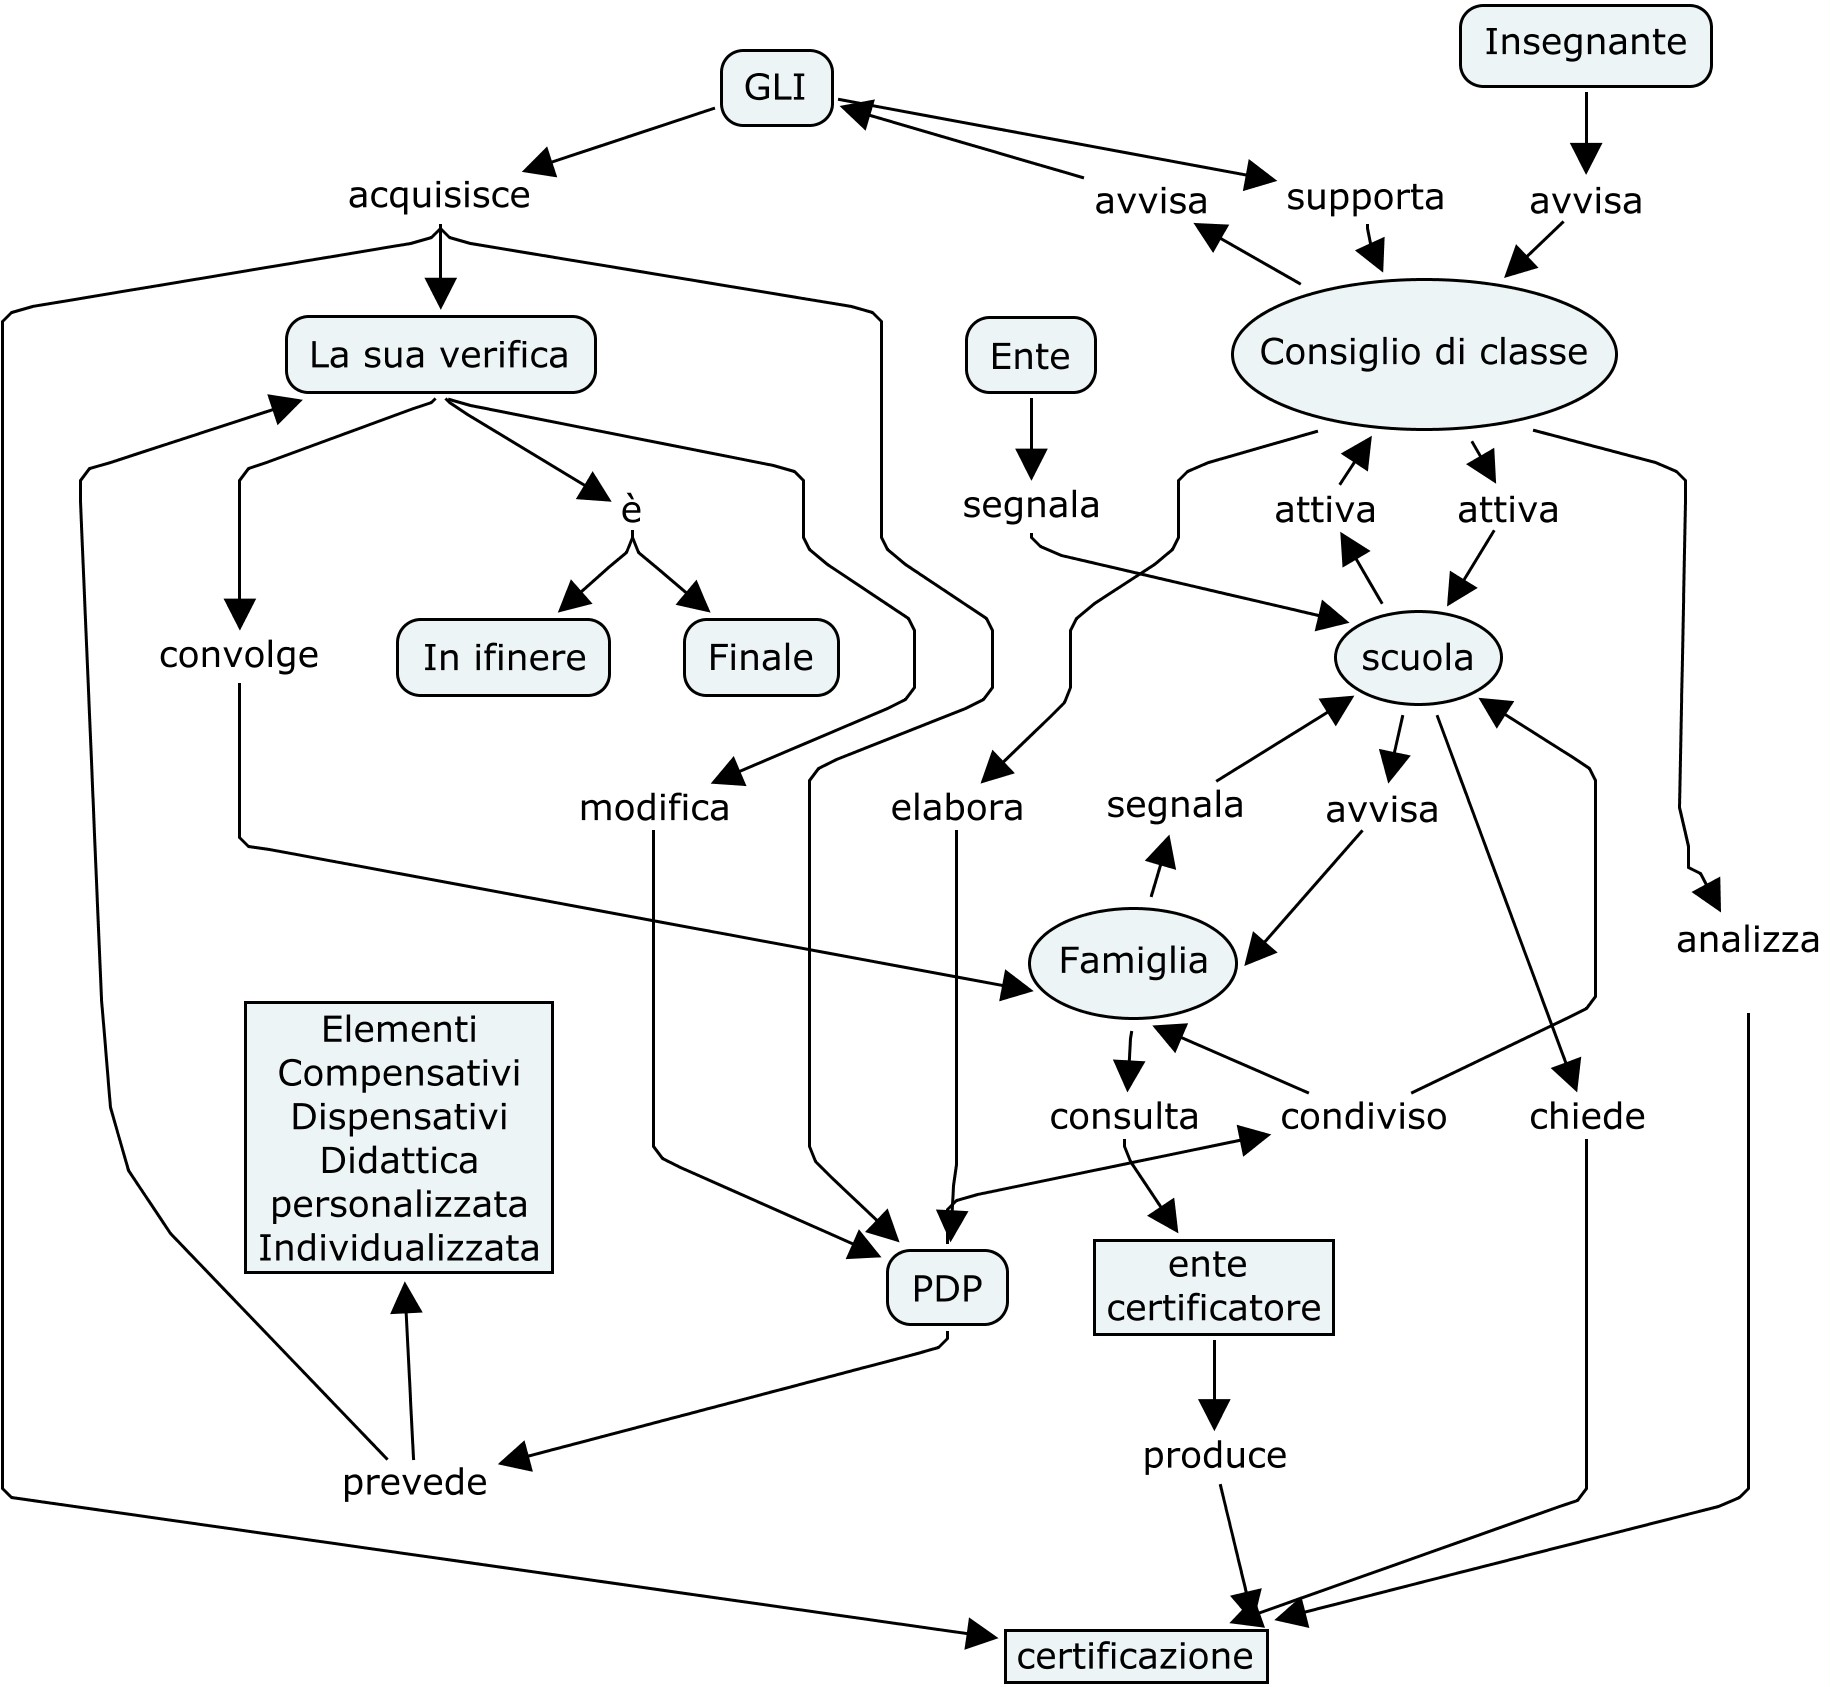
\includegraphics[scale=0.23]{bes3.jpg}
%\end{center}
Possiamo classificar i BES in tre gruppi, Lo schema\vref{fig:besschema} mostra a grandi linee cosa prevede la normativa. 
 \begin{figure}[t]
 	\centering
 	\includegraphics[width=1\linewidth, height=1\textheight]{bes schemab.pdf}
 	\caption[Classificazione]{Classificazione}
 	\label{fig:besschema}
 \end{figure}
La gestione degli alunni in BES è molto complessa. La procedura\vref{fig:bes3} che segue mostra come tre entità: la famiglia, la scuola, il Consiglio di Classe possono interagire per prendere in carica lo studente. Nella schema è presente anche il GLI, che ha funzioni di coordinamento, supporto e raccolta di informazioni. Lo schema dovrebbe essere condiviso con tutti in modo che ogni componente del sistema sa cosa deve fare. 
\begin{figure}[t]
\centering
\includegraphics[width=1\linewidth, height=1\textheight]{bes3c}
\caption[Gestione BES]{Proposta di gestione di un alunno con BES}
\label{fig:bes3}
\end{figure}




\chapter{Quadro Sinottico BES}\footcite{Nocera2014a}
\label{char:QuadroSinotticoBES}
\begin{longtable}{p{0.2\textwidth}p{0.4\textwidth}p{0.2\textwidth}p{0.2\textwidth}}
\toprule
 &\textbf{Disabilità}&\textbf{DSA}&\textbf{BES}  \\
\midrule
\endfirsthead
\toprule
 &\textbf{Disabilità}&\textbf{DSA}&\textbf{BES}  \\
\midrule
\endhead
\textbf{Individuazione degli alunni}&Certificazione ai sensi legge 104/92\footcite{Legge_104_92} Art 3 commi 1 e 3 &Diagnosi ai senso legge 170/10\footcite{legge170}&Delibera del consiglio di classe ai sensi della direttiva ministeriale 271/12/2012\footcite{dir27Dic2012} e CM 8/13\footcite{cm8_2013} e Nota 22/11/2013\footcite{Nota_2563_2013}\\
\midrule
\textbf{Strumenti didattici}&\textbf{PEI:} con riduzione di talune discipline (art 16 Legge 194/92)\footcite{Legge_104_92} e prove equipollenti e tempi più lunghi (art. 16 comma 3 legge 104/92)\footcite{Legge_104_92}

 Insegnate per il sostegno e/o assistenti per l'autonomia e la comunicazione.&\textbf{PDP:} con strumenti compensativi e/o misure dispensative e tempi più lunghi. &\textbf{PDP:} (solo se prescrive strumenti compensativi e/o misure dispensative) \\
 \midrule
 \textbf{Effetti sulla valutazione del profitto}&
\textbf{PRIMO CICLO:}
 
 \textbf{1) Valutazione positiva} 
 
 (art. 16 commi 1 e 2 L. n 104/92): se si riscontrano miglioramenti rispetto ai livelli iniziali degli apprendimenti relativi ad un PEI formulato solo con riguardo alle effettive capacità dell'alunno.
 
 \textbf{2) Attestato con i crediti formativi:}
 
 eccezionalmente in caso di mancati o insufficienti progressi rispetto ai livelli iniziali degli apprendimenti. Rilasciato dalla Commissione d'esame e non dalla scuola. È comunque titolo idoneo all'iscrizione al secondo ciclo (O.M. n 90/01, art. 11 comma 12\footcite{OM_90_2001})
 
\textbf{SECONDO CICLO:}

\textbf{ 1) Programmazione semplificata:} diritto al diploma, se superato positivamente esame di Stato con prove equipollenti e tempi più lunghi

 \textbf{2) Programmazione differenziata:} diritto ad attestato certificante i crediti formativi (rilasciato sempre dalla commissione d'esame e non dalla scuola) 
 &
 \textbf{1) Dispensa scritto lingue straniere compensata da prova orale:} consente Diploma (Linee guida\footcite{LineGuida2011} 4.4 allegate a D.M. 12/07/2011, art. 6 comma 5\footcite{DM_122_2011}).
 
 \textbf{2) Esonero lingue straniere:} solo attestato con i crediti formativi (D.M. 12/07/2011 art. 6 comma 6).
 &Misure dispensative (ad eccezione della dispensa dallo scritto di lingue straniere e dell'esonero normativamente previste solo per DSA).
 
 Strumenti compensativi.
 
 Tempi più lunghi,
 
 Con possibile Diploma.
 
 Per gli stranieri c'è normativa specifica\footcite{CM_2_2010}\footcite{MIUR2007}\footcite{CM_24_2006}.\\
 \bottomrule
\end{longtable}
\chapter{Esempi di regolamento per i GLI}
\section*{Regolamento del GLI (Gruppo di lavoro per l'inclusione) d'Istituto}
\begin{description}
	\item[Art.1] -- Composizione 
	
	Presso il nostro Istituto\footcite{IISGGasparriniMelfi2013} viene costituito, conformemente all'art. 15 comma 2 della legge quadro
	5/02/1992 n.104 e alla restante normativa di riferimento, il Gruppo di Lavoro per l'inclusione, il cui
	compito, oltre a quello di collaborare all'interno dell'istituto alle iniziative educative e di
	integrazione che riguardano studenti con disabilità o con disturbi specifici di apprendimento (DSA),
	si estende alle problematiche relative a tutti i BES.
	
	Il GLI d'Istituto è composto da:
	\begin{enumerate}
		\item  il Dirigente scolastico, che lo presiede;
		\item  il Docente referente del GLH e dei DSA;
		\item  i coordinatori dei Consigli di classe in cui siano presenti alunni con disabilità (e con DSA);
		\item un docente curricolare;
		\item  i docenti specializzati per le attività di sostegno degli alunni con disabilità certificata;
		\item un rappresentante dei genitori di studenti con disabilità (e/o DSA)
		\item un rappresentante degli studenti con disabilità (e/o DSA)
		\item  un rappresentante degli studenti
		\item uno o più rappresentanti degli operatori sociali o sanitari che al di fuori dell'Istituto si occupano
		degli alunni BES.
	\end{enumerate}
	\item [Art.2] -- Convocazione e Riunioni
	
	Le riunioni sono convocate dal Dirigente Scolastico e presiedute dallo stesso o da un suo delegato.
	Le deliberazioni sono assunte a maggioranza dei componenti.
	Di ogni seduta deve essere redatto apposito verbale.
	Il GLI si può riunire in seduta plenaria (con la partecipazione di tutti i componenti), ristretta (con
	la sola presenza degli insegnanti), o dedicata (con la partecipazione delle persone che si occupano
	in particolare di un alunno). In quest'ultimo caso il GLI è detto operativo.
	Gli incontri di verifica con gli operatori sanitari sono equiparati a riunioni del GLI in seduta
	dedicata.
	\item [Art.3] -- Competenze
	
	Il GLI d'Istituto presiede alla programmazione generale dell'integrazione scolastica nella scuola ed
	ha il compito di collaborare alle iniziative educative e di integrazione previste dal piano educativo
	individualizzato dei singoli alunni attraverso l'attuazione di precoci interventi atti a prevenire il
	disadattamento e l'emarginazione e finalizzati alla piena realizzazione del diritto allo studio degli
	alunni con disabilità.
	
	In particolare il GLI svolge le seguenti funzioni:
	\begin{enumerate}
		\item rilevare i BES presenti nella scuola;
		\item elaborare una proposta di Piano Annuale per l'Inclusività riferito a tutti gli alunni con BES,
		da redigere al termine di ogni anno scolastico (entro il mese di giugno, discusso e deliberato
		in Collegio dei Docenti e inviato ai competenti Uffici degli UUSSRR, nonché ai GLIP e al
		GLIR);
		\item rilevare, monitorare e valutare il livello di inclusività della scuola;
		\item gestire e coordinare l'attività dell'Istituto in relazione agli alunni con disabilità al fine di
		ottimizzare le relative procedure e l'organizzazione scolastica;
		\item  analizzare la situazione complessiva dell'istituto (numero di alunni con disabilità, DSA,
		BSE, tipologia dello svantaggio, classi coinvolte);
		\item individuare i criteri per l'assegnazione degli alunni con disabilità alle classi;
		\item individuare i criteri per l'assegnazione dei docenti di sostegno alle classi, per la
		distribuzione delle ore delle relative aree e per l'utilizzo delle compresenze tra i docenti;
		\item definire le linee guida per le attività didattiche di sostegno agli alunni con disabilità
		dell'Istituto da inserire nel POF;
		\item seguire l'attività dei Consigli di classe e degli insegnanti specializzati per le attività di
		sostegno, verificando che siano attuate le procedure corrette e che sia sempre perseguito il
		massimo vantaggio per lo sviluppo formativo degli alunni nel rispetto della normativa;
		\item proporre l’acquisto di attrezzature, strumenti, sussidi, ausili tecnologici e materiali didattici
		destinati agli alunni con disabilità e DSA o ai docenti che se ne occupano;
		\item definire le modalità di accoglienza degli alunni con disabilità;
		\item analizzare casi critici e proposte di intervento per risolvere problematiche emerse nelle
		attività di integrazione;
		\item formulare proposte per la formazione e l'aggiornamento dei docenti.
	\end{enumerate}
	\item [Art.4] -- Competenze del referente del GLH
	
	Il Docente Referente del GLH si occupa di:
	\begin{enumerate}
		\item  convocare e presiedere, su delega del Dirigente Scolastico, le riunioni del GLH;
		\item predisporre gli atti necessari per le sedute del GLH;
		\item verbalizzare le sedute del GLH;
		\item curare la documentazione relativa agli alunni con disabilità, verificarne la regolarità e aggiornare
		i dati informativi (generalità, patologie, necessità assistenziali e pedagogiche, ecc.), sostenendone la
		sicurezza ai sensi del Documento programmatico sulla sicurezza dei dati personali e sensibili
		dell'Istituto;
		\item collaborare col Dirigente Scolastico all'elaborazione dell'orario degli insegnanti di sostegno,
		sulla base dei progetti formativi degli alunni e delle contingenti necessità didattico-organizzative;
		\item collaborare col Dirigente Scolastico alla elaborazione del quadro riassuntivo generale della
		richiesta di organico dei docenti di sostegno sulla base delle necessità formative degli alunni con
		disabilità desunte dai relativi PEI e dalle relazioni finali sulle attività di integrazione messe in atto
		dai rispettivi Consigli di classe;
		\item collaborare all'accoglienza dei docenti specializzati per le attività di sostegno;
		\item curare l'espletamento da parte dei Consigli di classe o dei singoli docenti di tutti gli atti dovuti
		secondo le norme vigenti;
		\item tenere i contatti con gli EE.LL. e con l'Unità multidisciplinare;
		\item curare l'informazione sulla normativa scolastica relativa all'integrazione degli alunni disabili;
		\item  curare, in collaborazione con l'Ufficio di Segreteria, le comunicazioni dovute alle famiglie e/o
		all'Ufficio Scolastico Territoriale di competenza.
	\end{enumerate}
	\item [Art.5] -- Competenze della Commissione per gli alunni con disabilità
	
	All'interno del Gruppo di lavoro sull'handicap i docenti di sostegno della scuola costituiscono una
	Commissione che si occupa degli aspetti che più strettamente riguardano le attività didattiche dei
	Consigli di Classe in cui sono presenti alunni con disabilità, ed in particolare di:
	\begin{enumerate}
		\item  analisi e revisione del materiale strutturato utile ai docenti per migliorare gli aspetti della
		programmazione (modello PDF, modello di PEI, relazione iniziale e finale, ecc..);
		\item sostegno, informazione e consulenza per i docenti riguardo le problematiche relative
		all'integrazione scolastica degli alunni con disabilità;
		\item individuazione di strategie didattiche rispondenti ai bisogni delle specifiche disabilità;
		\item collaborazione con gli specialisti che seguono periodicamente i ragazzi con disabilità;
		\item analisi dell'andamento didattico-disciplinare degli alunni con disabilità;
		\item segnalazione di casi critici e di esigenze di intervento rese necessarie da difficoltà emerse nelle
		attività di integrazione;
		\item sostegno alle famiglie;
		\item analisi degli elementi utili alla definizione della proposta per l’organico dei docenti di sostegno.
	\end{enumerate}
	\item [Art. 6] --  Competenze dei docenti specializzati per le attività di sostegno
	
	I docenti specializzati per le attività di sostegno devono inoltre:
	\begin{enumerate}
		\item informare gli altri membri del Consiglio di Classe sulle problematiche relative all'alunno
		con disabilità e sulle procedure previste dalla normativa;
		\item redigere il PDF e il PEI in versione definitiva;
		\item seguire l'attività educativa e didattica degli alunni con disabilità a loro affidati, secondo le
		indicazioni presenti nei relativi PEI;
		\item mediare, in collaborazione con il Coordinatore di classe, le relazioni tra il Consiglio di
		Classe e la famiglia dell'alunno con disabilità;
		\item relazionare sull'attività didattica svolta per gli alunni con disabilità e su qualsiasi problema
		che emerga rispetto all'integrazione scolastica.
	\end{enumerate}
	\item [Art. 7] -- Competenze dei Consigli di classe con alunni con disabilità
	
	I Consigli di Classe in cui siano inseriti alunni con disabilità, devono:
	\begin{enumerate}
		\item essere informati sulle problematiche relative all'alunno con disabilità per quanto è
		necessario all'espletamento dell'attività didattica;
		\item essere informati sulle procedure previste dalla normativa;
		\item discutere e approvare il percorso formativo più opportuno per l'alunno;
		\item definire e compilare la documentazione prevista (PDF; PEI) entro le date stabilite;
		\item  effettuare la verifica del PEI nei tempi e nelle modalità previsti, allo scopo di prevedere
		eventuali modificazioni e miglioramenti adeguati alle difficoltà riscontrate e valorizzare le
		pratiche di successo.
	\end{enumerate}
	\item [Art. 8] -- Competenze dei singoli docenti curricolari
	
	I singoli docenti che seguono alunni con disabilità, oltre a quanto descritto nell'art. 7, devono:
	\begin{enumerate}
		\item contribuire, in collaborazione con l'insegnante specializzato, all'elaborazione del P.E.I;
		\item seguire per gli alunni con disabilità le indicazioni presenti nei PEI relativi riguardo agli
		obiettivi, alle metodologie e attività e alle modalità di verifica e valutazione;
		\item segnalare al Coordinatore di classe, all'insegnante specializzato e al Referente del GLH
		qualsiasi problema inerente l'attività formativa che coinvolga gli alunni con disabilità;
		\item il docente coordinatore di Classe parteciperà agli incontri di verifica con gli operatori
		sanitari.
	\end{enumerate}
\end{description}

I singoli docenti oltre a quanto stabilito negli articoli precedenti, devono segnalare al Coordinatore
di classe, all'insegnante di sostegno o al Referente del GLH qualsiasi problema inerente l'attività
formativa che coinvolga alunni con disabilità certificate o disturbi specifici di apprendimento.
\section*{Regolamento del  Gruppo di Lavoro per l'Inclusione (GLI)}
Il Gruppo di Lavoro per l'Inclusione\footcite{ISISLinoZanussiPordenone2013} è istituito in conformità all'art.15 comma 2 della
L.104/92 per attuare un'efficace capacità di rilevazione e intervento relativi alle
problematiche degli allievi con bisogni educativi speciali (BES) in relazione alla Circolare
MIUR N. 8 del 6 Marzo 2013, prot. N. 561 \cit{strumenti d'intervento per alunni con Bisogni
Educativi Speciali}.
Il GLI dura in carica un anno e si riunisce in seduta plenaria o ristretta normalmente ogni
due mesi.
Il GLI è costituito da:
\begin{itemize}
	\item Dirigente Scolastico, che lo presiede
	\item Docente referente del GLI
	\item  Docenti di sostegno
	\item Docente referente DSA
	\item  Docenti curricolari
	\item Docente referente per l'intercultura
\end{itemize}
Possono partecipare alle riunioni assistenti alla comunicazione, coordinatori di classe,
genitori ed esperti istituzionali o esterni in regime di convenzionamento con la scuola.
\subsection*{COMPITI DEL GLI}
Il GLI ha il compito di:
\begin{itemize}
	\item Rilevare i BES presenti nella scuola
	\item  Raccogliere e documentare gli interventi didattico-educativi posti in essere o da
	progettare per gli allievi con bisogni educativi speciali
	\item Confrontarsi sui casi, dare consulenza e supporto ai colleghi sulle strategie e
	metodologie nella gestione dei BES all'interno di ogni classe
	\item Rilevare e monitorare il livello di inclusività dei BES all'interno dell'Istituto
	\item Accogliere eventuali proposte di lavoro del GLH operativo nella scuola
	\item Elaborare le proposte per il Piano Annuale per l'Inclusività riferito a tutti gli alunni
	con BES da redigere al termine di ogni anno scolastico (entro il mese di giugno)
\end{itemize}
Approvato dal Consiglio d'Istituto in data 12/04/2013
\chapter{Bisogni Educativi Speciali. Approfondimenti sulla redazione del piano annuale per l'inclusività }

Oggetto: \textbf{ Bisogni Educativi Speciali. Approfondimenti in ordine alla redazione del piano
annuale per l'inclusività nell'ottica della personalizzazione dell'apprendimento.\footcite{USRperLEmiliaRomagna2013a}}

Materiali per la formazione dei docenti a.s. 2013-2014.

Nell'imminenza dell'avvio del prossimo anno scolastico 2013-2014 si richiama l'attenzione dei docenti
e dei Dirigenti Scolastici dell'Emilia-Romagna su alcuni punti essenziali del ricco dibattito culturale sul
tema dei bisogni educativi speciali, apertosi con la Direttiva 27 dicembre 2012, la Circolare Ministeriale
8/2013 e la nota del Capo Dipartimento Istruzione prot.1551 del 27 giugno 2013.
Nell'invitare ad una lettura coordinata dei diversi documenti, si ritiene utile riprenderne alcuni assunti,
anche in relazione a quanto già indicato da questo Ufficio con la nota prot.6721 del 29 maggio 2013
(reperibile nel settore BES del sito Internet di questa Direzione Generale unitamente ai documenti
ministeriali citati).
A questo Ufficio sono infatti pervenute sollecitazioni ad approfondire il tema della personalizzazione
dei percorsi di insegnamento/apprendimento e delle modalità di trascrizione di tali percorsi nel piano
annuale per l'inclusività , per fornire una base comune di indirizzo alle scuole della regione.
La nota ministeriale prot.1551/2013 sottolinea che il Piano annuale per l'inclusività non va
\cit{interpretato come un piano formativo per gli alunni con bisogni educativi speciali} ma come uno
\cit{strumento di progettazione} dell'offerta formativa delle scuole \cit{in senso inclusivo, è lo sfondo ed il
fondamento sul quale sviluppare una didattica attenta ai bisogni di ciascuno nel realizzare gli obiettivi
comuni}.
Viene inoltre confermato che la redazione del PAI non deve fornire l'occasione per categorizzare le
persone ma per individuare le situazioni problematiche e le strategie per farvi fronte, qualificando le
modalità di insegnamento.
In via preliminare va richiamata l'attenzione al linguaggio usato. In pochissimo tempo sta già entrando
nell'uso comune l'espressione “ragazzi BES”, non accettabile e non rispettosa. Coloro che lavorano
nella comunicazione educativa hanno il dovere di usare un linguaggio attento alle persone. Non è
questione di formalismo nominale, è questione sostanziale: \cit{Non esiste una cosa come il lettore
innocente. Le parole sono ricevute e collocate nel contesto interpretativo che noi costruiamo leggendo
la pagina. Questo processo è definito sia dal nostro background culturale, sia dalle esperienze sia dai nostri oggettivi limiti. Di conseguenza è necessario pensare attentamente al linguaggio che usiamo}
(Roger Slee, Inclusion in practice, Educational Review 2001 ).
Il rischio di catalogare persone anziché individuare problemi ed elaborare strategie di soluzione, non
riguarda soltanto il nostro Paese. Nel dibattito internazionale, infatti, da alcuni decenni si vanno
affrontando temi e prospettive di grande rilievo culturale e professionale, che conviene richiamare
all'attenzione del personale scolastico ed educativo.
I punti approfonditi nella presente nota sono i seguenti:
\begin{description}
	\item[A]] SPUNTI DAL DIBATTITO INTERNAZIONALE
	\begin{description}
		\item[1)] Bisogni speciali o diritti specifici?
		\item [2)] l'educazione inclusiva
		\item [3)] l'insegnante inclusivo
		\item [4)] Universal Design for Learning (UDL)
	\end{description} 
	\item [B]] IL PIANO ANNUALE PER L'INCLUSIVITA' (PAI)
	\begin{description}
		\item[5)] Scopi del PAI
		\item [6)] Punti essenziali da trattare tra POF e PAI
		\item [7)] Il PAI e le risorse professionali della scuola (o delle scuole in rete)
		\item [8)] il PAI e la razionalizzazione dell'uso delle risorse (anche economiche)
	\end{description}
	\item [C]] I PIANI PERSONALIZZATI E L'ADATTAMENTO DEI CURRICOLI
	\item [D]] AFFRONTARE LE SITUAZIONI DIFFICILI
	\begin{description}
		\item[9)] Evitare la riduzione in schede
		\item [10)] Esaminare i problemi
		\begin{description}
			\item[l0.1] il problema dei comportamenti-problema
			\item[l0.2] il problema dei comportamenti auto ed etero aggressivi
		  \item[l0.3] Il problema dei problemi \cit{invisibili}
		  \item[l0.4] il problema delle difficoltà di apprendimento
		\end{description}
		\item[l1)] Curare la formazione
	\end{description}
\end{description}
\begin{description}
	\item[A]] SPUNTI DAL DIBATTITO INTERNAZIONALE
	\begin{enumerate}
		\item Bisogni speciali o diritti specifici?
		
		Nel 2000, l'UNESCO, con il {\foreignlanguage{english} Dakar Framework for Action} ha definito il principio dell'Educazione per tutti {\foreignlanguage{english}	(Education For All - EFA)}
	 ponendolo come obiettivo dell'azione dei Governi, da raggiungere entro il
		2015. Anche se l'obiettivo è ben lontano dall'essere centrato, il fatto che sia stato posto costituisce un
		elemento culturale imprescindibile nel quadro educativo attuale.
		
		Il {\foreignlanguage{english} Dakar Framework for Action} ed i documenti UNESCO ad esso collegati, trattano il tema
		dell'acquisizione, da parte di ciascuna persona, degli elementi fondamentali dell'educazione. \cit{Ogni
		persona –- bambino, ragazzo e adulto -- deve poter fruire di opportunità educative specificamente
		strutturate per incontrare i propri basilari bisogni di educazione. Questi bisogni comprendono tanto i
		contenuti essenziali dell'apprendimento (dal linguaggio orale e scritto, alla matematica alla capacità 
		di risolvere i problemi) quanto gli strumenti della conoscenza, le competenze, i valori e lo sviluppo delle
		attitudini, cioè quanto richiesto ad un essere umano per sopravvivere, sviluppare in pieno le proprie
		capacità , vivere e lavorare dignitosamente, partecipare allo sviluppo, migliorare la qualità della propria
		vita, prendere decisioni informate, continuare ad apprendere} ({\foreignlanguage{english} Dakar Framework for Action}, Art.1).
	
		Nell'ottica delineata dal documento di Dakar (e da altri documenti internazionali) il termine inglese
			\cit{needs} corrisponde quindi più al concetto di \cit{diritti} che a quello di \cit{bisogni}. I \cit{{\foreignlanguage{english}basic educational needs}} del documento di Dakar potrebbero essere concettualmente tradotti con l'espressione italiana \cit{diritti educativi essenziali}. La riflessione dei delegati UNESCO ricorda che tali diritti non sono fissi
		ma variano in relazione ai contesti, alla storia, alla cultura, alle condizioni, al divenire dell'esperienza
		umana.
	
		\'{E} quindi compito delle comunità educanti individuare per ogni persona, in ciascuno specifico
		momento della vita e nelle condizioni in cui oggettivamente essa si trova, quali siano i diritti educativi
		essenziali, elaborando le più efficaci strategie per raggiungerli.
		
		Ecco quindi che si profila la possibilità di una ulteriore possibile sfumatura del lessico: tradurre \cit{{\foreignlanguage{english}Education For All}}
		 con l'espressione \cit{educazione per tutti} può indurre in errore. La scuola
		dell'obbligo, ad esempio, potrebbe già di per sé rispondere alla richiesta.
	
		Ma, nei propri documenti, l'UNESCO ammonisce in merito al fatto che l'espansione delle opportunità 
		educative non si traduce automaticamente in uno sviluppo significativo delle persone e della società .
		Occorre che l'educazione fornisca risultati efficaci e non soltanto che consenta ad un maggior numero
		di persone di frequentare contesti scolastici 
		\begin{otherlanguage}{english}
	(“ Whether or not expanded educational opportunities will
	translate into meaningful development - for an individual or for society - depends ultimately on whether
	people actually learn as a result of those opportunities, i.e., whether they incorporate useful knowledge,
	reasoning ability, skills, and values. The focus of basic education must, therefore, be on actual learning
	acquisition and outcome, rather than exclusively upon enrolment, continued participation in organized
	programmes and completion of certification requirements. Active and participatory approaches are
	particularly valuable in assuring learning acquisition and allowing learners to reach their fullest potential.
	It is, therefore, necessary to define acceptable levels of learning acquisition for educational programmes
	and to improve and apply systems of assessing learning achievement” . The Dakar Framework for
	Action, Art.4). 
		\end{otherlanguage}
		
		Pertanto l'UNESCO richiama il dovere degli Stati non soltanto di dichiarare l'assolvimento dei diritti
		educativi essenziali ma anche di assolverli effettivamente ed in modo efficace, fornendo risultati
		documentati attraverso idonee modalità di valutazione (assessment).
		Quindi la traduzione pedagogica della definizione dell'UNESCO potrebbe essere quella dell'educazione
		per ciascuno.
		
		Questo è l'aggancio, nella nostra legislazione, con il principio della personalizzazione introdotto con la
		Legge 53/2003, preceduta fin dal 1977 dalla Legge 517 che definì sia l'inclusione dei ragazzi con
		disabilità nella scuola comune sia il principio dell'individualizzazione dell'insegnamento con nuovi
		criteri di valutazione.
		
		Può essere interessante riflettere sul fatto che anche nel Regno Unito di Gran Bretagna sussistono
		concezioni diverse degli \cit{{\foreignlanguage{english}Special Educational Needs (SEN)}}; ad esempio, le disposizioni scozzesi 
		({\foreignlanguage{english}Scottish
		Executive} 2004, aggiornate nel 2009) denominate \cit{{\foreignlanguage{english}The Additional Support for Learning Act}}
		sostituiscono la dizione \cit{bisogni educativi speciali} con quella più ampia di \cit{supporti aggiuntivi
		all'apprendimento e di modalità diverse di insegnamento} 
	(\cit{\begin{otherlanguage}{english}
		provision wich is additional to, or
		otherwise different from, the educational provision made generally for children or … young persons of
		the same age in schools
	\end{otherlanguage}}).
		
		La norma scozzese ricorda che ogni ragazzo, in qualsiasi punto della sua carriera scolastica, per
		un'ampia varietà di ragioni, può avere bisogno di supporti aggiuntivi all'insegnamento (o di
		diversificazione dell'insegnamento) ed ha diritto a riceverli.
		Tuttavia anche questa accezione non corrisponde in pieno alla logica inclusiva, in quanto comunque
		identifica un range ritenuto comune, discostandosi dal quale si ha diritto a interventi specificamente
		mirati e intensificati (quindi fa riferimento ad un concetto di normalità definito dalla media delle
		risposte e di bisogno aggiuntivo come risposta ad un discostamento significativo da tale media).
		\item L'educazione inclusiva
		
		Il programma di Dakar è corredato da una serie di note che approfondiscono e specificano i temi
		succintamente definiti nei punti del programma stesso, riportando i contenuti della discussione
		preliminare. In tali note viene ricordato che l'{\foreignlanguage{english}Education For All} è un concetto inclusivo e che è pertanto urgente \cit{includere coloro che sono socialmente, culturalmente ed economicamente esclusi. Ciò
		richiede lo sviluppo … di approcci all'apprendimento diversi, flessibili e innovativi e di contesti che
		inducano al rispetto reciproco e alla fiducia} (punto 65).
		
		L'importanza che l'UNESCO assegna all'educazione inclusiva è ribadita in molti documenti, ad esempio
		nelle \begin{otherlanguage}{english}
		Conclusions ad Recommendations of the 48th Session of the International Conference on
		Education
		\end{otherlanguage}
		 Ginevra 2008: \cit{L'educazione inclusiva è un processo continuo che mira ad offrire educazione
		di qualità per tutti rispettando diversità e differenti bisogni e abilità , caratteristiche e aspettative
		educative degli studenti e delle comunità , eliminando ogni forma di discriminazione}.
		
		L'intenso dibattito internazionale sulla scuola inclusiva sta facendo emergere riflessioni per nulla
		scontate. Una delle più rilevanti è la differenza che esiste tra la concezione definita \cit{{\foreignlanguage{english}mainstreaming}}
		e quella \cit{inclusiva}. Con il termine \cit{{\foreignlanguage{english} mainstream}} nel mondo anglosassone si indicano le scuole che,
		adottando un curricolo specifico, accettano gli allievi con disabilità o in difficoltà soltanto se sono in
		grado di seguire il curricolo con una minima assistenza.
		
		Gli {\foreignlanguage{english}Special Educational Needs} (nelle varie accezioni) ampliano l'accoglienza scolastica mantenendo
		tuttavia la distinzione tra percorsi comuni (e quindi normali) e percorsi differenziati (e quindi speciali).
		I sostenitori dell'educazione inclusiva (in tutto il mondo) ritengono che queste non siano le risposte
		corrette perché soltanto nelle scuole inclusive gli insegnanti sono tenuti a modificare i loro stili di
		insegnamento per incontrare lo stile di apprendimento di ciascun allievo.\begin{otherlanguage}{english}
		\cit{School of the future need to
		ensure theat each student receives the individual attention, accomodations and supports theat will
		result in meaningful learning} (NVPE Nevada Partnership for inclusive education).
		\end{otherlanguage} 
		
		Le istituzioni scolastiche dell'Emilia-Romagna sono quindi invitate a riflettere sul fatto che la semplice
		presenza degli alunni disabili o con DSA o in difficoltà non basta a costruire una scuola inclusiva. Non
		bastano neppure i piani educativi individualizzati o personalizzati. Occorre che il modo di insegnare e
		di valutare cambi, per poter essere \cit{curvato} sulle diverse situazioni ed in relazione a diverse difficoltà .
		
		Ecco perché la nota ministeriale prot.1551/2013 definisce il PAI non come un \cit{documento} ma come
		uno \cit{strumento} che deve contribuire ad \cit{accrescere la consapevolezza dell'intera comunità educante
		sulla centralità e la trasversalità dei processi inclusivi in relazione alla qualità dei risultati educativi}.
		Senza questo passaggio qualitativo, qualunque riflessione resterebbe sterile.
		
		Quindi, come già ricordato nella precedente nota di questo Ufficio prot.6721/2013, i primi passi da
		effettuare sono quelli relativi all'effettiva inclusività della scuola e sulle capacità inclusive dei docenti.
		Non si tratta di ripetere le rituali parole dell'inclusione; si tratta di esplorare nel merito il modo di
		organizzare la scuola e di insegnare, scuola per scuola, docente per docente, alunno per alunno.
		
		Per approfondire i percorsi di auto-riflessione delle scuole sulla propria azione in termini di inclusione,
		si ricordano due importanti strumenti di lavoro, entrambi disponibili gratuitamente sul web.
		
		Il primo strumento è di derivazione inglese ma è disponibile in lingua italiana; si tratta dell'Index per
		l'inclusione di Toni Booth e Mel Ainscow.
	
		Il secondo strumento è il software Quadis elaborato dall'Ufficio Scolastico Regionale per la Lombardia.
		Per entrambi i link sono disponibili nel settore “Bisogni educativi speciali” del sito Internet di questa
		Direzione Generale \url{www.istruzioneer.it} cui si rimanda anche per materiali di approfondimento e di
		documentazione su vari argomenti.
		\item L'insegnante inclusivo
		
		Può essere interessante riprendere un documento elaborato dalla {\foreignlanguage{english}European Agency for Development} in {\foreignlanguage{english}Special Needs Education} \cit{Profilo dei docenti inclusivi} 2012, in cui tale profilo viene puntualizzato
		in quattro valori, ciascuno dei quali declinato in un interessante elenco di indicatori, sui quali le scuole
		potrebbero aprire una attenta riflessione, proprio in relazione alla stesura del PAI.
		
		I quattro valori di riferimento condivisi dai docenti inclusivi sono:
		\begin{description}
			\item[I] (Saper) valutare la diversità degli alunni – la differenza tra gli alunni è una risorsa e una
			ricchezza
			\item [II] Sostenere gli alunni – i docenti devono coltivare aspettative alte sul successo scolastico degli
			studenti
			\item [III] Lavorare con gli altri – la collaborazione e il lavoro di gruppo sono approcci essenziali per tutti
			i docenti
			\item [IV] Aggiornamento professionale continuo – l'insegnamento è una attività di apprendimento e i
			docenti hanno la responsabilità del proprio apprendimento permanente per tutto l'arco della
			vita.
		\end{description}
		 
		L'elenco degli indicatori proposti nella pubblicazione citata è molto lungo e dettagliato. Se ne
		segnalano qui soltanto alcuni tra quelli ritenuti più significativi:
		\begin{itemize}
			\item l'integrazione scolastica è una riforma sociale non negoziabile;
			\item l'accesso all'istruzione dell'obbligo in classi comuni non basta;
			\item partecipazione significa che gli alunni devono essere impegnati in attività di apprendimento
			utili ed importanti per loro;
			\item l'inclusione si delinea in termini di presenza (accesso all'istruzione), partecipazione (qualità 
			dell'esperienza di apprendimento) e conseguimento (dei risultati educativi e del successo
			scolastico) di tutti gli studenti;
			\item la classificazione e la catalogazione degli alunni può avere un impatto negativo sulle
			opportunità di apprendimento;
			\item i docenti devono capire i percorsi tipici e atipici della crescita;
			\item gli insegnanti capaci insegnano a tutti gli alunni;
			\item i metodi di valutazione devono incentrarsi sui punti di forza di un allievo.
		\end{itemize}
		
		Per una lettura più approfondita si rimanda alla pubblicazione citata, richiamando la necessità che
		ciascun docente e ciascun collegio si soffermino a riflettere sul profilo ivi tratteggiato. Anche il link di
		questo documento è reperibile nel sito Internet di questo Ufficio indicato al precedente punto.
		
		Tra le ricerche più interessanti a livello internazionale in merito alla personalizzazione
		dell'insegnamento (e quindi sostenere l'attuazione di una reale inclusività ), si ritiene particolarmente
		utile quella denominata \cit{{\foreignlanguage{english}Universal Design for Learning}}.
		\item Universal Design for Learning (UDL)
		
		L'espressione {\foreignlanguage{english}Universal Design for Learning (UDL)} indica una modalità di progettazione e di gestione
		della pratica educativa volta ad incontrare le diverse modalità di apprendimento e le diverse condizioni
		che possono presentarsi nei diversi contesti (principalmente scolastici).
		I suggerimenti concreti, i materiali e gli strumenti informatici messi a disposizione su Internet, i molti
		esempi concreti possono risultare di grande utilità anche agli insegnanti italiani, per cui si rimanda alla
		scheda di approfondimento allegata alla presente nota (Allegato 1).
		
	\end{enumerate}
	\item [B] IL PIANO ANNUALE PER L’INCLUSIVIT\'{A} (PAI)
	\begin{enumerate}
		\setcounter{enumi}{4}
		\item Scopi del PAI
		
		Appurato dunque che il PAI non è un documento burocratico ma uno strumento di auto riflessione
		delle scuole nell'ottica del raggiungimento del successo formativo degli allievi e del benessere
		psicologico nei contesti scolastici, si può cercare di suggerire alcune, più dettagliate, piste di lavoro.
		
		Il piano annuale per l'inclusività è il coronamento del lavoro svolto in ciascun anno scolastico e
		costituisce il fondamento per l'avvio del lavoro dell'anno scolastico successivo.
		
		La redazione del PAI e l'assunzione collegiale di responsabilità in relazione alla sua stesura,
		realizzazione e valutazione ha lo scopo di:
		\begin{description}
			\item[--] garantire l'unitarietà dell'approccio educativo e didattico dell'istituzione scolastica
			\item[--] garantire la continuità dell'azione educativa e didattica anche in caso di variazione dei docenti
			e del dirigente scolastico (continuità orizzontale e verticale)
			\item[--] consentire una riflessione collegiale sulle modalità educative e sui metodi di insegnamento
			adottati nella scuola, arrivando a scelte basate sull'efficacia dei risultati in termini di
			comportamento e di apprendimento di tutti gli alunni
			\item[--] individuare le modalità di personalizzazione risultate più efficaci in modo da assicurarne la
			diffusione tra gli insegnanti della scuola e tra scuole diverse
			\item[--] raccogliere i piani educativi individualizzati ed i piani didattici personalizzati in un unico
			contenitore digitale che ne conservi la memoria nel tempo come elemento essenziale della
			documentazione del lavoro scolastico, non più soggetta alle complessità di conservazione dei
			documenti cartacei
			\item[--] inquadrare ciascun percorso educativo e didattico in un quadro metodologico condiviso e
			strutturato, per evitare improvvisazioni, frammentazioni e contraddittorietà degli interventi
			dei singoli insegnanti (ed educatori)
			\item[--] evitare che scelte metodologiche improvvide, non documentate o non scientificamente
			supportate, effettuate da singoli insegnanti compromettano lo sviluppo delle capacità degli
			allievi; si ricorda che la libertà di insegnamento sancita dalla Costituzione non fornisce un via
			libera assoluto ed acritico verso qualsiasi scelta (o anche verso il nulla fare). La libertà di
			insegnamento va correttamente intesa come responsabilità di insegnamento: il docente è
			libero di scegliere tra le strategie più efficaci quelle ritenute idonee garantire il successo di
			ciascun allievo. Non si possono scegliere strade che non diano risultati efficaci e documentati
			\item[--] fornire criteri educativi condivisi con le famiglie (al di là della necessità di condividere ciascun
			PEI o PDP con le famiglie degli allievi cui si riferiscono, vi è la necessità di condividere con tutte
			le famiglie i criteri di intervento e di azione per la personalizzazione, proprio perché questa è
			una necessità che potrebbe presentarsi a qualunque allievo e che potrebbe richiedere la
			collaborazione attiva di tutta la comunità educante).
		\end{description}
		Procedere ad una \cit{conta} degli alunni problematici, non avviando contestualmente le azioni
		necessarie ad affrontare i problemi rilevati ed evitando riflessioni critiche sulle modalità educative e di
		insegnamento non portano alla redazione di un PAI (non è il titolo che fa il documento ma il contenuto).
		\item Punti essenziali da trattare tra POF e PAI
		
		\'{E} necessario che le scuole inclusive definiscano nei loro documenti di programmazione (POF e PAI)
		almeno i seguenti punti:
		\begin{description}
			\item[--] la definizione, su base scientificamente validata e collegialmente condivisa, delle modalità di
			identificazione delle necessità di personalizzazione dell'insegnamento
			\item[--] la definizione dei protocolli per la valutazione delle condizioni individuali e per il monitoraggio
			e la valutazione dell'efficacia degli interventi educativi e didattici
			\item[--] I criteri di stesura dei piani personalizzati, della loro valutazione e della modifica
			\item[--] la definizione del ruolo delle famiglie (dalla valutazione alla programmazione) e delle modalità 
			di mantenimento dei rapporti scuola/famiglia in ordine allo sviluppo delle attività 
			educative/didattiche personalizzate; una forte alleanza educativa con le famiglie è condizione
			essenziale per la riuscita dei percorsi di personalizzazione (così come dell'educazione e
			dell'insegnamento tout court)
			\item[--] la definizione delle responsabilità dei vari attori del processo (dirigente scolastico, docenti
			referenti delle varie tematiche, docenti di classe, docenti di sostegno, educatori, insegnanti
			tecnico-pratici e di laboratorio, personale ATA, …) e delle collaborazioni interistituzionali (ASL,
			Comune, Provincia, privato sociale, \ldots)
			\item[--] modalità di tutela della riservatezza e della privacy, ricordando comunque che fruire di percorsi
			personalizzati non è una vergogna da nascondere e che nella scuola inclusiva questa
			condizione dovrebbe essere prassi comune e non eccezione; se la personalizzazione fosse
			prassi comune, le famiglie porrebbero meno problemi di privacy in quanto non avrebbero
			ragione di temere lo stigma sociale della diversità .
		\end{description}
			\item Il PAI e le risorse professionali della scuola (o delle scuole in rete)
			
			I documenti ministeriali sui bisogni educativi speciali invitano le scuole alla valorizzazione delle risorse
			professionali di cui le scuole stesse dispongono (in termini di competenza, innanzi tutto) affinché
			possano essere adeguatamente valorizzate e messe a disposizione di tutto il corpo docente.
			Si indica come esempio da consolidare e diffondere il progetto \cit{Anagrafe professionale degli
			insegnanti di sostegno} avviato nell'a.s.2007-2008 su iniziativa del GLIP di Bologna e dell'Istituto
			Comprensivo di Ozzano Emilia (BO). Tale anagrafe raccoglie i dati volontariamente forniti dai docenti,
			i quali mettono a disposizione delle scuole del territorio le proprie competenze per consulenze
			didattiche. Le scuole possono avvalersi di tali docenti e delle loro competenze chiedendo
			direttamente il \cit{prestito professionale} attraverso il portale on-line dell'anagrafe
			\url{(http://www.icozzanoemilia.it/joomla/index.php?option=com_content&view=article&id=82&Itemid=103)}.
			Lo scambio di docenti può avvenire soltanto per via istituzionale, tra scuola e scuola; l'intervento
			dell'insegnante esterno avviene a supporto alla programmazione e non comporta alcun intervento
			diretto sugli allievi. Il tempo è aggiuntivo a quello di insegnamento ed è a carico finanziario della scuola
			che lo richiede.
			
			Questo esempio, attivato nella più vasta provincia dell'Emilia-Romagna, ha caratteristiche che lo
			rendono replicabile sia a livello di altre province sia di reti di scuole.
			\item Il PAI e la razionalizzazione dell'uso delle risorse (anche economiche)
			
			In momenti di ritrazione complessiva delle risorse economiche, anche per gli Enti Locali, è
			particolarmente opportuno che le istituzioni scolastiche si facciano promotrici di azioni di
			razionalizzazione di tali risorse attraverso la promozione ed il consolidamento dei contatti inter-
			istituzionali.
			
			Uno dei \cit{luoghi} inter-istituzionali in cui le Istituzioni Scolastiche dovrebbero essere presenti sono i tavoli dei cosiddetti \cit{Piani di zona per la salute e il benessere sociale}, strumento principale delle politiche sociali, volto a costruire un sistema integrato di interventi e servizi (Integrato, perché deve mettere in relazione servizi che si offrono in strutture, servizi domiciliari, servizi territoriali, misure economiche, prestazioni singole, iniziative non sistematiche, sia che siano rivolte alla singola persona
			sia alla famiglia; Integrato, perché deve coordinare politiche sociali, sanitarie, educative, formative,
			del lavoro, culturali, urbanistiche e abitative, e cioè: come, dove, e chi il sistema nel suo complesso
			assiste, si prende cura, riabilita, educa, forma, orienta e inserisce al lavoro, offre occasioni di cultura e
			di socialità, offre una città e un'abitazione vivibile e adeguata; Integrato, infine perché deve far
			collaborare e lavorare, in modo coordinato ed efficace per i cittadini, soggetti istituzionali e non,
			pubblici e privati
			\url{http://sociale.regione.emilia-romagna.it/entra-in-regione/piano-sociale-e-sanitario/faq-sui-piani-di-zona-1}).
			
			Per l'Emilia-Romagna il riferimento normativo è la Legge Regionale n.2/2003. I piani di zona elaborati
			nel 2011 sono reperibili al link sotto indicato.
			\cit{http://sociale.regione.emilia-romagna.it/entra-in-regione/piano-sociale-e-sanitario/link-piani-di-zona}
			
			Si ricorda inoltre che è opportuno che le scuole valutino le possibilità di accedere in rete ai
			finanziamenti derivanti dalle Leggi Regionali, in modo particolare la Legge 30 giugno 2003 n.12 \cit{Norme
			per l'uguaglianza delle possibilità di accesso al sapere per ognuno e per tutto l'arco della vita,
			attraverso il rafforzamento dell'istruzione e della formazione professionale, anche in integrazione tra
			loro} e la Legge 8 agosto 2001 n.26 \cit{Diritto allo studio ed all'apprendimento per tutta la vita}.
			
			Vale anche sottolineare il fatto che – nonostante le difficoltà economiche – nel territorio regionale
			sono attive importanti Fondazioni disponibili a supportare le scuole (soprattutto se in rete) a fronte di
			progetti circostanziati, specifici, ben documentati. Il supporto fornito alle scuole terremotate dai
			privati è stato un esempio formidabile di come l'intreccio tra un territorio eticamente sensibile e la
			dedizione del personale scolastico possa produrre effetti straordinari.
			
			Le Fondazioni possono fornire servizi, anziché denaro. Fra altre, accenniamo al ruolo importante svolto
			da tempo dalla Fondazione ASPHI (\url{www.asphi.it} Adattamento e Sviluppo di Progetti per ridurre
			l'handicap mediante l'Informatica). ASPHI sostiene la ricerca delle scuole (non soltanto in Emilia-
			Romagna) nel campo dell'informatica per la disabilità , per i disturbi specifici di apprendimento e per
			le strategie di insegnamento personalizzato. Ad esempio sono in corso una sperimentazione sulla
			didattica della matematica e sulla discalculia (Progetto Per-Contare) scientificamente coordinata
			dall'Università di Modena e Reggio Emilia e con il supporto della Compagnia di San Paolo di Torino, un
			progetto di simulazione di difficoltà in ambienti virtuali (Progetto Come-Se) e il Progetto Touch for
			Autism per la sperimentazione di tecnologie touch per supportare e sostenere persone con autismo.
			Si rimanda al sito di ASPHI per la visione complessiva dei progetti in corso.
	\end{enumerate}
	\item [C] I PIANI PERSONALIZZATI E L'ADATTAMENTO DEI CURRICOLI
	
	Nella scuola italiana dovrebbe esservi ormai una consolidata tradizione di stesura di piani
	personalizzati. Nella pratica effettiva, tuttavia, si riscontrano notevoli discrepanze tra scuola e scuola
	e tra piano e piano. Le difficoltà che le scuole stanno incontrando nella stesura di piani didattici
	
	personalizzati per gli allievi con disturbi specifici di apprendimento, sono una testimonianza
	indiscutibile del fatto che la capacità di lavorare sul singolo allievo e di descrivere puntualmente il
	processo educativo e didattico non è ancora acquisita dalla generalità degli insegnanti e dei consigli di
	classe.
	Ricordiamo quindi che una programmazione personalizzata contiene:
	\begin{description}
		\item[--] la descrizione accurata della situazione dell'allievo, partendo dai suoi punti di forza, dalle
		abilità e dalle capacità presenti. La descrizione deve essere sinottica, riassunta in tabelle (che
		non sono griglie) e poi eventualmente spiegata con maggiore dettaglio
		\item[--] la descrizione dello stile di apprendimento dell'allievo per adattarvi lo stile di insegnamento
		\item[--] l'individuazione delle aree di vocazionalità , cioè degli interessi e delle predisposizioni su cui si
		può fare leva per facilitare l'apprendimento
		\item[--] la segnalazione di eventuali difficoltà o problemi attraverso accurate descrizioni di
		comportamenti osservabili e dei contesti in cui si realizzano, anch'essi descritti con precisione;
		\item[--] la descrizione delle situazioni e delle condizioni che favoriscono le performance positive
		dell'allievo quanto quelle che ne condizionano negativamente i risultati
		\item[--] l'individuazione degli ambiti di lavoro per l'anno scolastico, degli obiettivi, dei contenuti e dei
		metodi per raggiungerli
		\item[--] le modalità di verifica e di valutazione dell'efficacia del lavoro svolto e l'eventuale modifica
		degli aspetti che non hanno fornito i risultati sperati (è essenziale comprendere che espressioni
		del tipo \cit{adeguato progresso} o altre generiche formulazioni non sono significative se non
		accompagnate da precise indicazioni sul cosa, sul quanto, sul come e sul perché e rispetto a
		quali standard previsti) 
	\end{description}

	Nella riflessione collegiale che gli insegnanti devono effettuare per la personalizzazione del curricolo è
	innanzi tutto necessario:
	
	\begin{description}
		\item[--] identificare i contenuti essenziali delle discipline per garantire la validità del corso di studi e
		del diploma rilasciato alla fine della scuola secondaria di II grado (ovviamente se non si tratta
		di piano differenziato di cui alla Legge 104/92);
		\item[--] scegliere obiettivi realistici (cioè che l'alunno possa effettivamente raggiungere);
		\item[--] scegliere obiettivi significativi (cioè che abbiano rilevanza per lui, anche in vista della vita
		adulta);
		\item[--] scegliere obiettivi razionali, di cui l'alunno possa comprendere e condividere il significato e la
		rilevanza;
		\item[--] definire un curricolo funzionale, cioè che miri ai diritti educativi essenziali, per la qualità della
		vita presente e futura dell'allievo
	\end{description}
 \item [D] AFFRONTARE LE SITUAZIONI DIFFICILI
 Questo Ufficio è consapevole che il personale scolastico necessita di concrete indicazioni su come
 impostare correttamente l'attività , in modo particolare su come procedere ad identificare le situazioni
 più complesse, sulle quali intervenire in via prioritaria con la programmazione della personalizzazione
 educativa e/o didattica.
 Si propongono pertanto all'attenzione e alla riflessione delle scuole alcuni spunti in ordine
 all'individuazione dei problemi sui quali teoricamente si potrebbe essere chiamati ad intervenire e ad
 alcune regole basilari da seguire.
 \begin{enumerate}
 	\setcounter{enumi}{8}
 	\item Evitare la riduzione in schede
 	
 	Nell'editoria e attraverso vari canali comunicativi si vanno diffondendo con grande velocità proposte
 	di \cit{schede} o \cit{cartelle} destinate alla catalogazione delle condizioni per cui un alunno può avere dei
 	bisogni educativi speciali. La caratteristica di questi prodotti è che iniziano sempre non con la
 	descrizione di un problema ma con i dati personali di un alunno, individuato per nome cognome classe
 	etc.
 	
 	Questo processo di riduzione delle persone a problemi è l'aspetto culturalmente ed educativamente
 	più insidioso che questo Ufficio sta rilevando.
 	
 	Ricordiamo quanto ben definito nella letteratura pedagogica mondiale: se si valutano le persone si
 	devono individuare i punti di forza, gli aspetti che possono fornire il fulcro della leva educativa con cui
 	\cit{sollevare} ciascun allievo ai massimi livelli di competenza per lui ipotizzabili. Non si producono lunghe
 	liste di problemi, di incapacità , di \cit{non sa fare}, che determinano effetti paralizzanti e non stimolanti
 	negli allievi e nelle loro famiglie e conducono a disistima di sé o –- al contrario –- ad una accentuazione
 	della conflittualità con la scuola. L'unico contesto in cui è lecito e necessario indicare tutti i
 	disfunzionamenti individuati quello di una segnalazione per la ASL (tramite la famiglia, ovviamente). In
 	questo caso è necessario che gli specialisti che ricevono il documento possano farsi un quadro
 	dettagliato delle condizioni che hanno messo in allarme la scuola e quindi possano tenerne conto per
 	l'avvio delle proprie procedure di valutazione. Questa necessità va ben spiegata alle famiglie nel
 	momento in cui si consegni loro un documento siffatto, affinché non si trovino di fronte ad una
 	prospettiva devastante sui propri figli.
 	
 	Questo Ufficio ha preso visione di alcuni tipi di schede pre-impostate, rilevando che esse spesso
 	presentano aspetti non scientifici di valutazione, con voci del tipo \cit{l'alunno non dimostra interesse}
 	senza precisare a cosa l'allievo non mostra interesse e a cosa invece si interessa (perché qualcosa
 	sicuramente ci sarà ) e quali possono essere gli aspetti su cui si potrebbe far leva per interessarlo;
 	magari la scuola che frequenta è davvero poco interessante (e ciò sarebbe problema della scuola e non dell'allievo; gli allievi molto dotati, ad esempio, possono essere poco interessati ad una scuola che non
 	propone sfide alla loro altezza).
 	
 	Si raccomanda alle scuole di evitare l'uso di strumenti siffatti. Con ciò non si vuole negare la necessità 
 	che i problemi vengano descritti, ma la descrizione deve essere basata su fatti e circostanziata. \'{E}
 	necessario che la descrizione delle difficoltà non sia effettuata in modo da apparire come un giudizio
 	su ciò che la persona è (un comportamento maleducato deve essere rilevato e sanzionato in quanto
 	comportamento; ma non significa che l'alunno possa essere apostrofato o descritto con espressioni
 	del tipo \cit{è maleducato}). La distinzione è importante: se una persona viene definita come maleducata
 	non ha altra possibilità continuare ad essere ciò che è; se la persona viene aiutata a comprendere che
 	un determinato comportamento non è adeguato può anche essere aiutata e motivata a cambiarlo.
 	\item Esaminare i problemi
 	
 	Le scuole ci chiedono: come definire i percorsi personalizzati partendo dai problemi e non dagli allievi?
 	
 	Il primo punto che si ritiene utile suggerire riguarda il fatto che i problemi o le difficoltà dentro la scuola
 	hanno sempre una matrice comunitaria e quindi vanno esaminati considerando non soltanto il
 	comportamento di un singolo allievo ma anche definendo le condizioni del contesto in cui il problema
 	si manifesta, ivi comprese le modalità che i vari insegnanti adottano per farvi fronte.
 	
 	Forniamo alcuni esempi di problemi che tutte le scuole si trovano oggi ad affrontare, proponendo
 	percorsi di riflessione e proposte di possibili interventi. Quanto di seguito indicato ha uno scopo
 	esclusivamente esemplificativo, poiché le modalità giuste di intervento in situazione possono essere
 	identificate soltanto da coloro che vi si trovano effettivamente e che ne portano la responsabilità.
 	\begin{description}
 		\item[10.1]Il problema dei comportamenti-problema
 		
 		Tutte le scuole segnalano situazioni in cui alcuni alunni possono “esplodere” in manifestazioni eclatanti
 		(urla, fughe o allontanamenti da qualsiasi contesto, distruzione di cose, ecc.).
 		
 		Questo tipo di manifestazioni può presentarsi per svariate ragioni o condizioni, sia di disabilità (quali
 		l'autismo o l'ADHD) sia per condizioni educative o sociali, quali ad esempio quelle di ragazzi non
 		abituati a ricevere dinieghi, che crescono in contesti educativi di tipo \cit{giustificazionista} per cui tutto
 		è permesso, che non conoscono limiti o confini al proprio volere e non accettano il ruolo degli adulti.
 		
 		Queste possono sembrare condizioni non assimilabili e non confrontabili, e non lo sono se considerate
 		dal punto di vista \cit{nosografico}.
 		
 		Tuttavia vi sono criteri di azione didattica comuni a tutte le condizioni citate (ovviamente con gli
 		opportuni adattamenti alle specifiche condizioni: trattare con un allievo con disabilità intellettive non è uguale a trattare con un ragazzo in grado di comprendere. Pure entrambi devono imparare a
 		comportarsi in modo adeguato).
 		
 		Il principale criterio da definire e da attuare è quello di una fortissima alleanza di tutto il mondo adulto,
 		che è chiamato ad individuare una linea comune da \cit{tenere} a qualsiasi costo. Anche i ragazzi autistici
 		con gravi disabilità cognitive hanno bisogno di comprendere cosa significa \cit{NO} e devono imparare ad
 		accettarlo, comprendendo che il NO rimarrà tale qualsiasi comportamento venga messo in atto.
 		
 		\'{E} fondamentale che tutto il mondo adulto condivida le scelte effettuate e che non sia possibile
 		all'allievo \cit{sfondare} con un adulto o con l'altro la \cit{linea educativa} definita, sia a casa, sia a scuola,
 		sia negli altri ambienti frequentati.
 		
 		Se queste modalità definiscono una linea di risposta efficace per ragazzi con disabilità , tanto più esse
 		risultano rilevanti per alunni che hanno soltanto problemi educativi, di mancanza del limite e di
 		onnipotenza del desiderio; occorre comprendere che la persistenza di questi comportamenti oltre i
 		primi anni di vita (cui appartengono come caratteristica evolutiva) è sempre determinata dal fatto che
 		il contesto ne conferma l'efficacia (magari senza saperlo). Occorre che il contesto sia strutturato in
 		modo da rendere non premianti questi comportamenti.
 		
 		Nel caso dell'autismo il comportamento-problema è spesso legato ad una comunicazione assente o
 		inefficace; pertanto oltre ad insegnare comportamenti adeguati è prioritario fornire strumenti di
 		comunicazione, almeno funzionale.
 		
 		Tuttavia non sono soltanto gli autistici privi di linguaggio che hanno problemi di comunicazione.
 		
 		Anche molti ragazzi che sanno parlare, purtroppo non conoscono il tipo di linguaggio che trascrive le
 		emozioni e i sentimenti e ne consente una corretta gestione (si è parlato per anni di analfabetismo
 		affettivo e dei pericoli che esso rappresentava: oggi i tanti casi di aggressività grave per futili motivi o
 		per un diniego dimostrano nei fatti quanto i segnali di allarme di un decennio fa fossero fondati).
 		
 		\'{E} quindi importante che il piano annuale per l'inclusività non sia formato da un elenco di tutti i ragazzi
 		che hanno comportamenti problematici ma dall'analisi dei diversi tipi di comportamenti e delle
 		condizioni che li rendono \cit{efficaci}, pur nella loro negatività . Quindi sulla definizione dei criteri generali
 		di intervento (che saranno poi dettagliati nei singoli percorsi personali).
 		\item[10.2]Il problema dei comportamenti auto ed etero aggressivi
 		
 		Vale innanzi tutto ricordare alle scuole di evitare il \cit{fai da te} nei casi in cui i comportamenti esplosivi
 		di alcuni allievi presentino anche aspetti di distruttività verso le cose e di aggressività verso le persone
 		(o verso lo stesso allievo).
 		
 		Lo scatenarsi di manifestazioni aggressive particolarmente intense (non soltanto fisiche ma anche
 		verbali) è sempre indice di problemi che vanno affrontati con consapevolezza e con modalità di
 		documentata efficacia. Anche le forme di aggressività a distanza, mediate dai social network (quali il
 		cyberbullismo) vanno prima affrontate come formazione professionale del personale docente,
 		sostenuta da personale qualificato ed esperto, e soltanto dopo come possibile analisi delle situazioni
 		personali degli allievi e dei climi relazionali delle classi.
 		
 		\'{E} quindi necessario che le scuole, come primo passo, concordino con le Neuropsichiatrie infantili o
 		con le cattedre universitarie, delle forme di supporto e di aggiornamento (anche per reti di scuole) per
 		comprendere la vastità e la complessità delle condizioni personali, familiari, sociali e di salute, che
 		possono essere alla base di comportamenti particolarmente aggressivi. Questo Ufficio ha sempre
 		riscontrato la massima disponibilità sia nei servizi socio sanitari sia nelle Università ed è comunque a
 		disposizione per fornire supporto e stabilire collegamenti.
 		
 		Il primo consiglio è che gli insegnanti affinino la propria \cit{capacità di vedere} i comportamenti e di
 		interpretare le modalità relazionali nelle classi; esiste uno sguardo pedagogico \cit{uno sguardo e un
 		ascolto attivi, loquaci, interroganti, comprendenti, partecipanti, non giudicanti, non intrusivi, non
 		\cit{captivi}, non capziosi, non repulsivi} (\url{www.pedagogia.it}) che va coltivato attraverso la formazione
 		continua dei docenti (che è dovere personale di ciascuno).
 		
 		Esistono diverse modalità di intervento di sperimentata efficacia per intervenire in situazioni
 		\cit{esplosive}; ovviamente l'individuazione della modalità più opportuna ed efficace può essere definita
 		soltanto nel contesto specifico (non soltanto in relazione all'alunno che manifesta il comportamento
 		problema ma anche dei compagni e degli insegnanti). Ricordiamo tra le modalità più efficaci quelle
 		basate su tecniche di scarico della tensione emotiva (ad esempio l'educazione fisica e la pratica
 		sportiva sono un ottimo canale per convogliare le tensioni in comportamenti socialmente accettabili e
 		costruttivi; per imparare a rispettare le regole e il ruolo degli adulti; così anche le tecniche legate
 		all'espressione teatrale e alla drammatizzazione che possono ottenere gli stessi risultati con modalità 
 		totalmente diverse). Gli aspetti positivi di questo tipo di tecniche consistono nel fatto che affermano e
 		creano comunità , non riguardando un solo allievo; che sono educative e didattiche e rientrano nei
 		curricoli scolastici. Vi sono inoltre tecniche di \cit{prevenzione della risposta}, cioè che aiutano a
 		comprendere quali aspetti o situazioni fungano da innesco dei comportamenti. Ciò consente da un lato
 		di aiutare tutti a comprendere come evitare le situazioni a rischio fornendo contestualmente chiavi di
 		lettura per razionalizzare e portare a consapevolezza. Non è ovviamente possibile in questo contesto
 		elencare tutte le possibili modalità di intervento. Gli esempi forniti sono da considerarsi soltanto come
 		esemplificativi di possibili piste di lavoro (e di formazione).
 		
 		Nella revisione dei Piani dell'Offerta Formativa e nella stesura dei Piani Annuali per l'inclusività è
 		indispensabile che i docenti e le famiglie condividano gli indicatori attraverso cui possono essere
 		analizzati i comportamenti aggressivi, anche chiedendo la collaborazione degli specialisti dei
 		poliambulatori del territorio. Anche le modalità di contenimento di eventuali atti aggressivi verso se
 		stessi o verso gli altri vanno concordate con gli psicologi o i neuropsichiatri ASL e con le famiglie, onde
 		evitare danni alle persone, forti turbamenti nei compagni, e aggravamento delle condizioni individuali
 		degli alunni.
 		
 		Ricordiamo che le diverse modalità di intervento condividono il fatto che affrontare i comportamenti
 		problema richiede anche la definizione di progetti sulla qualità della vita delle persone, di modifica
 		delle relazioni nei contesti e di acquisizione di consapevolezza sulle modalità relazionali di ciascuno, di
 		sostegno alle capacità adattive dei singoli, di comprensione dei significati delle \cit{crisi}, di prevenzione e di riduzione del danno.
 		\item[10.3] Il problema dei problemi \cit{invisibili}
 		
 		Occorre che la scuola faccia attenzione non soltanto ai comportamenti esplosivi o clamorosi ma anche
 		al loro contrario; parliamo di ragazzi troppo chiusi in se stessi, con scarsa socializzazione, che passano
 		troppo tempo al computer (anche di notte, a scapito del sonno), che stanno troppo chiusi da soli nella
 		loro camera, eccetera.
 		
 		\'{E} chiaro che molti di questi comportamenti possono essere evidenziati soltanto a casa; a scuola se ne
 		vedono le conseguenze (ad esempio della carenza di sonno). Per questo è necessario ribadire la forte
 		alleanza che deve stringersi tra scuola e famiglia.
 		
 		Sono infatti in aumento le condizioni di depressione, le fobie e le crisi di panico, in taluni casi di ritiro
 		dal mondo. Il profilo adolescenziale che i giapponesi chiamano hikikomori (giovani che non escono
 		dalle loro camere per anni e vivono esclusivamente attraverso Internet, si creano identità diverse e
 		vivono vite soltanto virtuali) è soltanto una delle punte estreme di questa tipologia di condizioni.
 		
 		L'approdo all'autoreclusione non è mai repentino ma è sempre preceduto da fasi di passaggio che il
 		mondo adulto deve essere capace di vedere e di affrontare per tempo.
 		
 		Tra i problemi che possono rimanere a lungo invisibili vi sono i comportamenti alimentari (anoressia e
 		bulimia); anch'essi richiedono attenzione e interventi ad alta specializzazione, in considerazione del
 		fatto che tali comportamenti possono comportare anche un serio rischio per la vita.
 		La scuola può –- da un lato –- aiutare ad individuare precocemente le condizioni di rischio e dall'altro
 		contribuire alla terapia seguendo scrupolosamente le indicazioni dei sanitari.
 		
 		Con il progetto \cit{Far scuola ma non a scuola} questo Ufficio finanzia progetti delle scuole volti a
 		\cit{mantenere il contatto} con i ragazzi che non escono di casa (o non riescono ad entrare a scuola).
 		
 		Le segnalazioni di questi ragazzi sono sempre effettuate da psicologi o neuropsichiatri che (unitamente
 		alla famiglia) espressamente richiedono l'intervento della scuola.
 		\item[10.4] Il problema delle difficoltà di apprendimento
 		Nelle scuole si danno situazioni di alunni i quali, pur non rientrando né nella Legge 104/92 né nella
 		Legge 170/2010, evidenziano rilevanti difficoltà di apprendimento, soprattutto quando si passa dagli
 		apprendimenti strumentali a più complessi livelli di elaborazione e di astrazione.
 		In alcuni casi questi alunni possiedono una diagnosi medica o una segnalazione psicologica che
 		evidenzia problemi cognitivi (come nel cosiddetto funzionamento intellettivo limite) e/o esecutivi
 		(come nel caso delle disprassie).
 		
 		\'{E} ovvio che, in presenza di una segnalazione specialistica, la scuola deve attivare i percorsi di
 		personalizzazione dell'insegnamento e delle modalità valutative utili ad incontrare le specifiche
 		necessità di questi allievi, pur non potendosi prevedere per loro, al momento, modifiche tali da
 		compromettere il valore legale del diploma al termine della scuola secondaria di II grado.
 		
 		In altri casi la scuola non ha documentazioni psicologiche o mediche che possano supportare
 		l'individuazione della natura delle difficoltà riscontrate.
 		
 		Ciò non elimina tuttavia la necessità che la scuola intervenga, e lo farà basandosi su valutazioni
 		pedagogico-didattiche.
 		
 		Come già più volte ricordato, le scuole devono evitare di stilare lunghi elenchi di competenze che
 		l'alunno non possiede. \'{E} necessario capire attraverso quali strade si possano ottenere risultati
 		favorevoli.
 		
 		Per tutti gli allievi con difficoltà intellettive vi sono criteri che facilitano l'apprendimento (criteri che
 		ovviamente vanno adattati all'età , alle condizioni individuali e a ciò che deve essere appreso).
 		
 		In linea molto generale ricordiamo che gli alunni con problemi di apprendimento:
 		\begin{description}
 			\item[--] sono facilitati dalla strutturazione dei contesti e della presentazione dei contenuti
 			dell'apprendimento affinché risultino chiaramente percepibili, scanditi in fasi, riassunti in
 			cartelloni, tabelle, mappe, schemi
 			\item[--] sono facilitati se la strutturazione delle presentazioni e dei compiti è tale da guidarli ad una
 			corretta percezione di ciò che veicola l'informazione principale
 			\item[--] sono facilitati dalla presentazione di pochi obiettivi per volta, presentati a piccole unità , di
 			frequente ripetute con leggere varianti
 			\item[--] devono essere guidati alla generalizzazione, all'astrazione e alla formazione dei concetti
 			attraverso passi ben calibrati e consolidati con cura
 			\item[--] sono facilitati se affrontano argomenti concreti che ben conoscono e che li interessano e di cui
 			possono fare esperienza concreta
 			\item[--] devono essere sostenuti nei passi per cui il supporto è necessario e soltanto per il tempo
 			necessario; la conquista dell'autonomia è il primo degli obiettivi
 			\item[--] devono essere elogiati per ogni piccola conquista, fortificando l'autostima e il ruolo sociale
 			anche nei confronti dei compagni
 			\item[--] devono essere sostenuti nell'uso del linguaggio, insegnando loro sia l'uso funzionale del
 			linguaggio nei vari contesti sia l'espressione dei sentimenti, delle emozioni, delle sensazioni e
 			delle riflessioni personali
 			\item[--] devono imparare a trasferire competenze tra campi affini, a stabilire relazioni d'ordine e di
 			equivalenza, a comprendere i rapporti di causa/effetto, le successioni temporali,
 			l'organizzazione spaziale e le sue rappresentazioni;
 			\item[--] devono essere guidati a potenziare le capacità di attenzione e di memoria a breve e lungo
 			termine;
 			\item[--] devono essere guidati a comprendere la complessità delle relazioni umane, di chi fidarsi, a chi
 			chiedere aiuto in caso di bisogno, come comportarsi in situazioni di rischio (gli adolescenti con
 			difficoltà intellettive sono più esposti ai rischi di abuso e di violenze)
 		\end{description}
 	\end{description}
	Si ritiene utile ricordare un metodo di provata efficacia per intervenire sugli alunni con difficoltà di
	apprendimento è il Metodo Feuerstein, che non lavora sui contenuti e non si occupa di ciò che gli
	alunni non sanno fare ma contiene sperimentati strumenti di valutazione che consentono di
	individuare i punti di forza e le modalità di apprendimento degli allievi, in modo tale da potenziare il
	loro sviluppo intellettivo con maggiore efficacia; lo scopo del Metodo Feuerstein consiste
	nell'individuare le risorse che la persona possiede, insegnando come attingervi, come potenziarle e
	come indirizzarle per imparare a imparare.
	
	Il metodo Feuerstein è stato oggetto di lunghi studi da parte dell'IRRE Emilia-Romagna, che ne ha
	curato anche la divulgazione attraverso convegni e incontri di formazione. IRRE Emilia-Romagna è stata
	la prima istituzione pubblica in Italia autorizzata alla formazione e alla pubblicizzazione del metodo
	
	(\url{http://kidslink.bo.cnr.it/irrsaeer/feuerstein/infogenerali2007.pdf}).
	
	La formazione per l'apprendimento di questo metodo è molto severa e attuata soltanto da centri
	autorizzati dalla struttura centrale israeliana. Vi sono in Emilia-Romagna centri e persone qualificati
	che potranno essere individuati con una semplice ricerca in rete. 
	\item Curare la formazione 
	
	Come punto conclusivo del presente documento si ritiene di dover ancora una volta richiamare la
	necessità che ogni docente, ogni dirigente scolastico, ogni collegio dei docenti, assegnino la priorità 
	alla formazione continua.
	Vale ricordare l'art. 282 del Testo Unico delle disposizioni normative in materia di istruzione (Decreto
	Legislativo 16 aprile 1994 n. 297) \cit{1. L'aggiornamento è un diritto-dovere fondamentale del personale
	ispettivo, direttivo e docente. Esso è inteso come adeguamento delle conoscenze allo sviluppo delle
	scienze per singole discipline e nelle connessioni interdisciplinari; come approfondimento della
	preparazione didattica; come partecipazione alla ricerca e alla innovazione didattico-pedagogica.
	2. L'aggiornamento si attua sulla base di programmi annuali nell'ambito del circolo didattico,
	dell'istituto, del distretto e con iniziative promosse sul piano regionale e nazionale\ldots
	
	3. I circoli didattici e gli istituti,…, favoriscono con l'organizzazione di idonee attrezzature e di servizi,
	l'autoaggiornamento e l'aggiornamento, anche in relazione alle esigenze risultanti dalla valutazione
	dell'andamento didattico del circolo o dell'istituto e di eventuali iniziative di sperimentazione}.

	Pur nella consapevolezza dei problemi finanziari legati all'attuale situazione economica, si ritiene
	indispensabile che le risorse a disposizione siano investite nella formazione iniziale e continua degli
	insegnanti. A volte le scuole investono in strutture impegnative (quali complesse attrezzature
	laboratoriali) che poi sono poco o malamente utilizzate in quanto gli insegnanti non sono pienamente
	formati al loro utilizzo.
	
	In ogni punto di questa nota si è richiamata la necessità di formazione continua, cui questo Ufficio
	dedica costante attenzione: nel sito Internet già richiamato all'inizio sono pubblicati (settore BES)
	svariati materiali di rilevante utilità per i docenti. Molte sono le iniziative di formazione organizzate
	dall'Ufficio Scolastico Regionale, anche in collaborazione con altre istituzioni, Fondazioni e
	organizzazioni di volontariato, cui i docenti e i dirigenti scolastici possono partecipare gratuitamente.
	Per tenersi costantemente aggiornati su queste iniziative è necessario consultare direttamente i siti
	Internet sia della Direzione Generale sia degli uffici per ambito territoriale provinciale.
	
 \end{enumerate}
\item Conclusione

 Non è ovviamente possibile, in un documento di indirizzo come la presente nota, approfondire
 ulteriormente gli esempi e le riflessioni.
 
 Si confida che quanto fornito con le note di questo Ufficio risulti utile per sostenere e indirizzare la
 riflessione sulla redazione dei piani educativi e del piano annuale per l'inclusività , così come le revisioni
 dei POF.
 
 In estrema sintesi – pur nella consapevolezza del rischio di banalizzazione di ogni riduzione in brevi
 frasi – si spera di aver chiaramente evidenziato che l'espressione Bisogni Educativi Speciali:
 \begin{description}
 	\item[--] non è una diagnosi
 	\item[--] non è una certificazione
 	\item[--] non è uno stigma
 \end{description}
 è il riconoscimento del fatto che alcuni alunni possono richiedere, nel corso della loro carriera
 scolastica, per tempi più o meno lunghi, una particolare accentuazione della personalizzazione
 didattica, che resta fondamentale per ciascuno.
 
 Questo Ufficio sta predisponendo e collaborando a diverse iniziative di formazione che verranno
 attuate nel prossimo anno scolastico. Si confida nella partecipazione attiva dei dirigenti scolastici e dei
 docenti a tali iniziative, che saranno tempestivamente annunciate nel sito Internet \url{www.istruzioneer.it}
 settore Bisogni Educativi Speciali, settore che riporta, come detto, numerosi materiali utili per
 l'autoformazione, cui si rimanda come supporto allo studio e alla riflessione individuale e collegiale dei
 docenti. Le iniziative degli Uffici per ambito territoriale sono tempestivamente segnalate nei relativi
 siti internet, che le segreterie e i docenti sono invitati a consultare quotidianamente.
\end{description}
	

Allegato:

- scheda di approfondimento su Universal Design for Learning\footcite{USRperLEmiliaRomagna2013c}

%\chapter{Riferimenti}
%\chapter{Riferimenti}
\addcontentsline{toc}{chapter}{\bibname}
\printbibliography
%\printbibliography[heading=leg,keyword=leg]
%\printbibliography[heading=dl,keyword=dl]
%\printbibliography[heading=dpr,keyword=dpr]
%\printbibliography[heading=dpcm,keyword=dpcm]
%\printbibliography[heading=om,keyword=om]
%\printbibliography[heading=cm,keyword=cm]
%\printbibliography[heading=sen,keyword=sen]
%\printbibliography[heading=lin,keyword=lin]
%\printbibliography[heading=risorsa,keyword=risorsa]
%\printbibliography[heading=sito,keyword=sito]
%\printbibliography[heading=articolo,keyword=art]
%\printbibliography[heading=alt,keyword=alt]
\cleardoublepage
\phantomsection
\glsaddall
\printglossaries
\cleardoublepage
\phantomsection
\addcontentsline{toc}{chapter}{\indexname}
\printindex
\end{document}